\section{An axisymmetric potential for a cosmological galaxy simulation}\label{sec:Auriga}
In this Section, we first give an overview about hydrodynamical simulations in general and the Auriga simulations in particular in Section \ref{subsec:auriga}. In Section \ref{subsec:best_fit_pot}, we explain how we fit analytical potentials to Auriga galaxies and we finish in Section \ref{subsec:wrong_pot_fit} with an overview of tricky parts in that process.

\iffalse
To get started with the analysis of Auriga galaxies, I was provided with code from Timo Halbesma, Federico Marinacci, Rob Grand and Wilma Trick. These code snippets were used to read in the simulation data and contained some base for the potential fit which were a starting point for my own implementation of a fitting routine. 
\fi

\subsection{About the Auriga simulation suite}\label{subsec:auriga}
\subsubsection{Hydrodynamical Milky Way-like galaxy simulations}\label{subsubsec:hydro_sim}
To understand how our Universe and everything in it has formed and evolved, astronomers use simulations of it two ways: trying to match observations of real galaxies and thus checking if the input 'recipes' are correct, and predicting observations which then are to be found by observers. These simulations stretch over a large range of astronomical scales, from stars and planets to the evolution of the cosmic web, but also over different numerical techniques, from more empirical, statistical Monte-Carlo methods to cosmological hydrodynamical \textit{N}-body simulations. \textcolor{red}{cosmological = 'universe in a box' and hydrodynamical = properties and internal structures of galaxies; hydrodynamics = gas and star formation; SPH vs AMR vs AREPO} 
To learn more about the formation and evolution of galaxies, these hydrodynamical cosmological simulations are a wealthy tool to exploit. 
\\Hydrodynamical galaxy simulations are carried out by first evolving \ac{DM} only halos according to the chosen \ac{DM} scenario and adopted cosmological parameters from a very high redshift to redshift 0. Then, to find \ac{MW} like halos, one takes the most isolated halos in the mass range of the \ac{MW} halo - $1 < M_{200} / 10^{12} \mathrm{M}_\odot < 2$ - of the simulated sample. In these halos, particles within a certain range are followed back to their initial conditions. In re-simulations, they are split up into a \ac{DM} part and gas cells. With an elaborate physics model, these gas cells produce stars within an empirical threshold and therefore galaxies form. It is found that \ac{DM} forms in a web along filaments and stars follow the \ac{DM} distribution. 
\textcolor{red}{WHy: LCDM hierarchical growth; effectove theory, \textit{average} gal pop,; outliersand scatter; complex: assumption required; calibration vs observations needed; predictive regimes (not tuning based on observations ) ; model x\textit{validation} = elucidate physical mechanisms and pathway o} subggrid: everything but gravity and hydrodynamics (aka unresolved in the beginning) "comprehensive galaxy formation model"
\\This work uses the Auriga \citep{AurigaGrand} simulations, which try to recreate spiral galaxies such as our own. 
\begin{figure}[htbp]
\captionsetup{format=plain}
    \centering
    \begin{subfigure}[b]{0.8\textwidth}
	    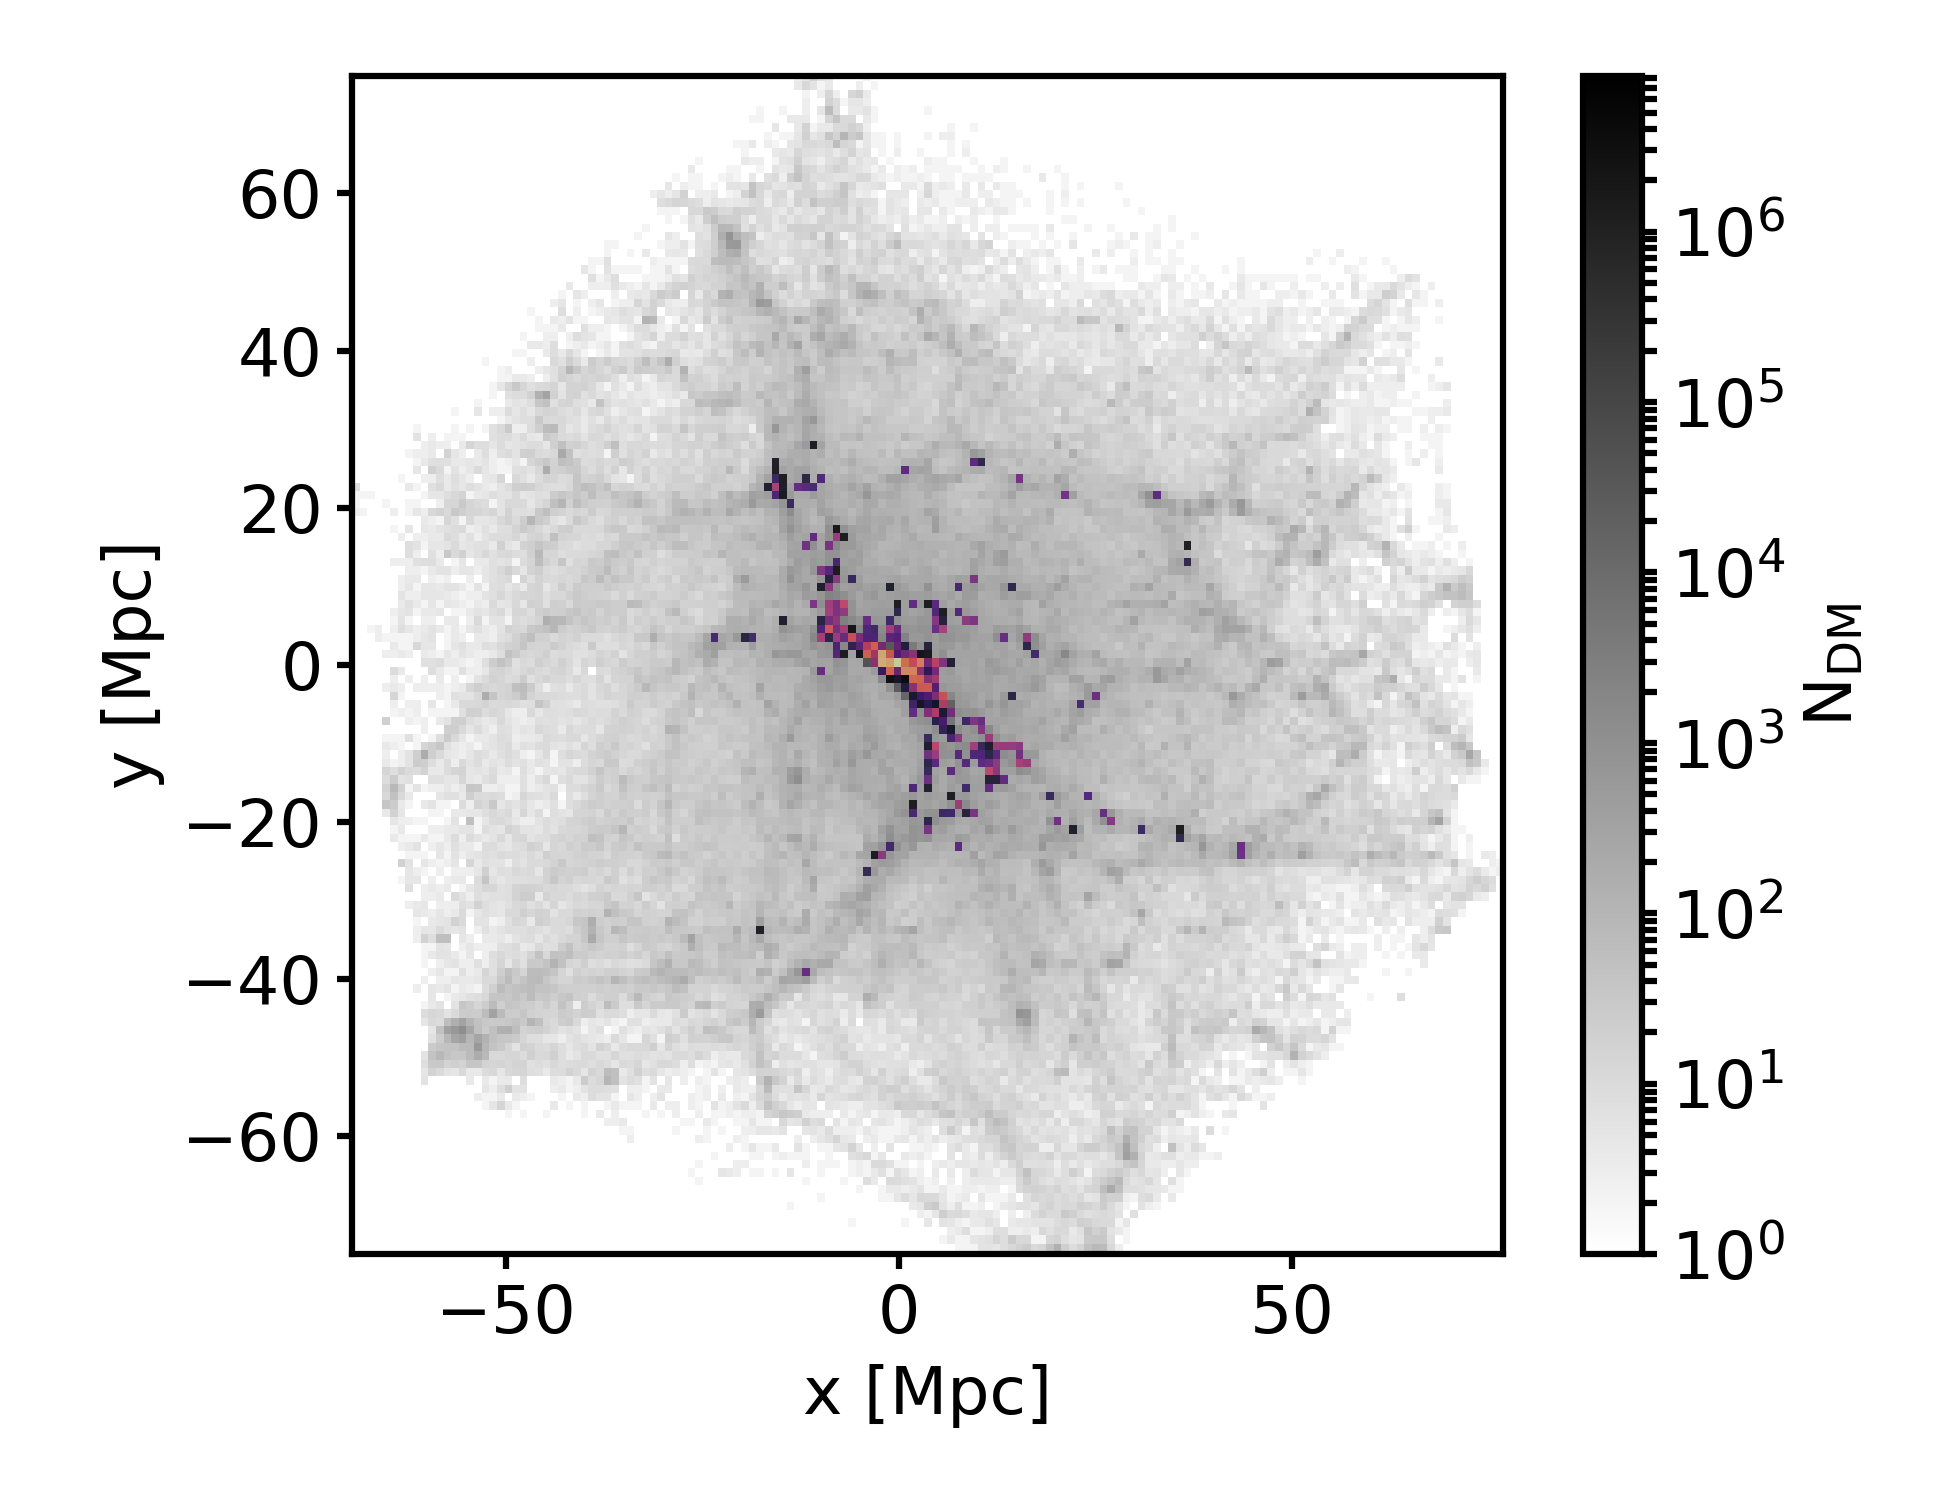
\includegraphics[width=\textwidth]{plots/Auriga/DM_and_stars_xy_distribution.png}
	    \label{fig:DM_stars_xy}
    \end{subfigure}
    
    \begin{subfigure}[b]{0.8\textwidth}
    \centering
    	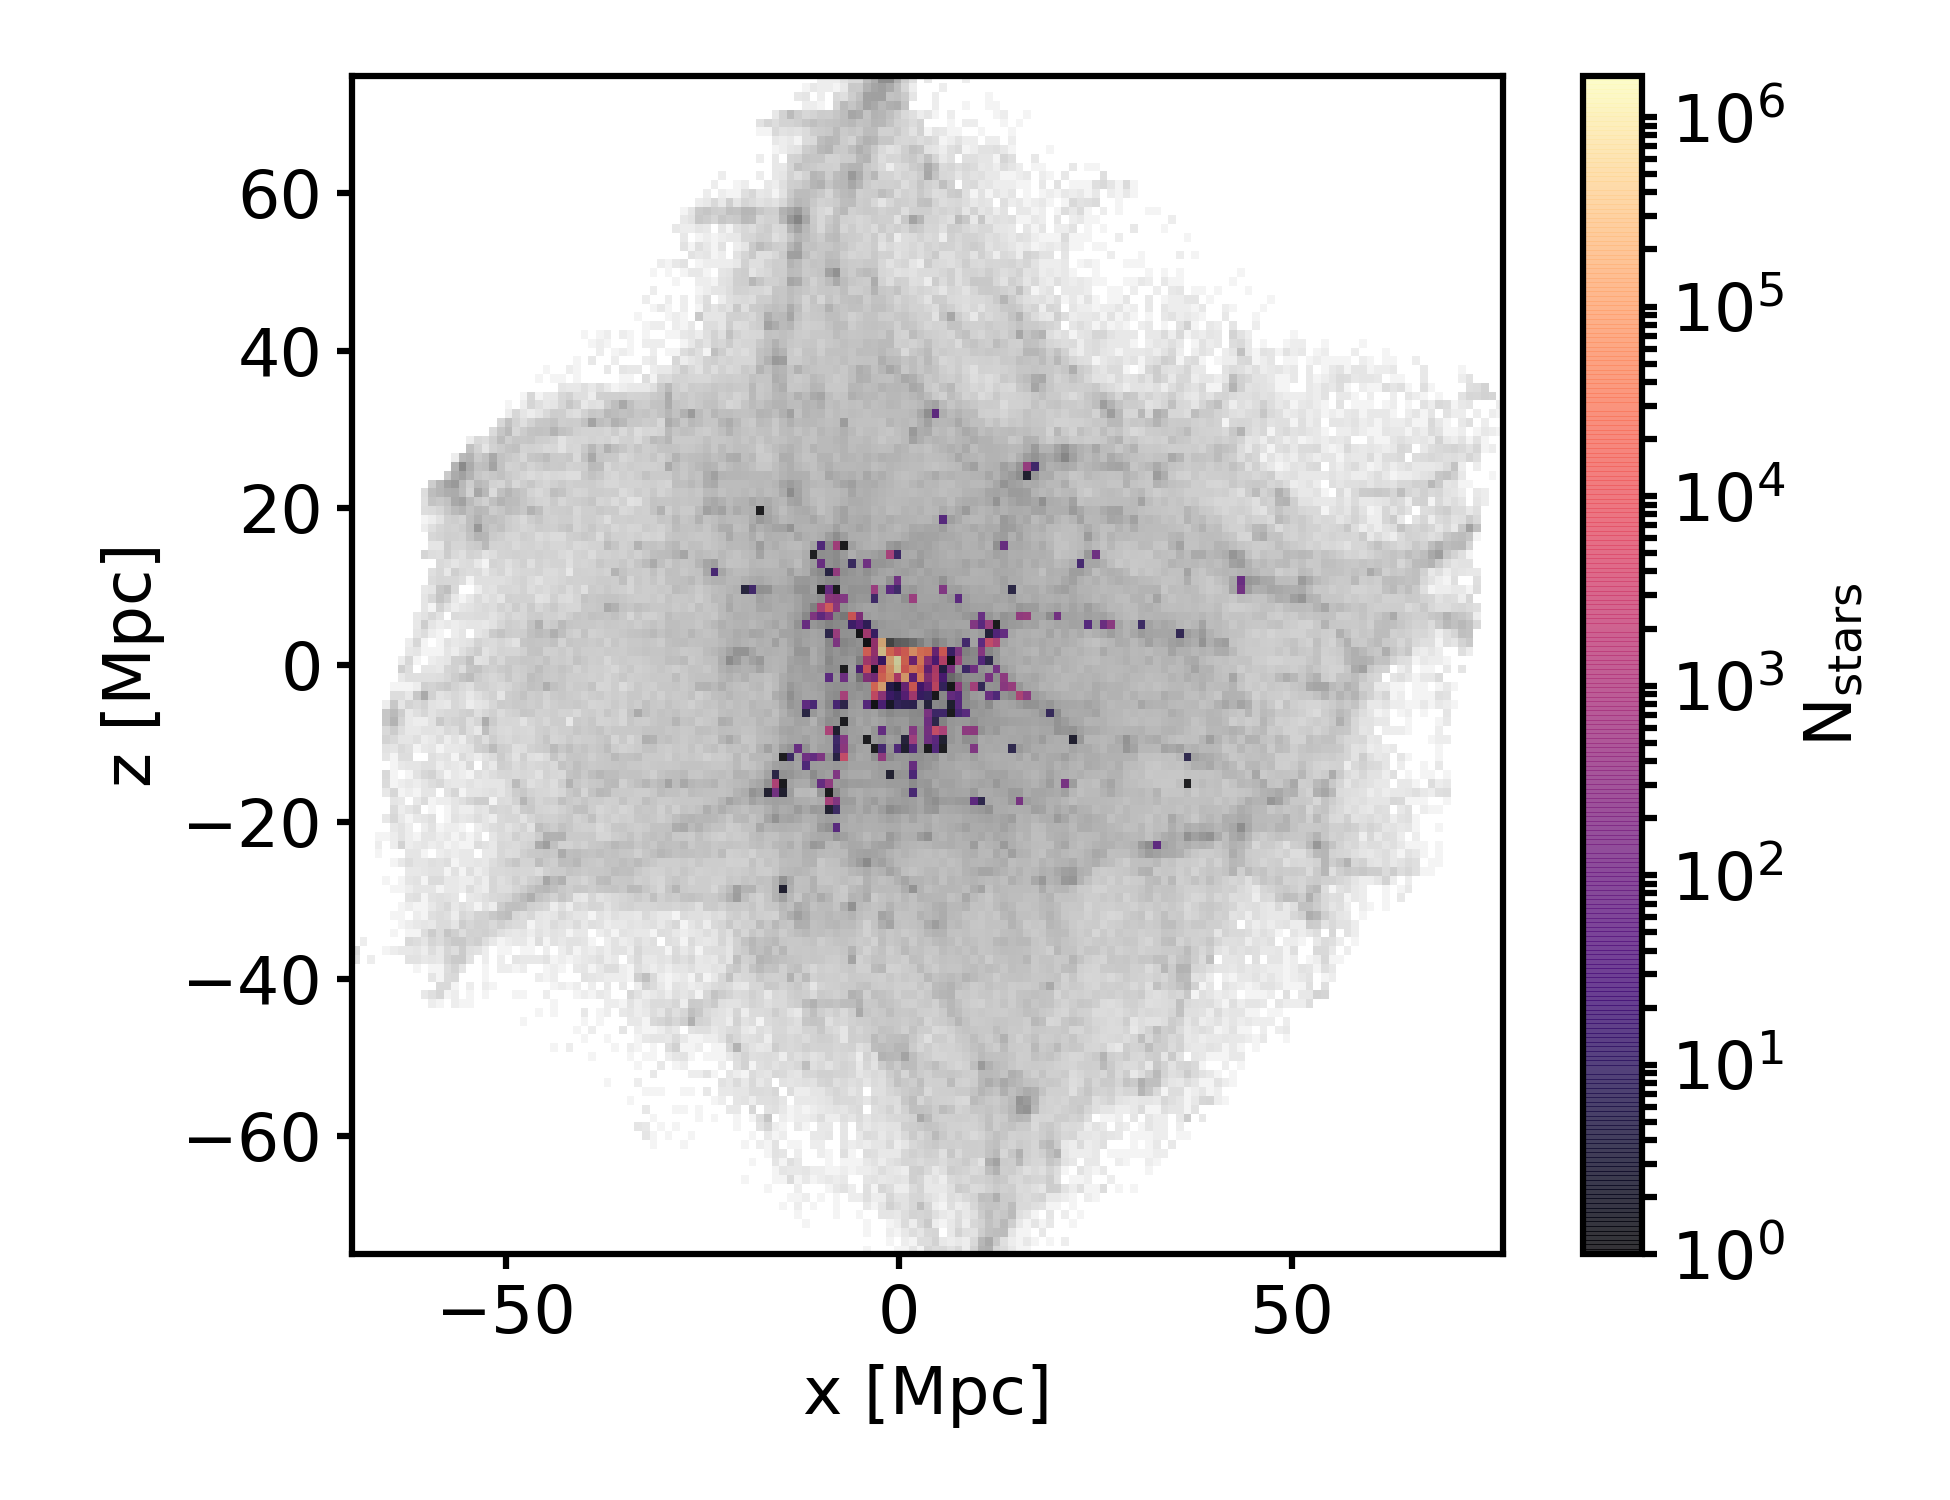
\includegraphics[width=\textwidth]{plots/Auriga/DM_and_stars_xz_distribution.png}
    	\label{fig:DM_stars_xy}
    \end{subfigure}
    \caption{\ac{DM} (grey) and stellar (colors) particle distribution of the whole simulation Auriga24 at $\textit{z}=0$. The \ac{DM} forms the cosmic web, where the mass gathers along its filaments. Baryonic matter also follows these structures. At the most massive parts of the \ac{DM} distribution, the most stellar particles fell in. This structure is typical of hydrodynamical galaxy simulations.}\label{fig:DM_stars_AU24}
\end{figure}
In Figure \ref{fig:DM_stars_AU24}, we show the distribution of \ac{DM} in grey and stars in colors of one selected simulated galaxy (halo 24). The most bound particle is chosen to be the center at $(x,y,z) = (0,0,0)$. The filaments of the \ac{DM} distribution are clearly visible. The stellar particles settle along these filaments and clump inside the densest \ac{DM} structures. 

\subsubsection{Auriga}\label{subsubsec:auriga_intro}
Auriga is a magnetohydrodynamical zoom-in simulation of an isolated \ac{MW} like galaxy. It is build with the moving-mesh AREPO \citep{AREPO} code and includes galaxy physics, active galactic nuclei feedback and magnetic fields. Its goal is to match the observables of the \ac{MW} today and to produce its history which can be compared to observations of spiral galaxies in earlier stages of development. All 30 galaxies are run in normal resolution (\ac{DM} particle mass: $m_\mathrm{DM} = 3\cdot10^5$; Baryonic matter particle mass: $m_\mathrm{b} = 5\cdot10^4$) and 3 selected are run in low ($m_\mathrm{DM} = 2\cdot10^6$; $m_\mathrm{b} = 4\cdot10^5$) and high resolution ($m_\mathrm{DM} = 4\cdot10^4$; $m_\mathrm{b} = 6\cdot10^3$) as well \citep{AurigaGrand}. They are consistent over these three resolution levels and therefore do not rely on numerical parameters but only on physical. Auriga is one of the first simulations where this is accomplished. The snapshots go from redshift $127$, which is close to the beginning of the universe, to redshift $0$, today.  At redshift $z= 0$, different galaxy shapes have evolved. Most of them are spirals but a few are in a merger process. All galaxies have a rich merger history. \citet{AurigaGrand} finds that many properties of the \ac{MW} and \ac{MW} like external galaxies are reproduced by these simulations, such as the mass distribution and the circularity distribution. Others are found to be matching within certain limits, such as the star formation rate–stellar mass relation matches for low redshift $z<1$ but still results in consistent present-day metallicities, mean stellar ages and colours. The set-up and the results of this set of simulations make Auriga one of the most advanced and comprehensive magneto-hydrodynamical galaxy simulations and a very fruitful sample to carry out our investigations. \\
\begin{figure}[htbp]
\captionsetup{format=plain}
    \centering
    \begin{subfigure}[b]{0.8\textwidth}
	    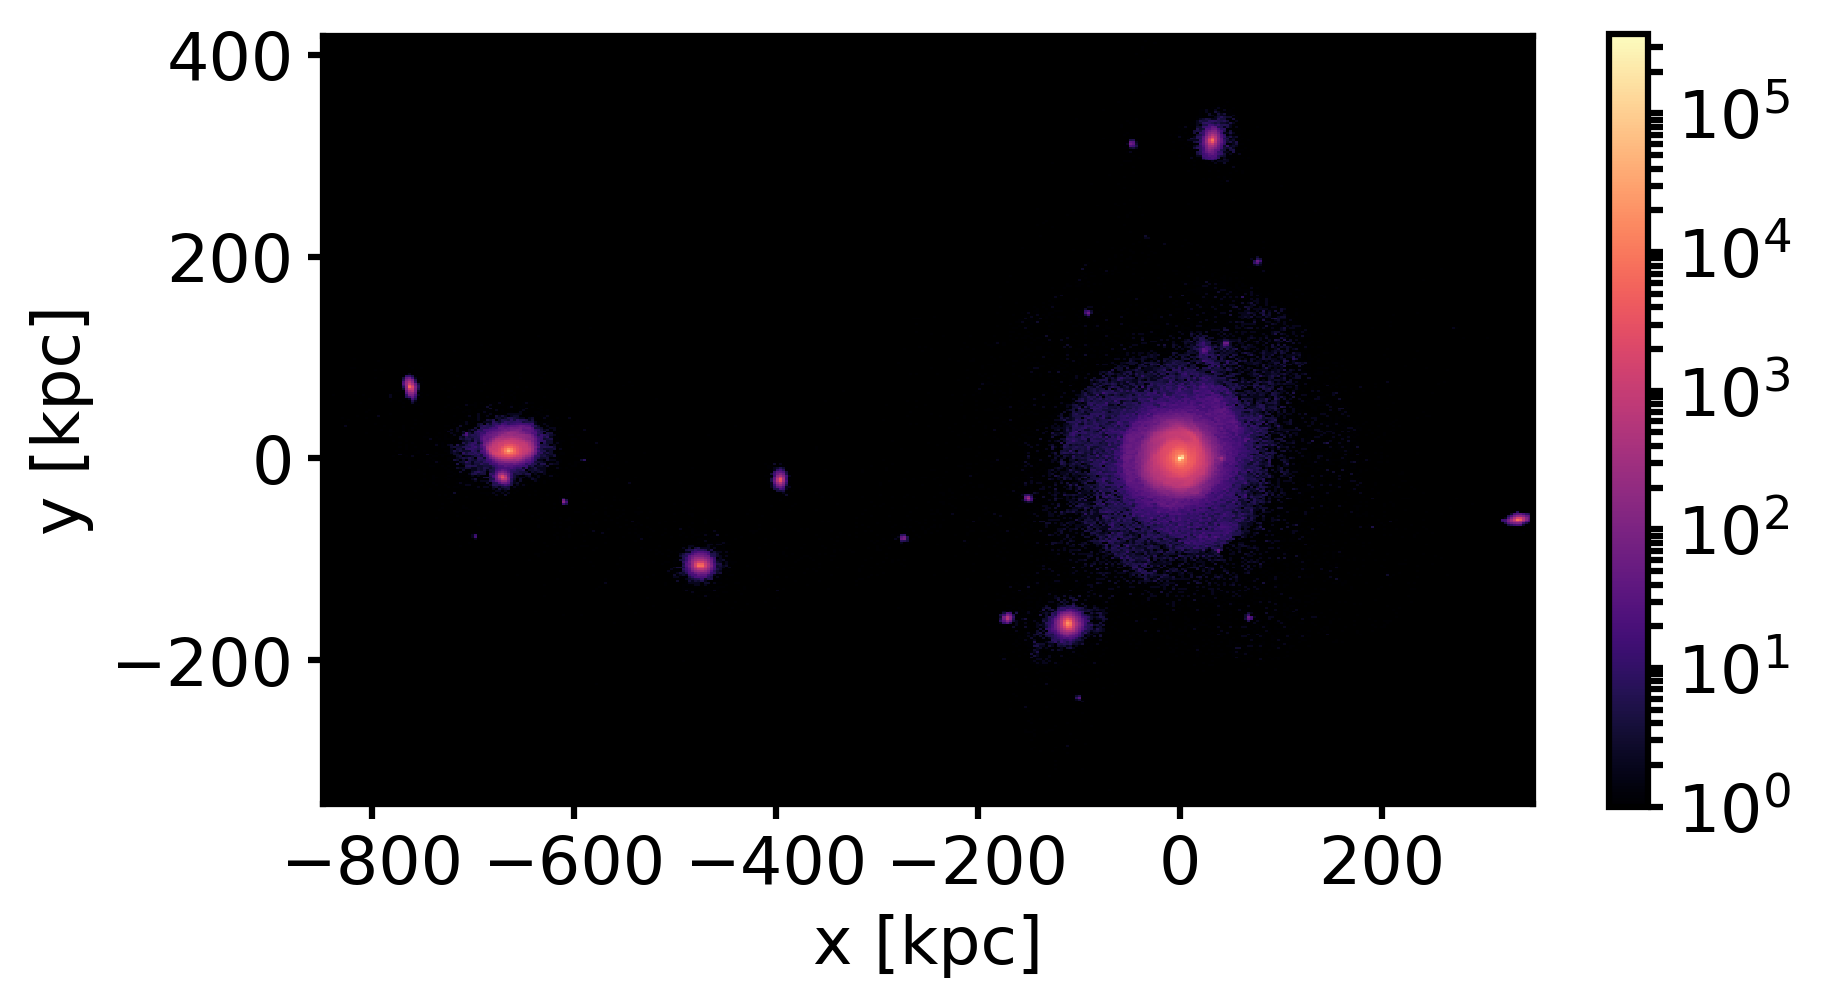
\includegraphics[width=\textwidth]{plots/Auriga/Au24_stars_xy_distribution_halo0.png}
	    \label{fig:Au24_stars_xy}
    \end{subfigure}
    
    \begin{subfigure}[b]{0.8\textwidth}
    \centering
    	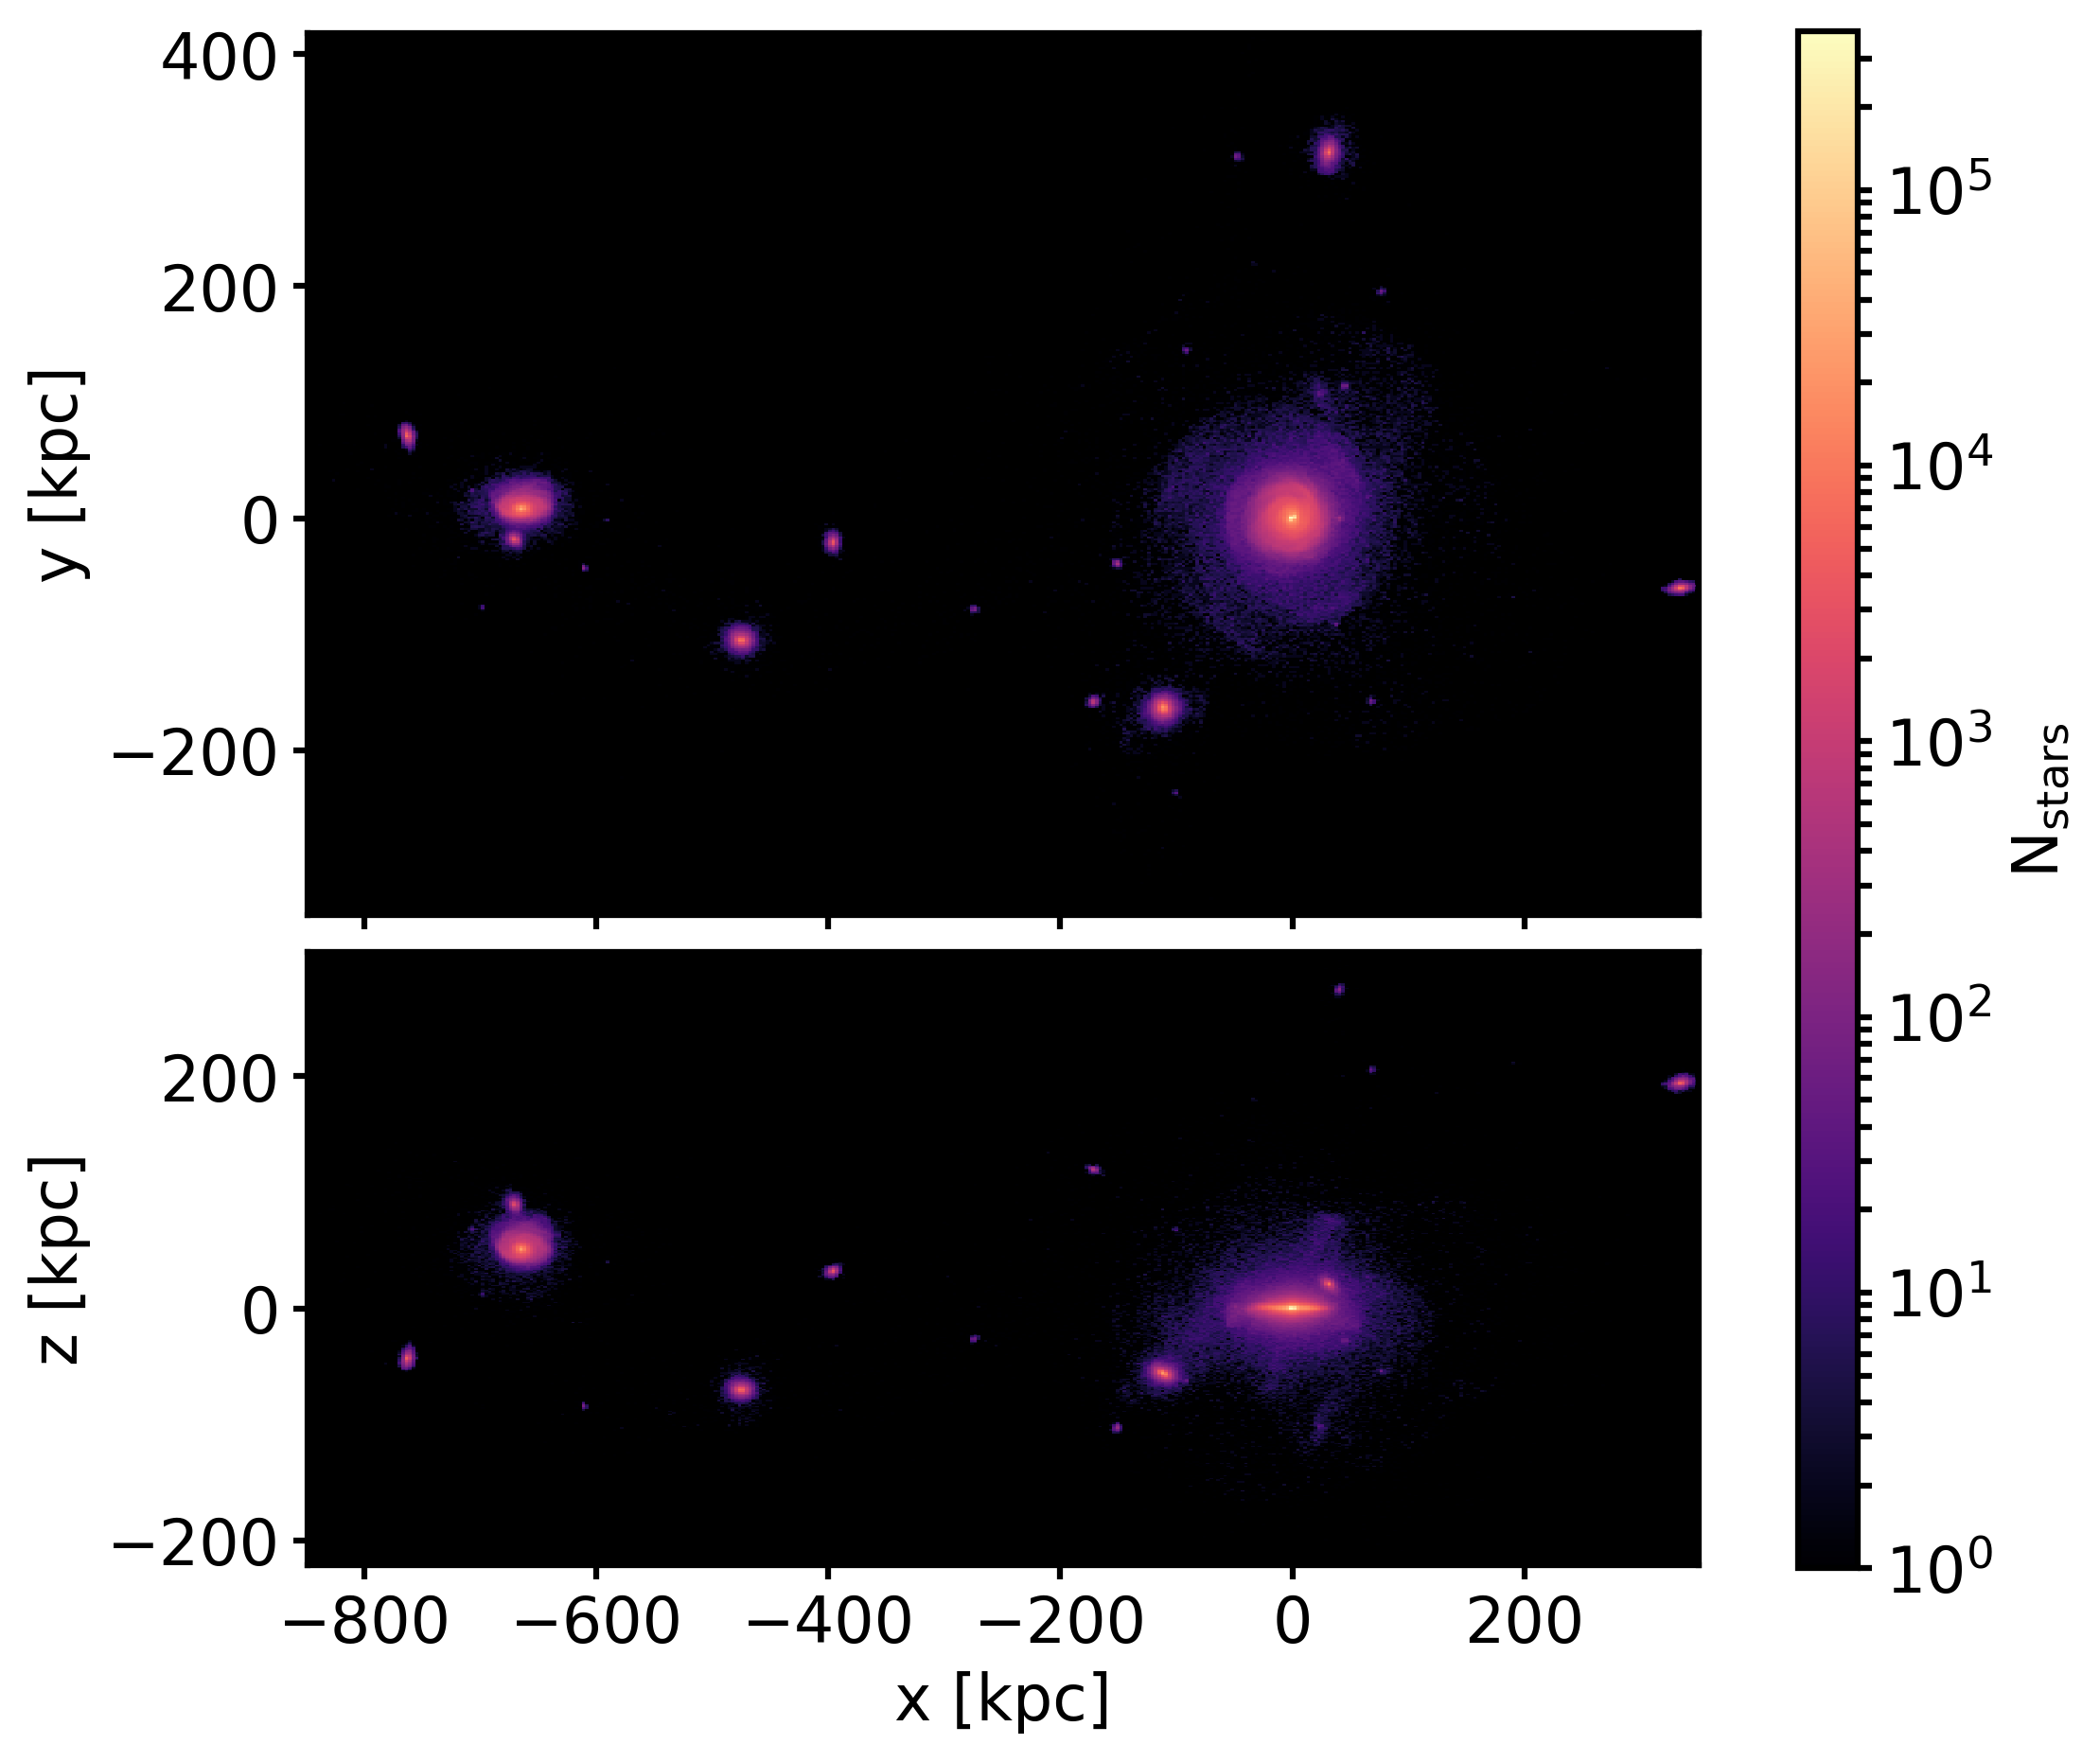
\includegraphics[width=\textwidth]{plots/Auriga/Au24_stars_xz_distribution_halo0.png}
    	\label{fig:Au24_stars_xz}
    \end{subfigure}
    \caption{Stellar distribution of 0th halo at $\textit{z}=0$. The main galaxy is centered at $(0,0,0)$. There are many \acp{DG} around the main galaxy which will eventually merge with it. In the evolution of the simulations, this galaxy has build up mass by merging with \acp{DG}. This mass build up is assumed for and observed in real galaxies.}\label{fig:Stars_AU24}
\end{figure}
\\In Figure \ref{fig:Stars_AU24}, we present the distribution of stellar particles in $x-y$ and $x-z$ direction of the main galaxy in halo 24 and its associated \acp{DG} at redshift $z=0$. Over the course of time, many \acp{DG} already merged with the main galaxy. These make up some of the galaxy's mass and the \ac{DG} stars involved in these mergers are investigated in Section \ref{sec:Dynamics}.\\
\begin{figure}[htbp]
\captionsetup{format=plain}
    \centering
    \begin{subfigure}[b]{0.8\textwidth}
	    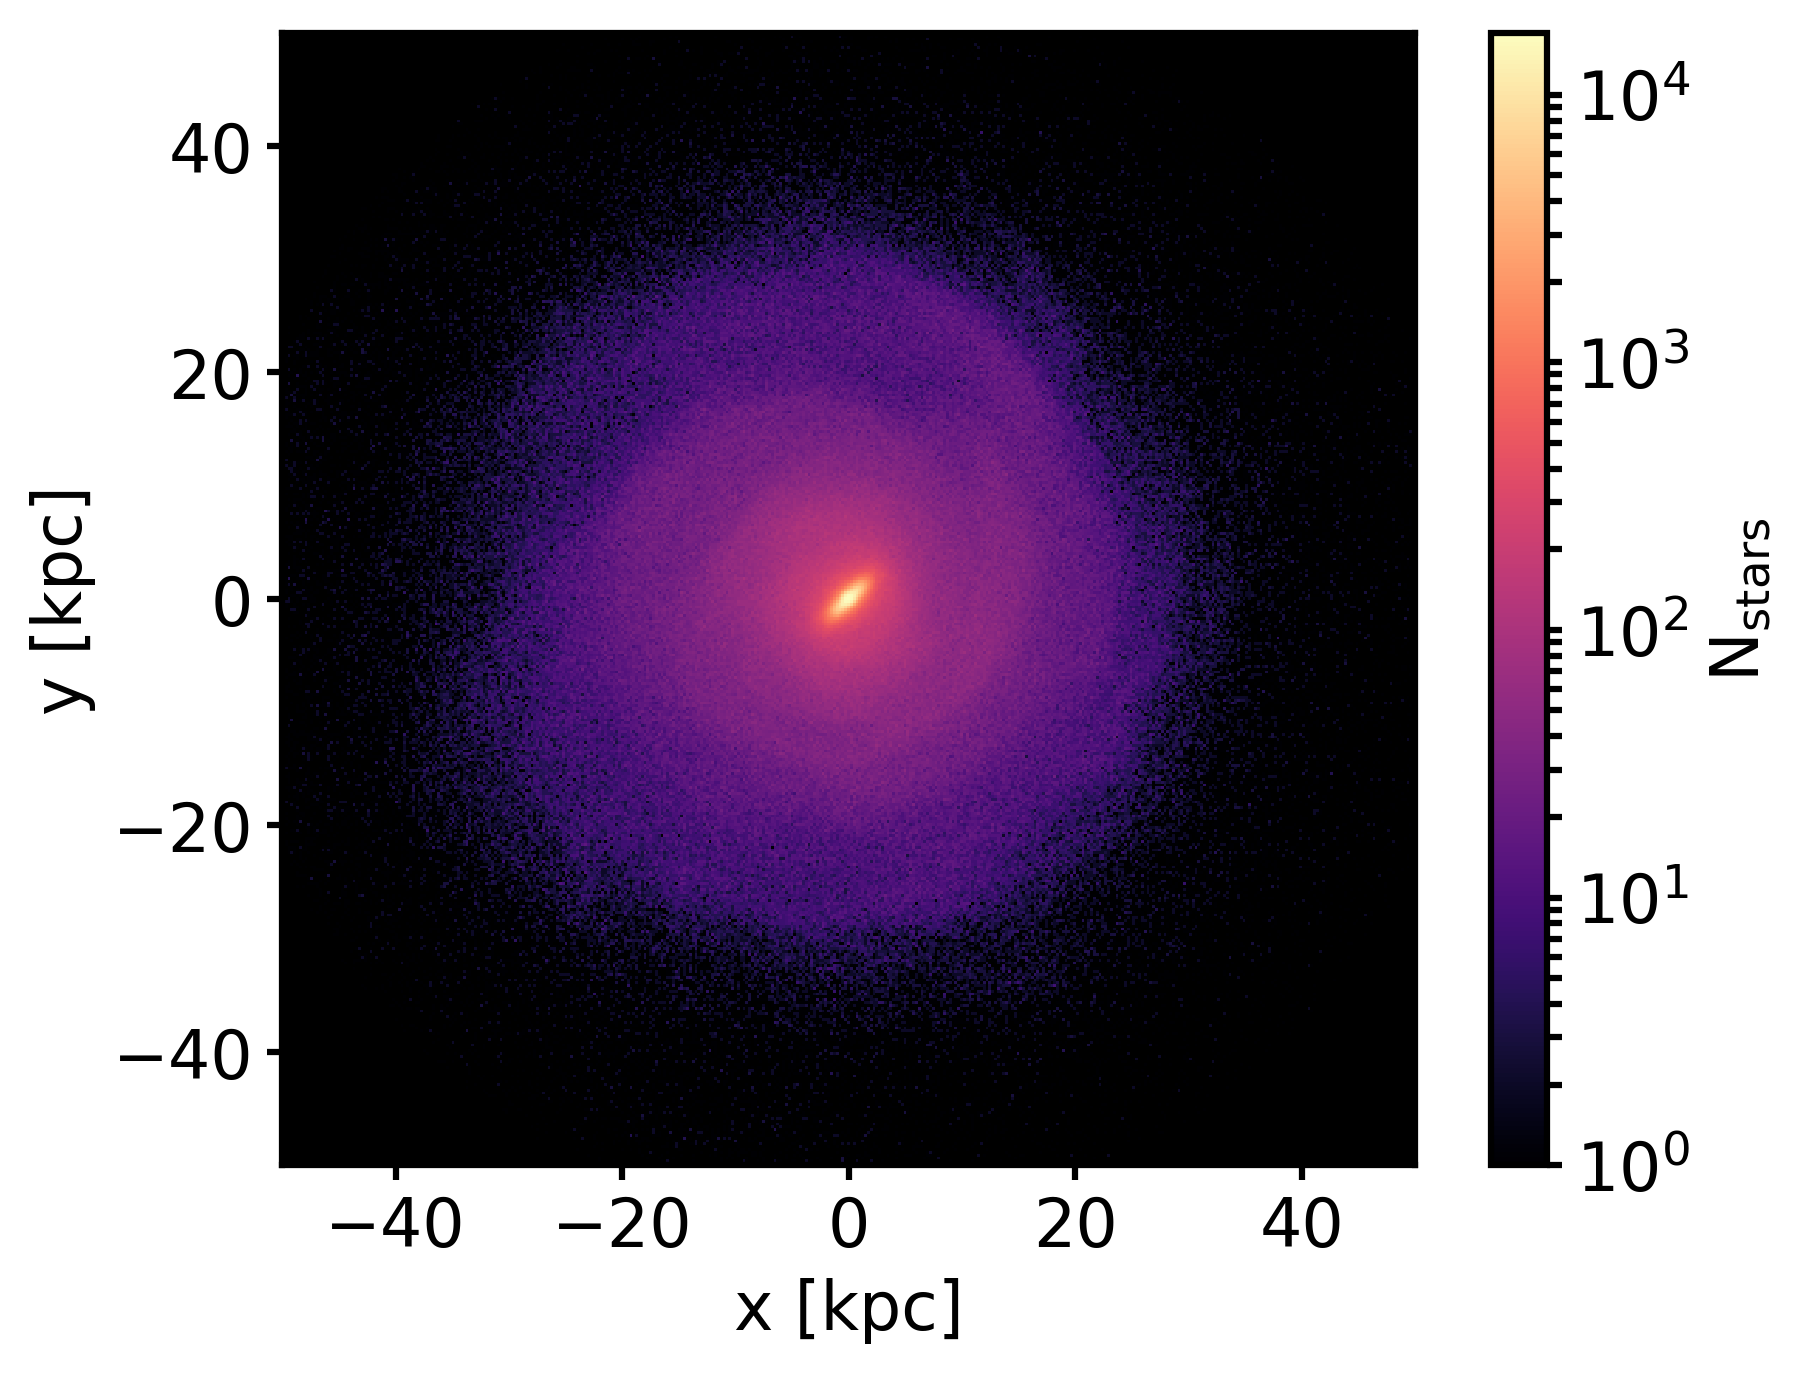
\includegraphics[width=\textwidth]{plots/Auriga/Au24_stars_xy_distribution_halo0_zoomin.png}
	    \label{fig:Au24_stars_xy_zoomin}
    \end{subfigure}
    
    \begin{subfigure}[b]{0.8\textwidth}
    \centering
    	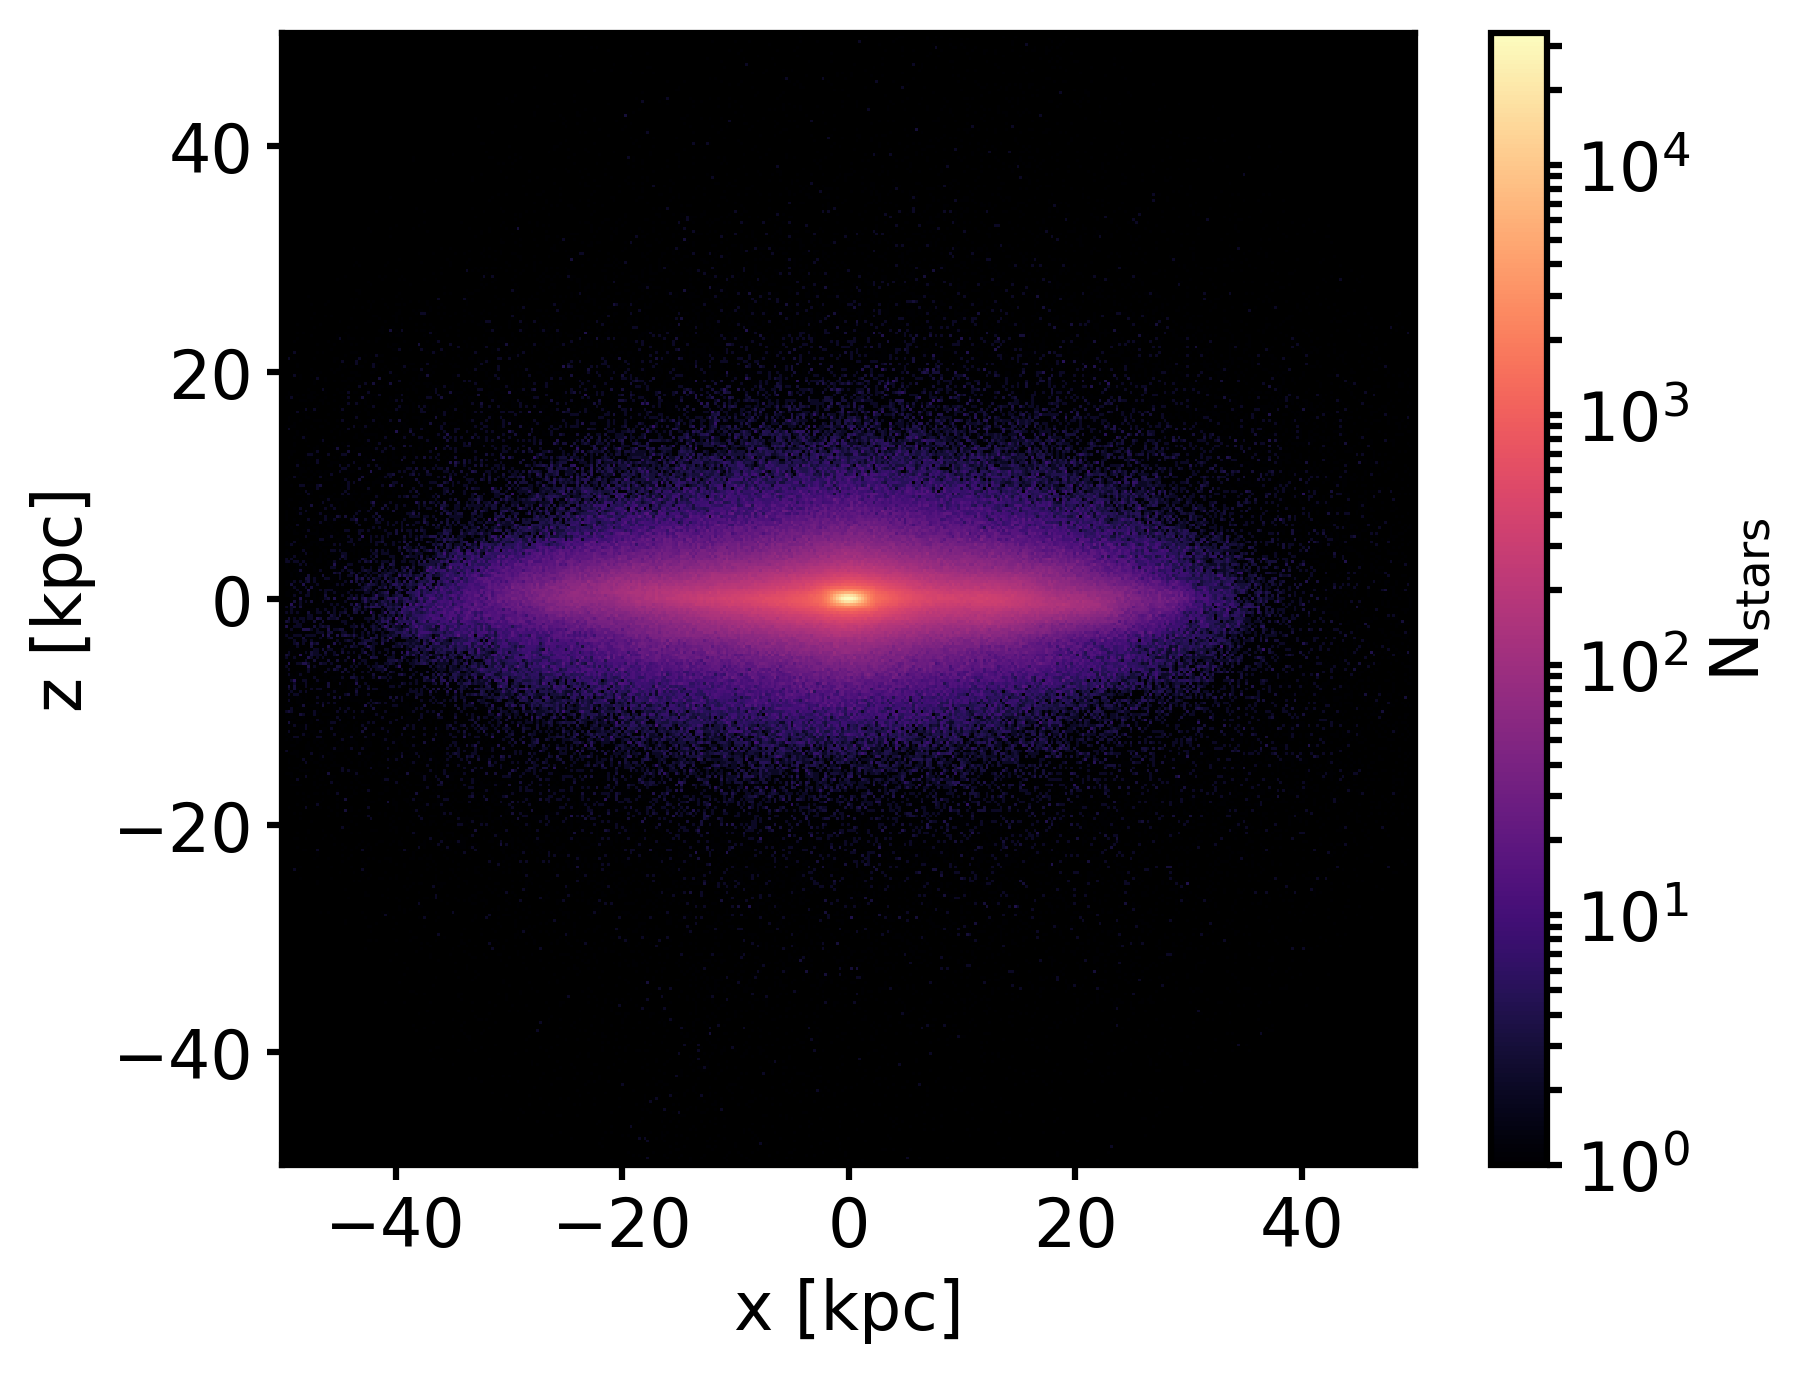
\includegraphics[width=\textwidth]{plots/Auriga/Au24_stars_xz_distribution_halo0_zoomin.png}
    	\label{fig:Au24_stars_xz_zoomin}
    \end{subfigure}
    \caption{Stellar distribution of main galaxy at $\textit{z}=0$. In the upper panel, the galaxy is seen face-on. There, the presence of non-axisymmetric substructure such as spiral arms and a bar is visible. In the lower panel it seen is edge-on. Disk and bulge are clearly present and a close \ac{DG} is visible.}\label{fig:Stars_AU24_zoomin}
\end{figure}
\\A face-on and edge-on view of the main galaxy is presented in Figure \ref{fig:Stars_AU24_zoomin}. We can see axisymmetric features such as bulge and disk and clear non-axisymmetric features such as a bar and spiral arms. This galaxy resembles the \ac{MW} and other late-type galaxies.
\subsection{Fitting axisymmetric potential models}\label{subsec:best_fit_pot}
We require the best fit potential model of this galaxy to be an analytic, axisymmetric, multi-component potential so that we consider this simulations as observers treat external galaxies, since they mostly fit external galaxies with these models (e.g. \citealp{Geehan...Andromedapot...2006}. We need to point out that the galaxy evolved not isolated but went through many mergers and therefore its potential is neither analytic nor axisymmetric but has a lot of substructure. The fit is only an approximation. Also the simulation is self-consistent so changes in potential influence the velocities of the objects inside and changes on the positions of the objects will change the gravitational potential. Since we fit a potential to each snapshot we have a time-dependent potential. The routine and results in this Section are for the $z=0$ snapshot but the same routine was applied for all snapshots since a lookback time of \SI{10.5}{Gyr}. We also need to include a disk and bulge decomposition which is not natural in a cosmological simulation. As the gas evolves in cells, we cannot calculate its density easily. Therefore, we do not consider it in our potential fits. Since we want to recreate observers way of looking at galaxies we do not need to include gas as observers in e.g. Multi-Gaussian Expansion fits \citep{MGE...Monnet, MGE...Emsellem}, that are used in Jeans modelling \citep{Cappellari...Jeans....2008, Glenn....einsteincross...2010}, also only take stellar light into account. 

\subsubsection{About the gravitational potential}\label{subsubsec:pot_theory}
The distribution of stars can be described by their \ac{DF}, $f(\mathbf{x}, \mathbf{v})$ which describes the observed positions and velocities of the stars. They can act as tracers of the gravitational potential $\Phi(\mathbf{x})$. Stars in the disk and the stellar halo are to an extremely good approximation a "collisionless fluid". For these stars, the \ac{CBE} describes their motions: 
\begin{align}\label{eq:CBE}
    \frac{\mathrm{d}f}{\mathrm{d}t} &= \frac{\partial f}{\partial t} + \frac{\partial f}{\partial \mathbf{x}} \cdot \frac{\mathrm{d}\mathbf{x}}{\mathrm{d}t} + \frac{\partial f}{\partial \mathbf{v}} \cdot \frac{\mathrm{d}\mathbf{v}}{\mathrm{d}t}\\
    &= \frac{\partial f}{\partial t} + \bm{\nabla}_x f \cdot \mathbf{v} + \bm{\nabla}_v f \cdot \mathbf{a} = 0.
\end{align}
Applying Newton's gravitational law $\mathbf{F} = -m\bm{\nabla}\Phi(\mathbf{x}) = m\mathbf{a}$ to the last part of the equation and taking the Poisson equation into account to connect $\Phi(\mathbf{x})$ with the total mass we get the important equations:

\begin{empheq}[box=\fbox]{alignat=2}
  &\mathrm{CBE:} \quad&\frac{\mathrm{d}f}{\mathrm{d}t} = \frac{\partial f}{\partial t} + \bm{\nabla}_x f \cdot \mathbf{v} - \bm{\nabla}_v f \cdot \bm{\nabla}_x \Phi(\mathbf{x}) \label{eq:CMB_phi}\\
  &\mathrm{Poisson:}\quad&\bm{\nabla} \cdot \bm{\nabla} \Phi(\mathbf{x})= \bm{\nabla}^2 \Phi(\mathbf{x}) =4\pi G \rho(\mathbf{x}) \label{eq:Poisson}
\end{empheq}
with the gravitational constant $G$ and the total mass density of stars, gas and \ac{DM}, $\rho(\mathbf{x})$. 
If the system is in "steady state", $\partial f/\partial t = 0$, distribution functions that are functions of the \ac{IoM} solve Equation \ref{eq:CMB_phi} (see Section \ref{sec:Dynamics}). The Poisson equation, Equation \ref{eq:Poisson}, is used to link densities and potentials in the upcoming descriptions of the potentials of the single components and presents a direct link between the gravitational potential and the total mass. 

\subsubsection{galpy - A python package for galactic dynamics}\label{subsubsec:galpy}
galpy \citep{Bovy...galpy...2015} is a well tested and well documented python package for galactic dynamics that is being developed on \url{http://github.com/jobovy/galpy}. The latest documentation can be found at \url{http://galpy.readthedocs.org/en/latest/}. It includes analytic spherical, axisymmetric and ellipsoidal triaxial potentials and fast routines, additionally implemented in C, for the calculation of orbits, action-angles and \acp{DF}. galpy has its own internal units which have to be considered and understood before using it.
\\In this work, we first fit a set of analytic potentials to the simulation which is described in the remainder of this Section. Then, we calculate actions of accreted \acp{GC} in a variety of potentials in galpy and investigate the results in the next Section. 

\subsubsection{Component decomposition}\label{subsubsec:decomp}
To fit a potential to each component, we first need to decompose the different parts. We assume that all \ac{DM} particles belonging to the main galaxy make up its halo. The stellar particles belong to either the central spheroid or the disk. We distinguish these components by the use of the circularity parameter \citep{Abadi...circularity...2003}
\begin{equation}\label{eq:circularity}
    \epsilon = \frac{L_z}{L_{z,max}(E)}
\end{equation}
where $L_{z,max}(E)$ is the maximum angular momentum allowed for the orbital energy $E$. 
$\epsilon = 1$ is a prograde circular orbit in the disc plane. $\epsilon = -1$ is a retrograde circular orbit in the disc plane. $\epsilon \sim 0$ is an orbit with a very low $z$-component of angular momentum which may be highly inclined to the disc spin axis and/or be highly eccentric.  

\cite{AurigaGrand} uses two different methods two distinguish the components and to get their mass ratio:
\begin{enumerate}
\item Under the assumption, that the bulge has zero net rotation, mirror negative $\epsilon$ as bulge material, the rest belongs to the disk.
\item All particles with $\epsilon > \mathrm{constant}$ are assigned to the disk, where $\mathrm{constant} = 0.7$ is set heuristically.
\end{enumerate}

\cite{AurigaGrand} find that the first method generally overestimates the \ac{D/T} ratio while the second approach underestimates it by choosing only kinematically very cold particles. Since we do not only want to get the mass ratio of \ac{D/T} but also want to tag each particle clearly, we use the second method. Nevertheless, the true assignment lies somewhere between these methods. 
\begin{SCfigure}%[htbp]
\captionsetup{format=plain}
    \centering
    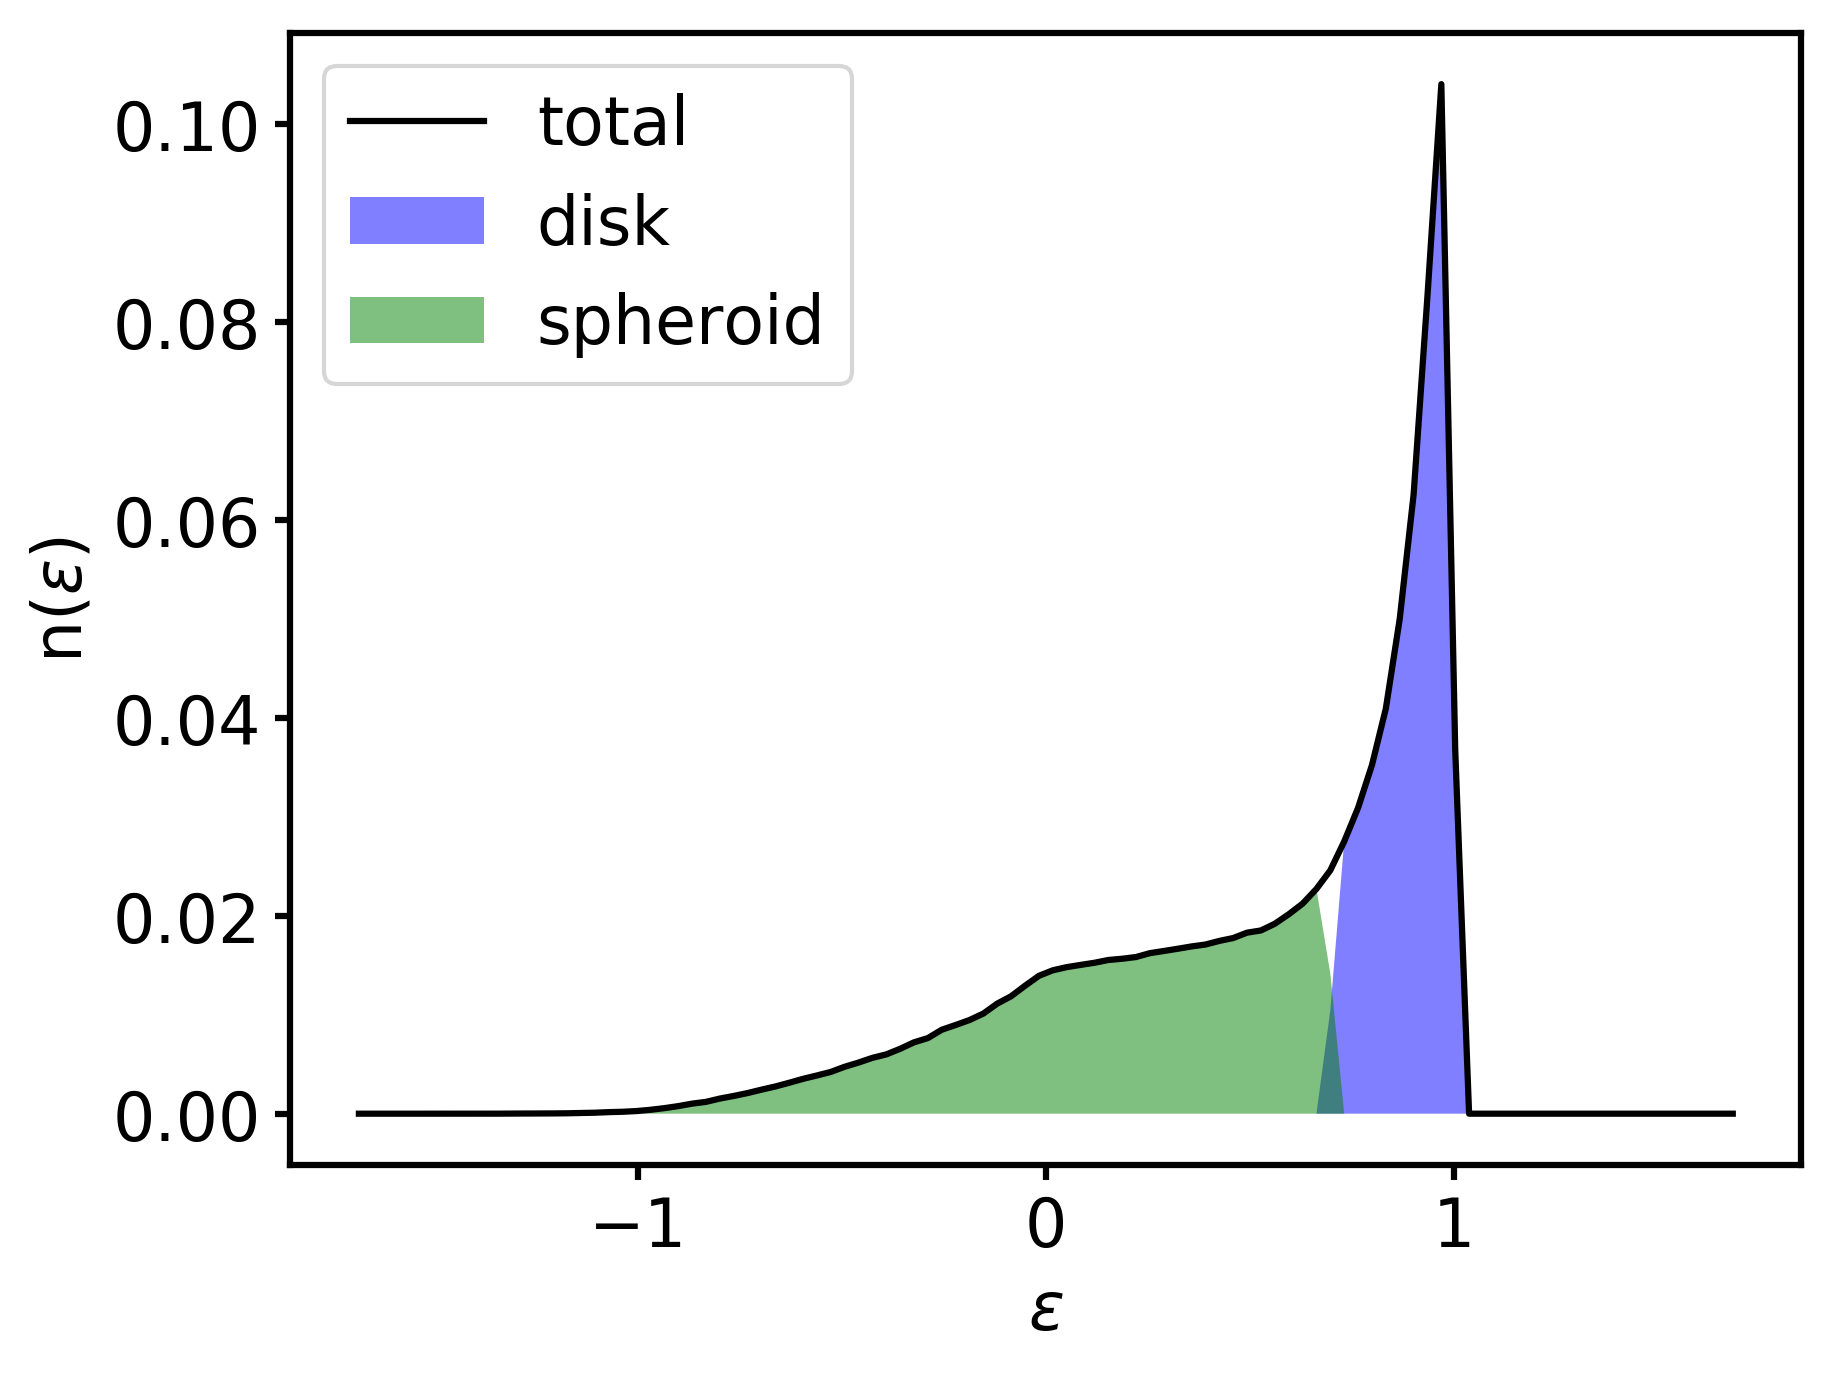
\includegraphics[width=0.6\textwidth]{plots/Auriga/decomposition_snap_127.png}
\caption{Decomposition of stellar disk and spheroid by their circularity. It was carried out for all stellar particles within the galaxy radius. The black line represents the total circularity. The green area is the the spheroid component and the blue is the disk component. The disk particles were selected by having a circularity above 0.7. The disk to total number ratio is 0.47. \textcolor{red}{update ylabel coming}}\label{fig:decomposition}
\end{SCfigure}
\\In Figure \ref{fig:decomposition}, we show a histogram of the circularity with our decomposition. The blue part is the disk portion while the green part is the spheroid. Together they add up to the black solid line, the total number. The \ac{D/T} ratio is 0.47.
Since we can assign the particles to be in the spheroid or disk easily, we use this composition to find the disk and spheroid where we fit our potential to. 


\subsubsection{Disk potential}\label{subsubsec:disk_pot}
We fit the disk with a \citet{MNprofile} (\acsu{MN}) potential following the profile 
\begin{equation}\label{eq:MND}
\Phi(R,z) = -\frac{GM}{\sqrt{R^2+(a+\sqrt{z^2+b^2})^2}}
\end{equation} 
with scale length $a$ and scale height $b$ which provides a disk with a finite thickness. If $b\rightarrow 0$, the disk will be infinite thin and if $a \rightarrow 0$, the potential has a spherical density distribution. $b/a$ therefore defines the flattening of the system. It is a rather simple model with only small computational costs as forces and densities can be calculated analytically from Equation \ref{eq:MND}. Therefore it is widely used. It has limitations in the mid-plane ($z=0$) at high $R$ as the density behaves as $R^−3$ for $R\gg a$ and the large-radius density fall-off is therefore simply a power-law of $R$ rather than exponential. The \ac{MN} density remains too high at large radii (e.g., at $R\gg15$ kpc for the \ac{MW}) compared to realistic models of galactic disks. 
\\To fit the disk potential, we bin the stellar disk in $(R, z)$ and calculate the density of each bin. Then, we fit the \ac{MN} density to the data using the scipy \citep{scipy....2001} routine optimize.curve\_fit. For the \ac{MN} potential, we have the scale length $a_{\mathrm{MND}}$, the scale height $b_{\mathrm{MND}}$ and the contribution to the total circular velocity $v_{0, \mathrm{MND}}$ at $ R_0 = \SI{8}{kpc}$ as fit parameters. The best fit parameters are listed in Table \ref{tab:pot_best_fit_params}.
\begin{figure}[htbp]
\captionsetup{format=plain}
    \centering
    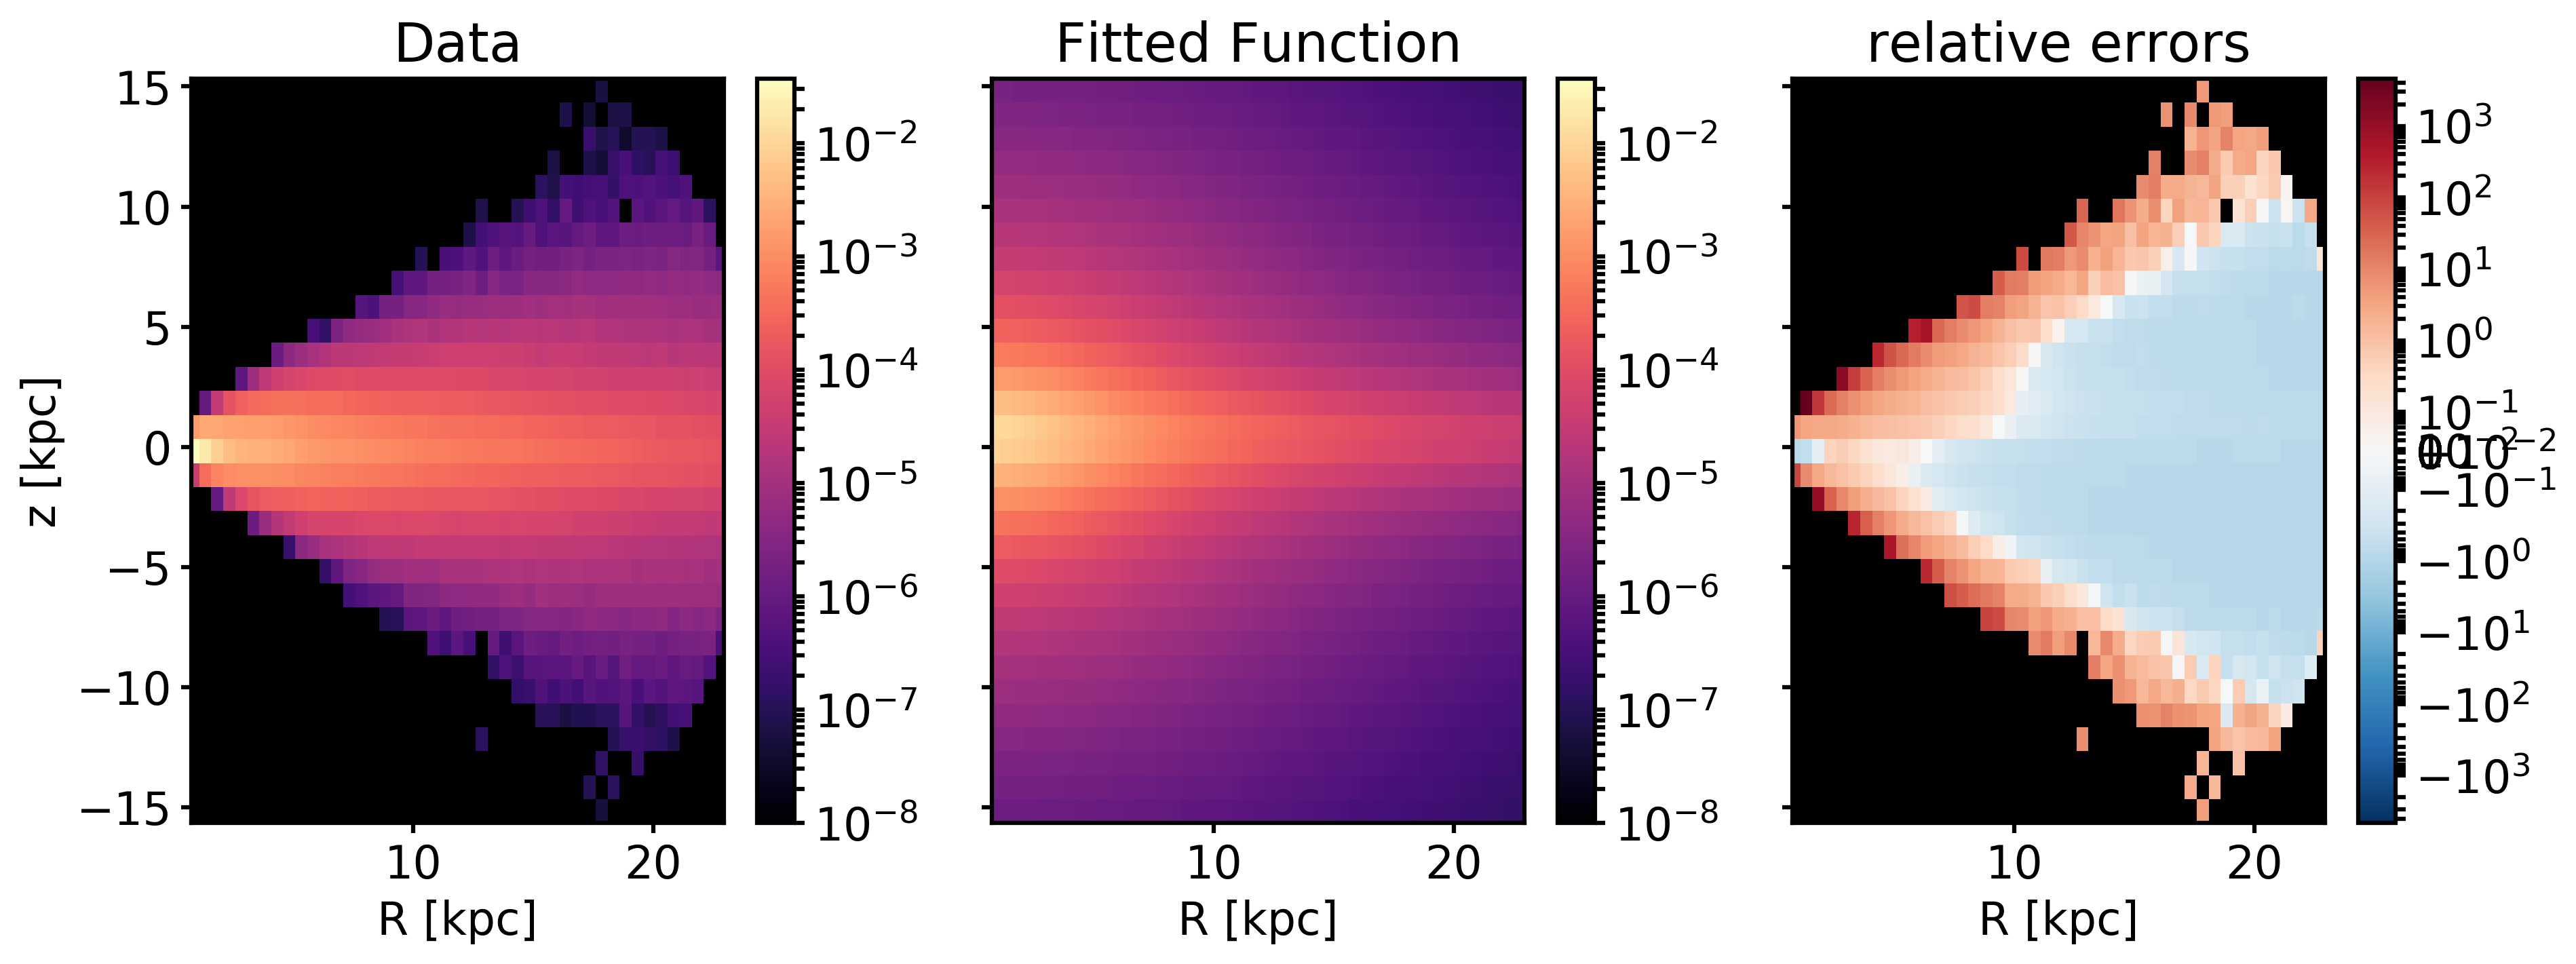
\includegraphics[width = \textwidth]{plots/Auriga/MND_best_fit_snap_127.png}
    \caption{Density fit of the \ac{MN} profile to the disk. \textit{Left panel:} in $(R,z)$ binned mass density of the simulation data. \textit{Middle panel:} in $(R,z)$ binned mass density of the best fit \ac{MN} profile. \textit{Right panel:} relative errors \(\Delta_\rho = (\rho_{\mathrm{fit}}- \rho_{\mathrm{data}})/\rho_{\mathrm{data}}\) of the best fit.}
    \label{fig:MND}
\end{figure}
\\The best fit is shown in Figure \ref{fig:MND}. In the left panel, we see the binned data. Due to the kinematic selection of disk particles, the disk appears to be flaring. This is negligible since the density falls off quickly above an absolute height of \SI{1.5}{kpc}. At the black parts of the histogram, there was no data. Therefore, they weights of the fit lay on the actual disk. In the middle panel, we show the binned density of the best fit \ac{MN} profile. We can clearly see the disk. Since it is an analytic potential, the density can be calculated for every bin in $(R, z)$. In the right panel, the relative errors \(\Delta_\rho = (\rho_{\mathrm{fit}}- \rho_{\mathrm{data}})/\rho_{\mathrm{data}}\) are plotted. In the edges of the data, these errors are very high. This is most probably due to selection effects and cutting the data there while the fitted density is still smooth there. In the disk and outer regions, the relative error is smaller than at the edges. We discuss problems with the disk fit in Section \ref{subsec:wrong_pot_fit}. Even though the errors are quite big, we think this is the best fit of the analytic \ac{MN} potential to the non-analytic and selected-through-decomposition disk. 


\subsubsection{Spheroid potential}\label{subsubsec:spher_pot}
For the central stellar spheroid, we apply a \citet{Hernquistprofile} potential which has the density 
\begin{equation}
    \rho = \frac{M}{2\pi}\frac{a}{r}\frac{1}{(r+a)^3}
\end{equation}
where $M$ is the stellar mass of the spheroid and $a$ is its scale length. It has a gentle power-law cusp and at large radii, it declines like $r^{-4}$. \citet{Hernquistprofile} has shown that it reproduces properties of elliptical galaxies and spherical bulges. 
\\
\begin{SCfigure}
\captionsetup{format=plain}
    \centering
    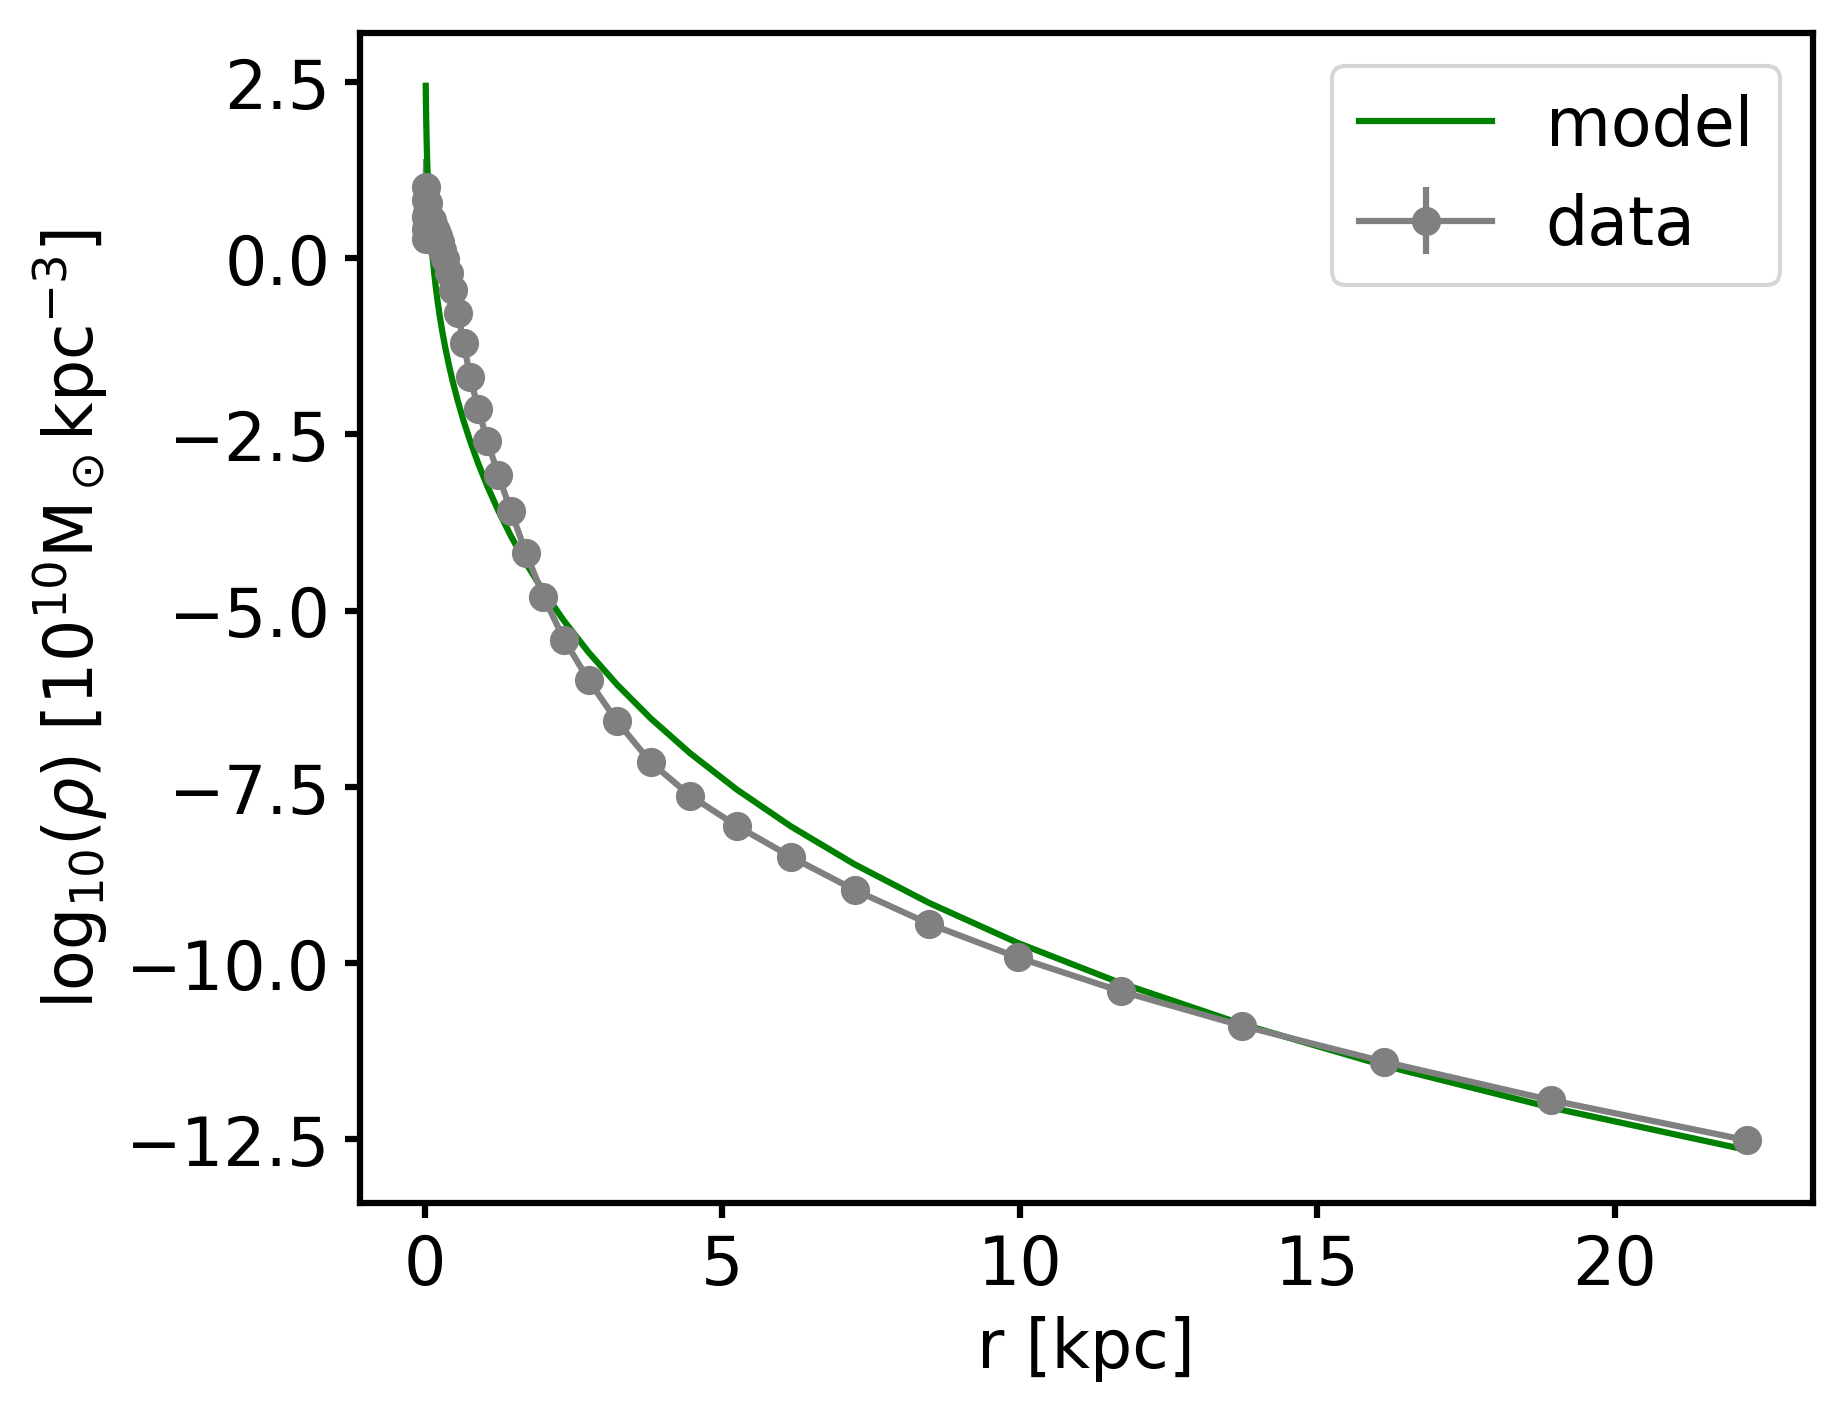
\includegraphics[width=0.7\textwidth]{plots/Auriga/spheroid_density_fit_snap_127.png}
    \caption{Spheroid density: data with errors (grey dots) and best fit (green line). The data is binned logarithmically in r. Their standard deviation is too small to be seen. In the inner part, r $<10$kpc, the density is both under and over estimated. In the outer parts, the fit matches the data. \textcolor{red}{update ylabel coming}}
    \label{fig:spheroid_fit}
\end{SCfigure}
\\Since the Hernquist density is spherically symmetric, we bin the spheroid particles to logarithmic bins in the spherical radius $r$. The data and best fit densities are shown in Figure \ref{fig:spheroid_fit}. While in the inner part the fit does not match the data too well, in the outer parts it fits. Since most of the particles we investigate in Section \ref{sec:Dynamics} are more far away from the center than \SI{10}{kpc}, the fit is acceptable to carry out this analysis.

\subsubsection{Halo potential}\label{subsubsec:halo_pot}
We model the \ac{DM} halo with a \acsu{NFW} \citep{NFWprofile} profile following the formula 
\begin{equation}
    \rho(r) = \frac{\rho_{crit} \cdot \delta_c}{(r/r_s)(1+r/r_s)^2} = \frac{M}{4 \pi a^3}\frac{1}{(r/a)(1+r/a)^2}
\end{equation} with scale radius $r_s = a$, the critical density $\rho_{crit} = 3H^2 / 8\pi G $, the mass $M$ of the \ac{DM} halo and a characteristic and dimensionless density $\delta_c$ which can be rewritten as \(\rho_{crit}\cdot\delta_c = M/4\pi a^3 \). The \ac{NFW} profile is derived from \ac{DM} only hydrodynamical simulations and found to accurately describe \ac{DM} halos. 
\\All particles in the simulation have a potential value, 'pot',  which is the potential they feel at their position from the total surrounding matter (not only from the host galaxy). Since the total halo (shown in Figure \ref{fig:Stars_AU24}) is isolated and the main matter contribution comes from the main galaxy and its halo, we still consider this a value where we can fit the potential of the analytic model to. 
\begin{figure}[htbp]
\captionsetup{format=plain}
    \centering
    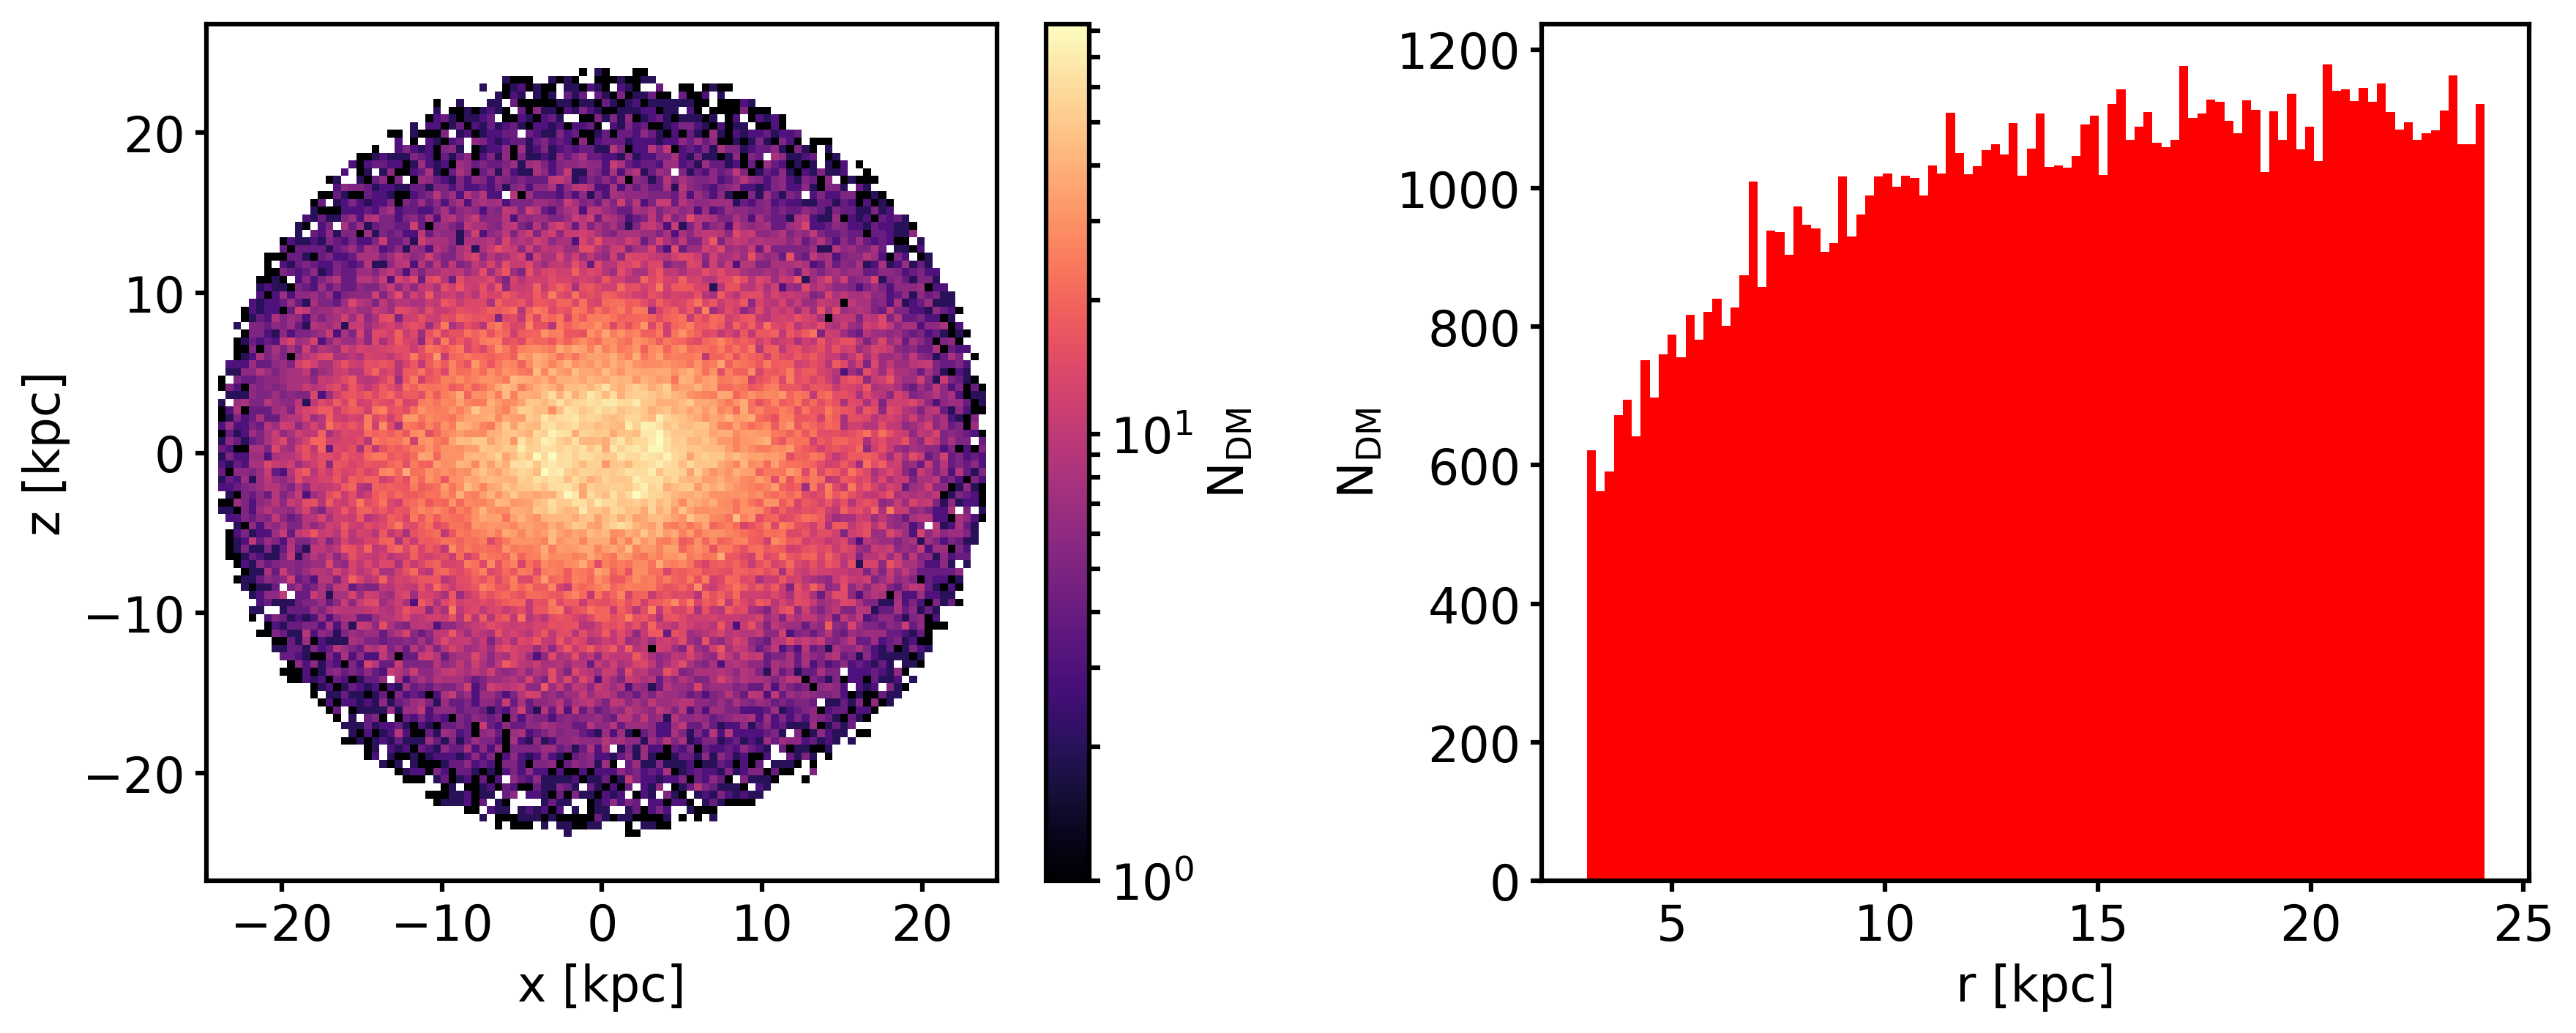
\includegraphics[width=\textwidth]{plots/Auriga/DM_selected_part_dist_snap_127.png}
    \caption{Selection of 100000 random \ac{DM} particles, used to fit to the \ac{NFW} halo. \textit{Left panel:} Distribution of particles in the x-z plane. \textit{Right panel:} Number of \ac{DM} particles depending on r. For radii > \SI{10}{kpc}, the distribution is constant while there are less particles for smaller radii. Since we are less interested in the innermost part of the halo, it is good that the weight for the fit lies in the outer parts. \ac{DM} particles with $r < \SI{3}{kpc}$ are excluded from the fit since it worsened the fit in the outer parts.}
    \label{fig:DM_part_selection}
\end{figure}
We select 100000 \ac{DM} particles randomly which we present in Figure \ref{fig:DM_part_selection}. With the best fit potentials for the stellar components, we set up a potential in galpy with all three components. We calculate the value of the potential for each of the randomly selected particles in the model and fit these to the true potential with the scipy.optimize.differential\_evolution routine by minimizing their squared relative errors.
\begin{SCfigure}
\captionsetup{format=plain}
    \centering
    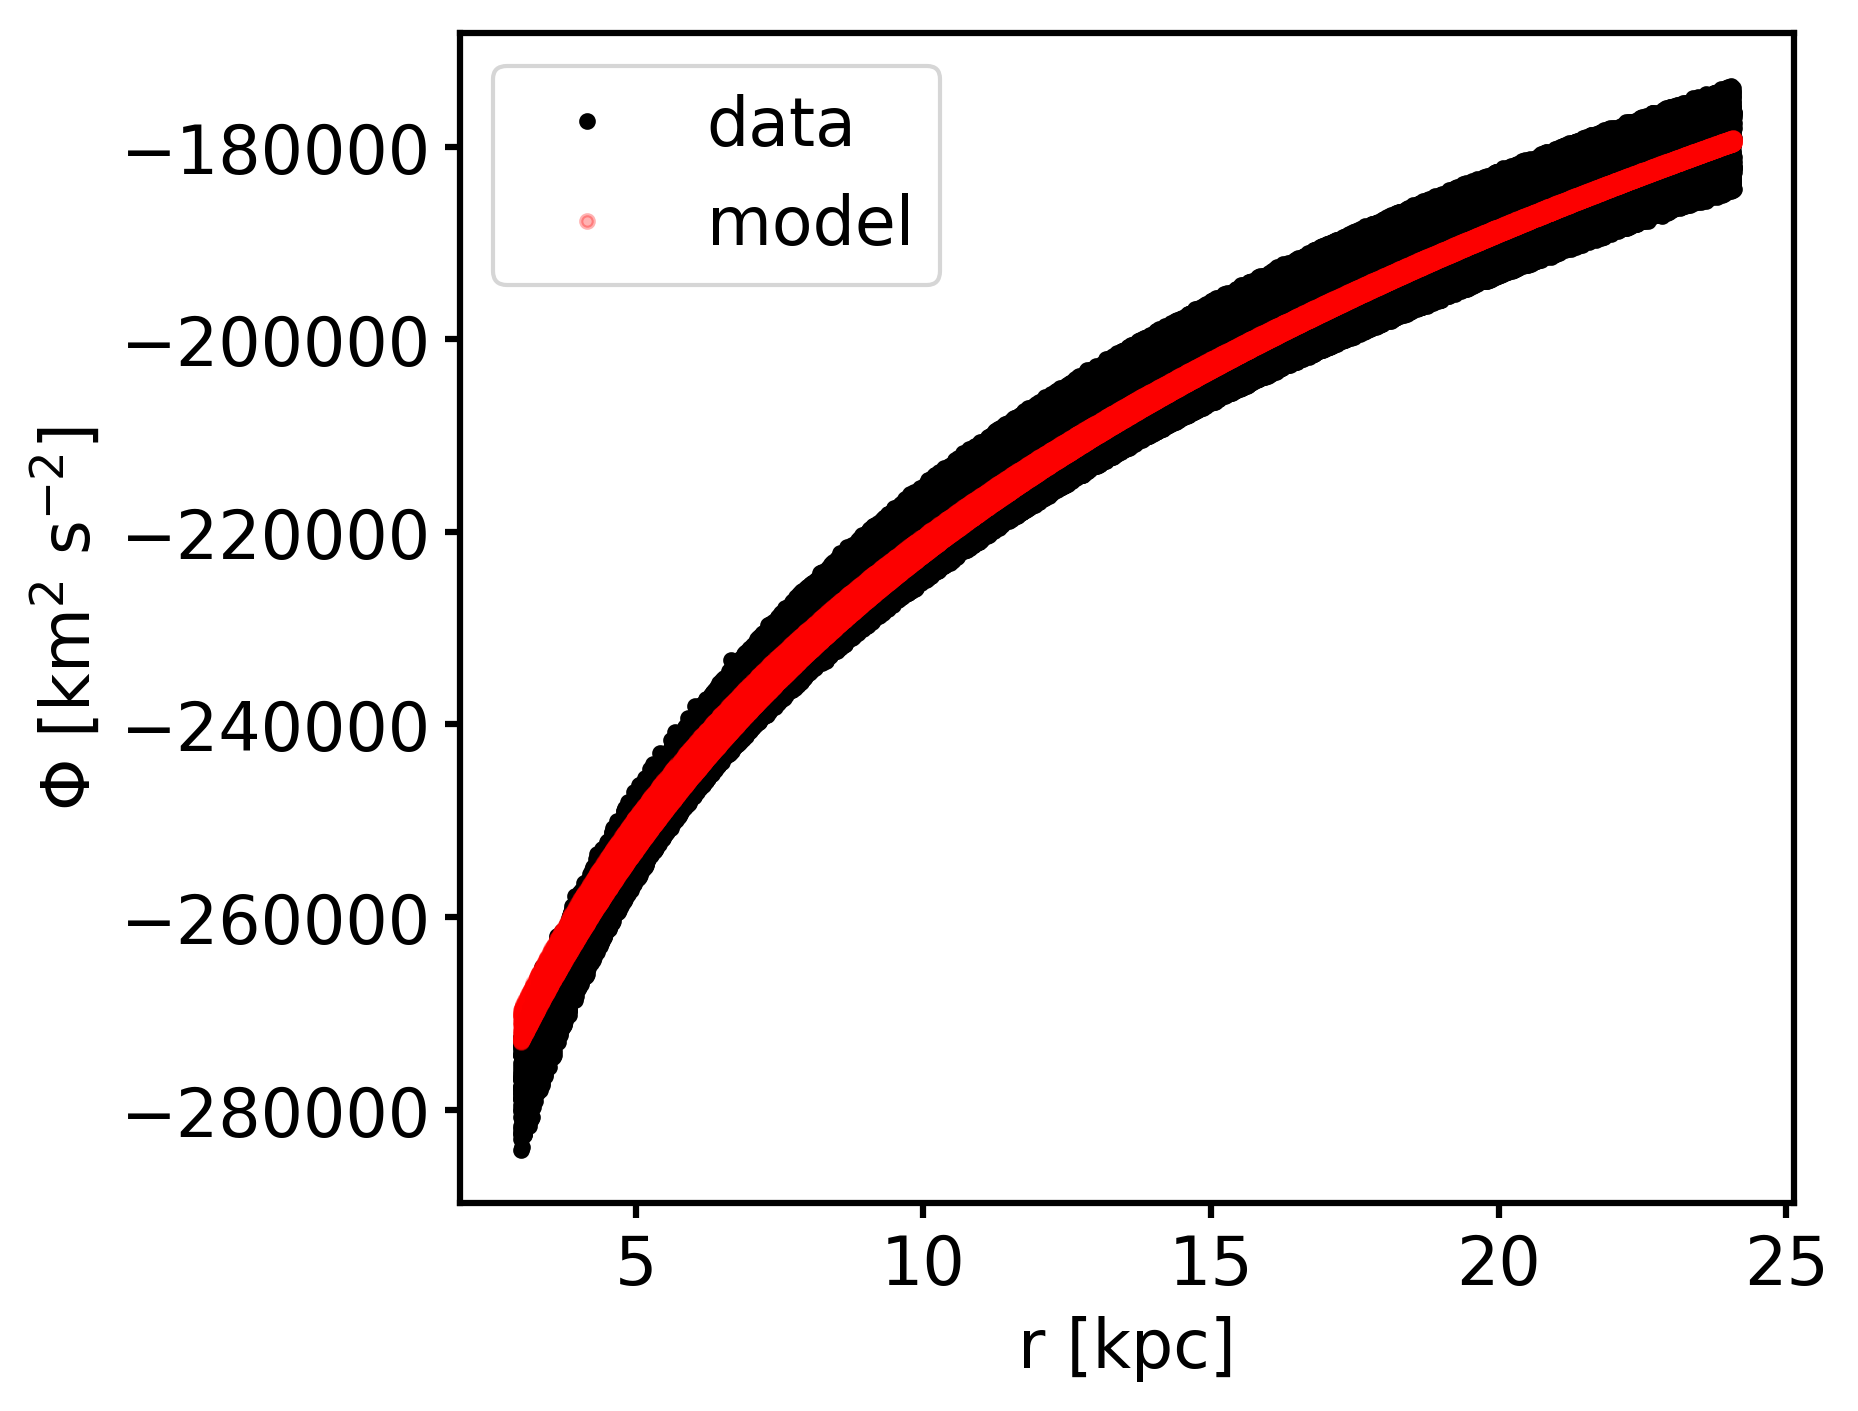
\includegraphics[width=0.7\textwidth]{plots/Auriga/phi_model_and_data_snap_127.png}
    \caption{Potential of data (selected \ac{DM} particles) and model depending on the radius r. Black dots are data, red dots from the best fit model. The innermost \SI{3}{kpc} are not included in the fit to make it better in the outer parts. The model lies everywhere within the data range but the slope seems less steep than the slope of the data.}
    \label{fig:potential_best_fit}
\end{SCfigure}
The result is shown in Figure \ref{fig:potential_best_fit} where we see the 'pot' value of the selected \ac{DM} particles in black and the fitted \ac{NFW} potential overlaying in red. Even though the red dots lie within the distribution of the black dots, the slope seems to be different. We find the best fit scale length of the \ac{DM} halo, $a_{\mathrm{NFWH}}$ as well as the total circular velocity $v_{0,\mathrm{tot}} \equiv v_{\mathrm{circ}}(R_0 = \SI{8}{kpc}) $. From that total circular velocity we can subtract the fraction from the stellar components to get the \ac{DM} component, $v_{0,\mathrm{NFWH}} = \sqrt{v_{0,\mathrm{tot}}^2 - v_{0, \mathrm{MND}}^2 - v_{0, \mathrm{HB}}^2}$. The resulting parameter values are summarized in Table \ref{tab:pot_best_fit_params}. 

\begin{figure}
\captionsetup{format=plain}
    \centering
    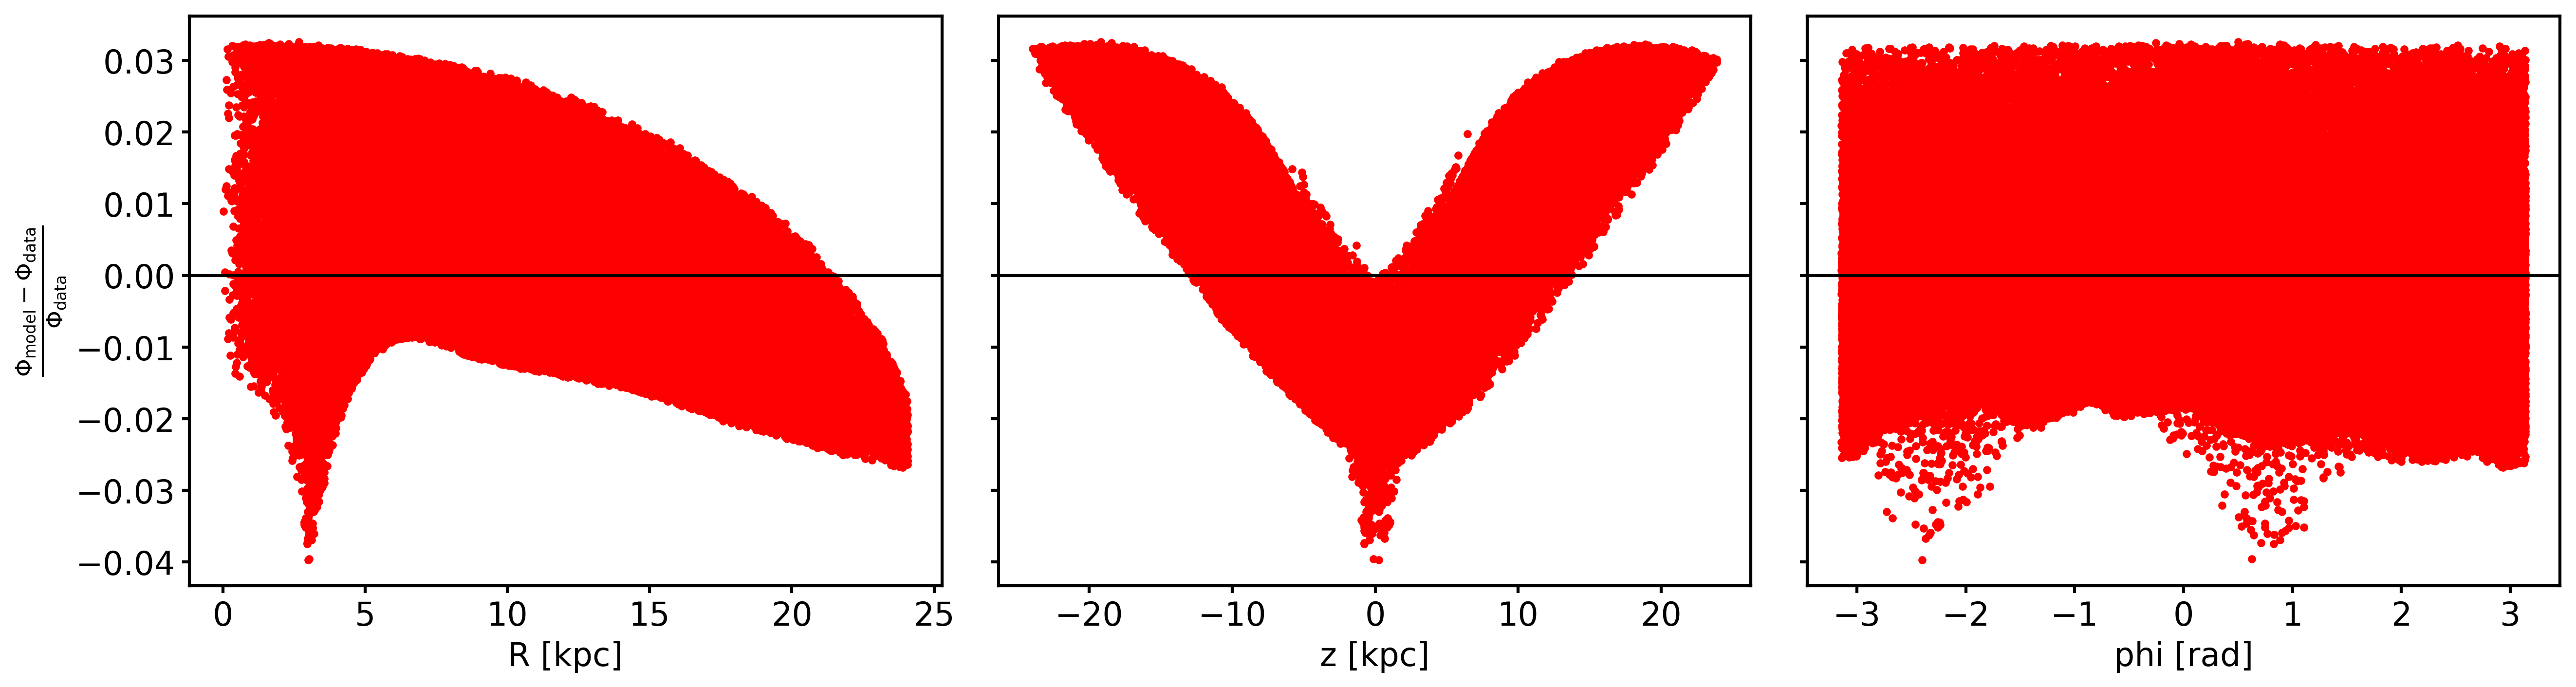
\includegraphics[width=\textwidth]{plots/Auriga/rel_phi_error_snap_127.png}
    \caption{Relative error $(\Phi_\mathrm{model} - \Phi_\mathrm{data})/\Phi_\mathrm{data})$ of the \ac{DM} fit versus the three cylindrical coordinates $(R, \phi, z)$. The errors are within a good range (3-4\%) but the slopes are not constant as they should. \textcolor{red}{update rel errors coming}}
    \label{fig:potential_fit_rel_errors}
\end{figure}
To check, how good the slope of the \ac{DM} fit is, we plot the relative error $(\Phi_\mathrm{model} - \Phi_\mathrm{data})/\Phi_\mathrm{data})$ versus the three cylindrical coordinates $(R, \phi, z)$. The slopes should be constant which they are not. We tried many different routines for the potential fit and this is the best we got and since the errors are relatively small (within 3-4\%) we still think the fit is good enough.

\subsubsection{Total potential}\label{subsubsec:tot_pot}
After fitting each component individually, we add them up to get a total potential.
\begin{table}[htbp]
\captionsetup{format=plain}
    \centering
    \begin{tabular}{@{}llll@{}}
         \toprule
         component& potential & parameters \& values &fitting method  \\
         \midrule
         stellar disk& \makecell[tl]{Miyamoto\\-Nagai}&\makecell[tl]{$a_{\mathrm{MND}}$ = \SI{2.97}{kpc}\\$b_{\mathrm{MND}}$ = \SI{1.64}{kpc}\\$v_{0,\mathrm{MND}}$ = \SI{105.00}{km.s^{-1}}} & \makecell[tl]{\ac{MN} density fitted \\to density bins \\of disk in $(R,z)$.}\vspace{3mm}\\
         %\midrule
         \makecell[tl]{stellar\\ spheroid}& Hernquist&\makecell[tl]{$a_{\mathrm{HB}}$ = \SI{1.82}{kpc}\\$v_{0,\mathrm{HB}}$ = \SI{110.00}{km.s^{-1}}}& \makecell[tl]{Hernquist density fitted\\ to density shells of \\spheroid in $(r)$.}\vspace{3mm}\\
         %\midrule
         \ac{DM} halo&\ac{NFW}&\makecell[tl]{$a_{\mathrm{NFWH}}$ = \SI{25.47}{kpc}\\$v_{0,\mathrm{NFWH}}$ = \SI{160.66}{km.s^{-1}}}&\makecell[tl]{Total potential fitted to \\'pot' value of random \ac{DM} \\particles where \ac{NFW}\\ parameters were fitting \\parameters.}\vspace{3mm}\\
         %\midrule
         total & \makecell[tl]{sum of these\\ potentials} & \makecell[tl]{$R_0$ = \SI{8.00}{kpc} \\ $v_{0,\mathrm{tot}}$ = \SI{221.21}{km.s^{-1}}}& \makecell[tl]{$v_0$ is the total circular \\ velocity at $R_0$.}\vspace{3mm}\\
         \bottomrule 
    \end{tabular}
    \caption{Best fit potential overview: components, used potentials, their parameters with best fit values and their fitting methods. \textcolor{red}{update absolute error and hist2d coming}}
    \label{tab:pot_best_fit_params}
\end{table}
In Table \ref{tab:pot_best_fit_params}, we summarize our results for the last snapshot as described in the previous Sections. 
 
\begin{table}[htbp]
\captionsetup{format=plain}
    \centering
    \begin{tabular}{@{}lllll@{}}
         \toprule
         Quantity & Unit& \makecell[tr]{This work} & \makecell[tr]{Auriga \\\citetalias{AurigaGrand} }&\makecell[tr]{Milky Way\\ \citetalias{Bland-Hawthorn...MW...2016}}\\
         \midrule
         \makecell[tl]{Disk scale length}& [kpc] & \makecell[tr]{2.97}&\makecell[tr]{5.57} & \makecell[tr]{$2.6\pm0.5$ \\(thin disk)}\\
         \makecell[tl]{Bulge scale length}& [kpc] & \makecell[tr]{1.82}&\makecell[tr]{0.95} & \makecell[tr]{$1.9-2.8$ \\\citetalias{Vanhollebeke...bulge...2009}}\\
         \makecell[tl]{\ac{DM} halo scale length}& [kpc] & \makecell[tr]{25.47}&\makecell[tr]{none} & \makecell[tr]{$25 \pm 10 $}\vspace{3mm}\\
         \makecell[tl]{Disk mass \\ within $0.1R_{200}$} & [$10^{10}\mathrm{M}_\odot$] &  \makecell[tr]{}&\makecell[tr]{3.76} & \makecell[tr]{$3.5\pm1$\\(thin disk)}\\
         \makecell[tl]{Bulge mass \\ within $0.1R_{200} $}& [$10^{10}\mathrm{M}_\odot$] &\makecell[tr]{} &\makecell[tr]{2.19}& \makecell[tr]{$1.4-1.7$}\\
         \makecell[tl]{Total stellar mass \\ within $0.1R_{200}$ }& [$10^{10}\mathrm{M}_\odot$] & \makecell[tr]{} &\makecell[tr]{6.55}& \makecell[tr]{$5 \pm 1$}\\
         \makecell[tl]{\ac{D/T}} & & \makecell[tr]{0.47}&\makecell[tr]{0.63} & \makecell[tr]{0.7 \\(thin disk)}\vspace{3mm}\\ 
         %\midrule
         \makecell[tl]{$R_{200}=R(\rho = 200 \rho_\mathrm{crit}$)} & [kpc] &\makecell[tr]{240.86}  & \makecell[tr]{240.86} & \makecell[tr]{$209 \pm 23$}\\
         \makecell[tl]{$M_{200}=M(\rho = 200 \rho_\mathrm{crit})$} & [$10^{12}\mathrm{M}_\odot$] & \makecell[tr]{149.18}  & \makecell[tr]{149.18} & \makecell[tr]{$1.1 \pm 0.3$}\vspace{3mm}\\
         %\midrule
         \makecell[tl]{total circular velocity\\ at $R_0 = \SI{8}{kpc}$}&  [$\mathrm{km\ s}^{-1}$]& \makecell[tr]{221.21} & \makecell[tr]{none \\explicitly}& \makecell[tr]{$238 \pm 15$}\vspace{3mm}\\
         \bottomrule 
    \end{tabular}
    \caption{Comparison of some of the structural parameters of our results with the Auriga \citep{AurigaGrand} analysis and \ac{MW} values taken from \citet{Bland-Hawthorn...MW...2016}.}
    \label{tab:disk_quant_comparison}
\end{table}




\iffalse
\begin{figure}
\captionsetup{format=plain}
    \centering
    \begin{subfigure}[b]{0.3\textwidth}
	    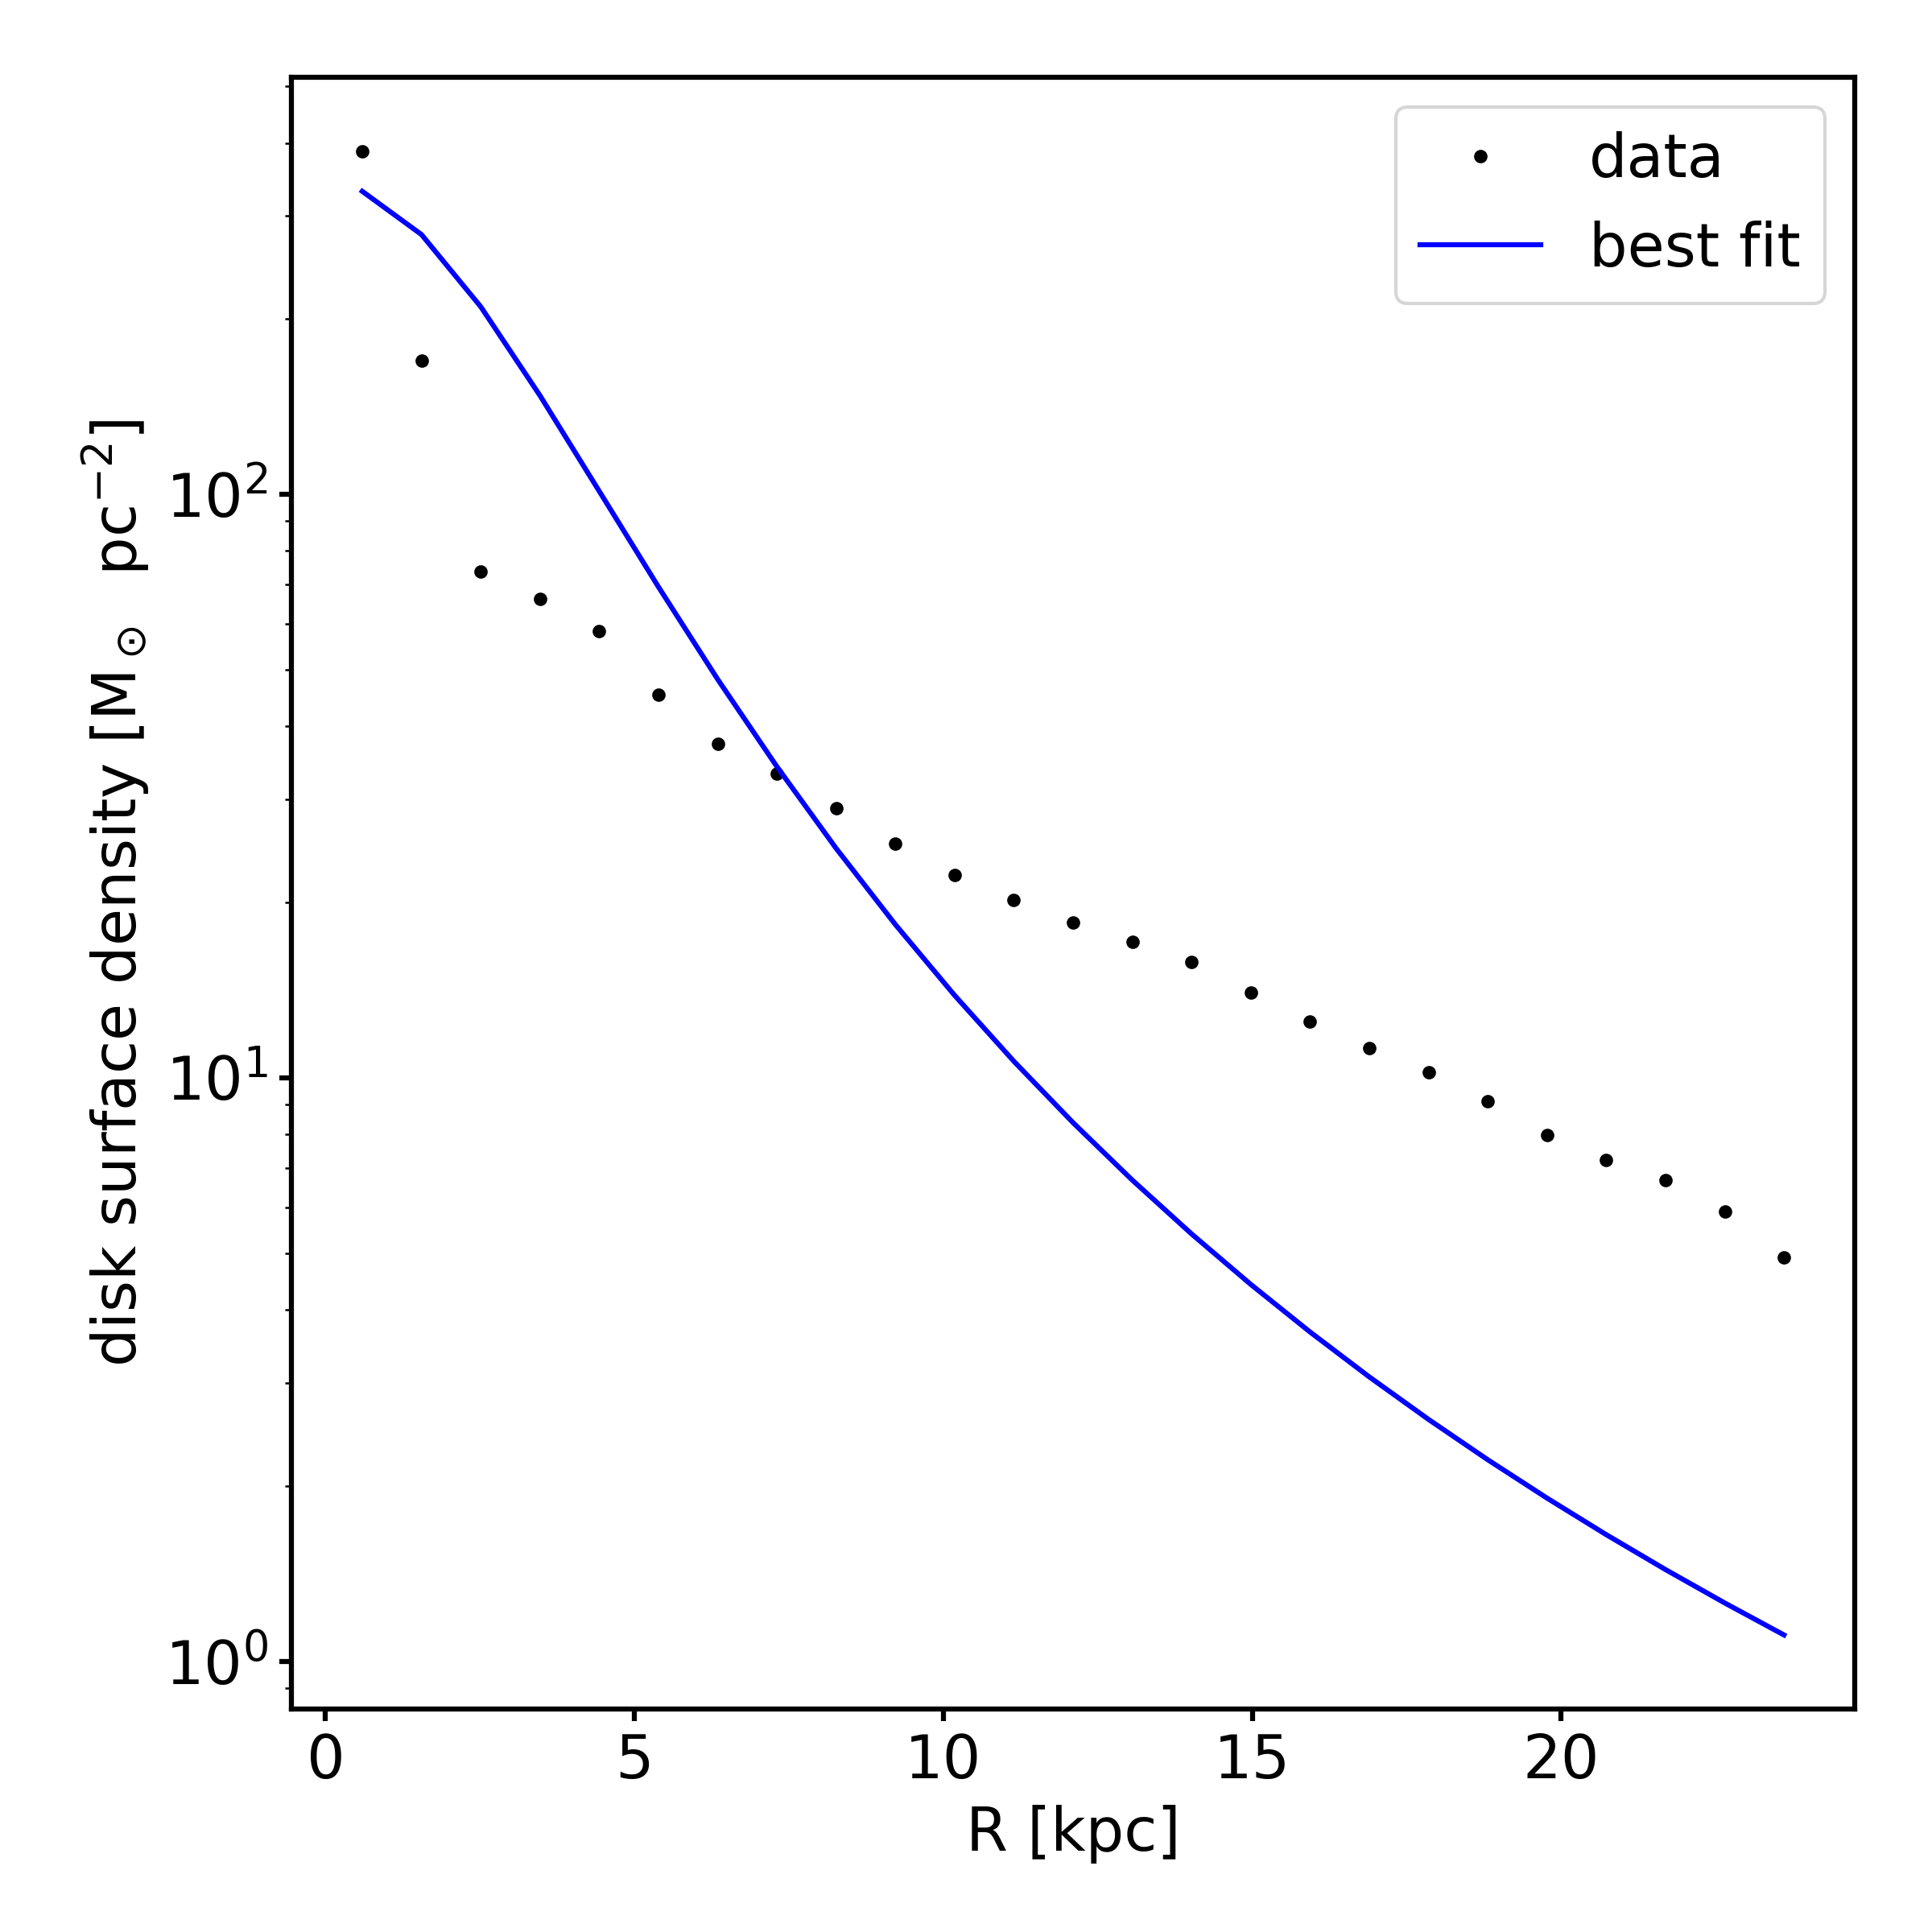
\includegraphics[width=\textwidth]{plots/Auriga/surface_dens_disk_fit_data.png}
	    \label{fig:disk_surfdens_fit}
    \end{subfigure}
    ~ %add desired spacing between images, e. g. ~, \quad, \qquad, \hfill etc. 
      %(or a blank line to force the subfigure onto a new line)
    \begin{subfigure}[b]{0.3\textwidth}
    \centering
    	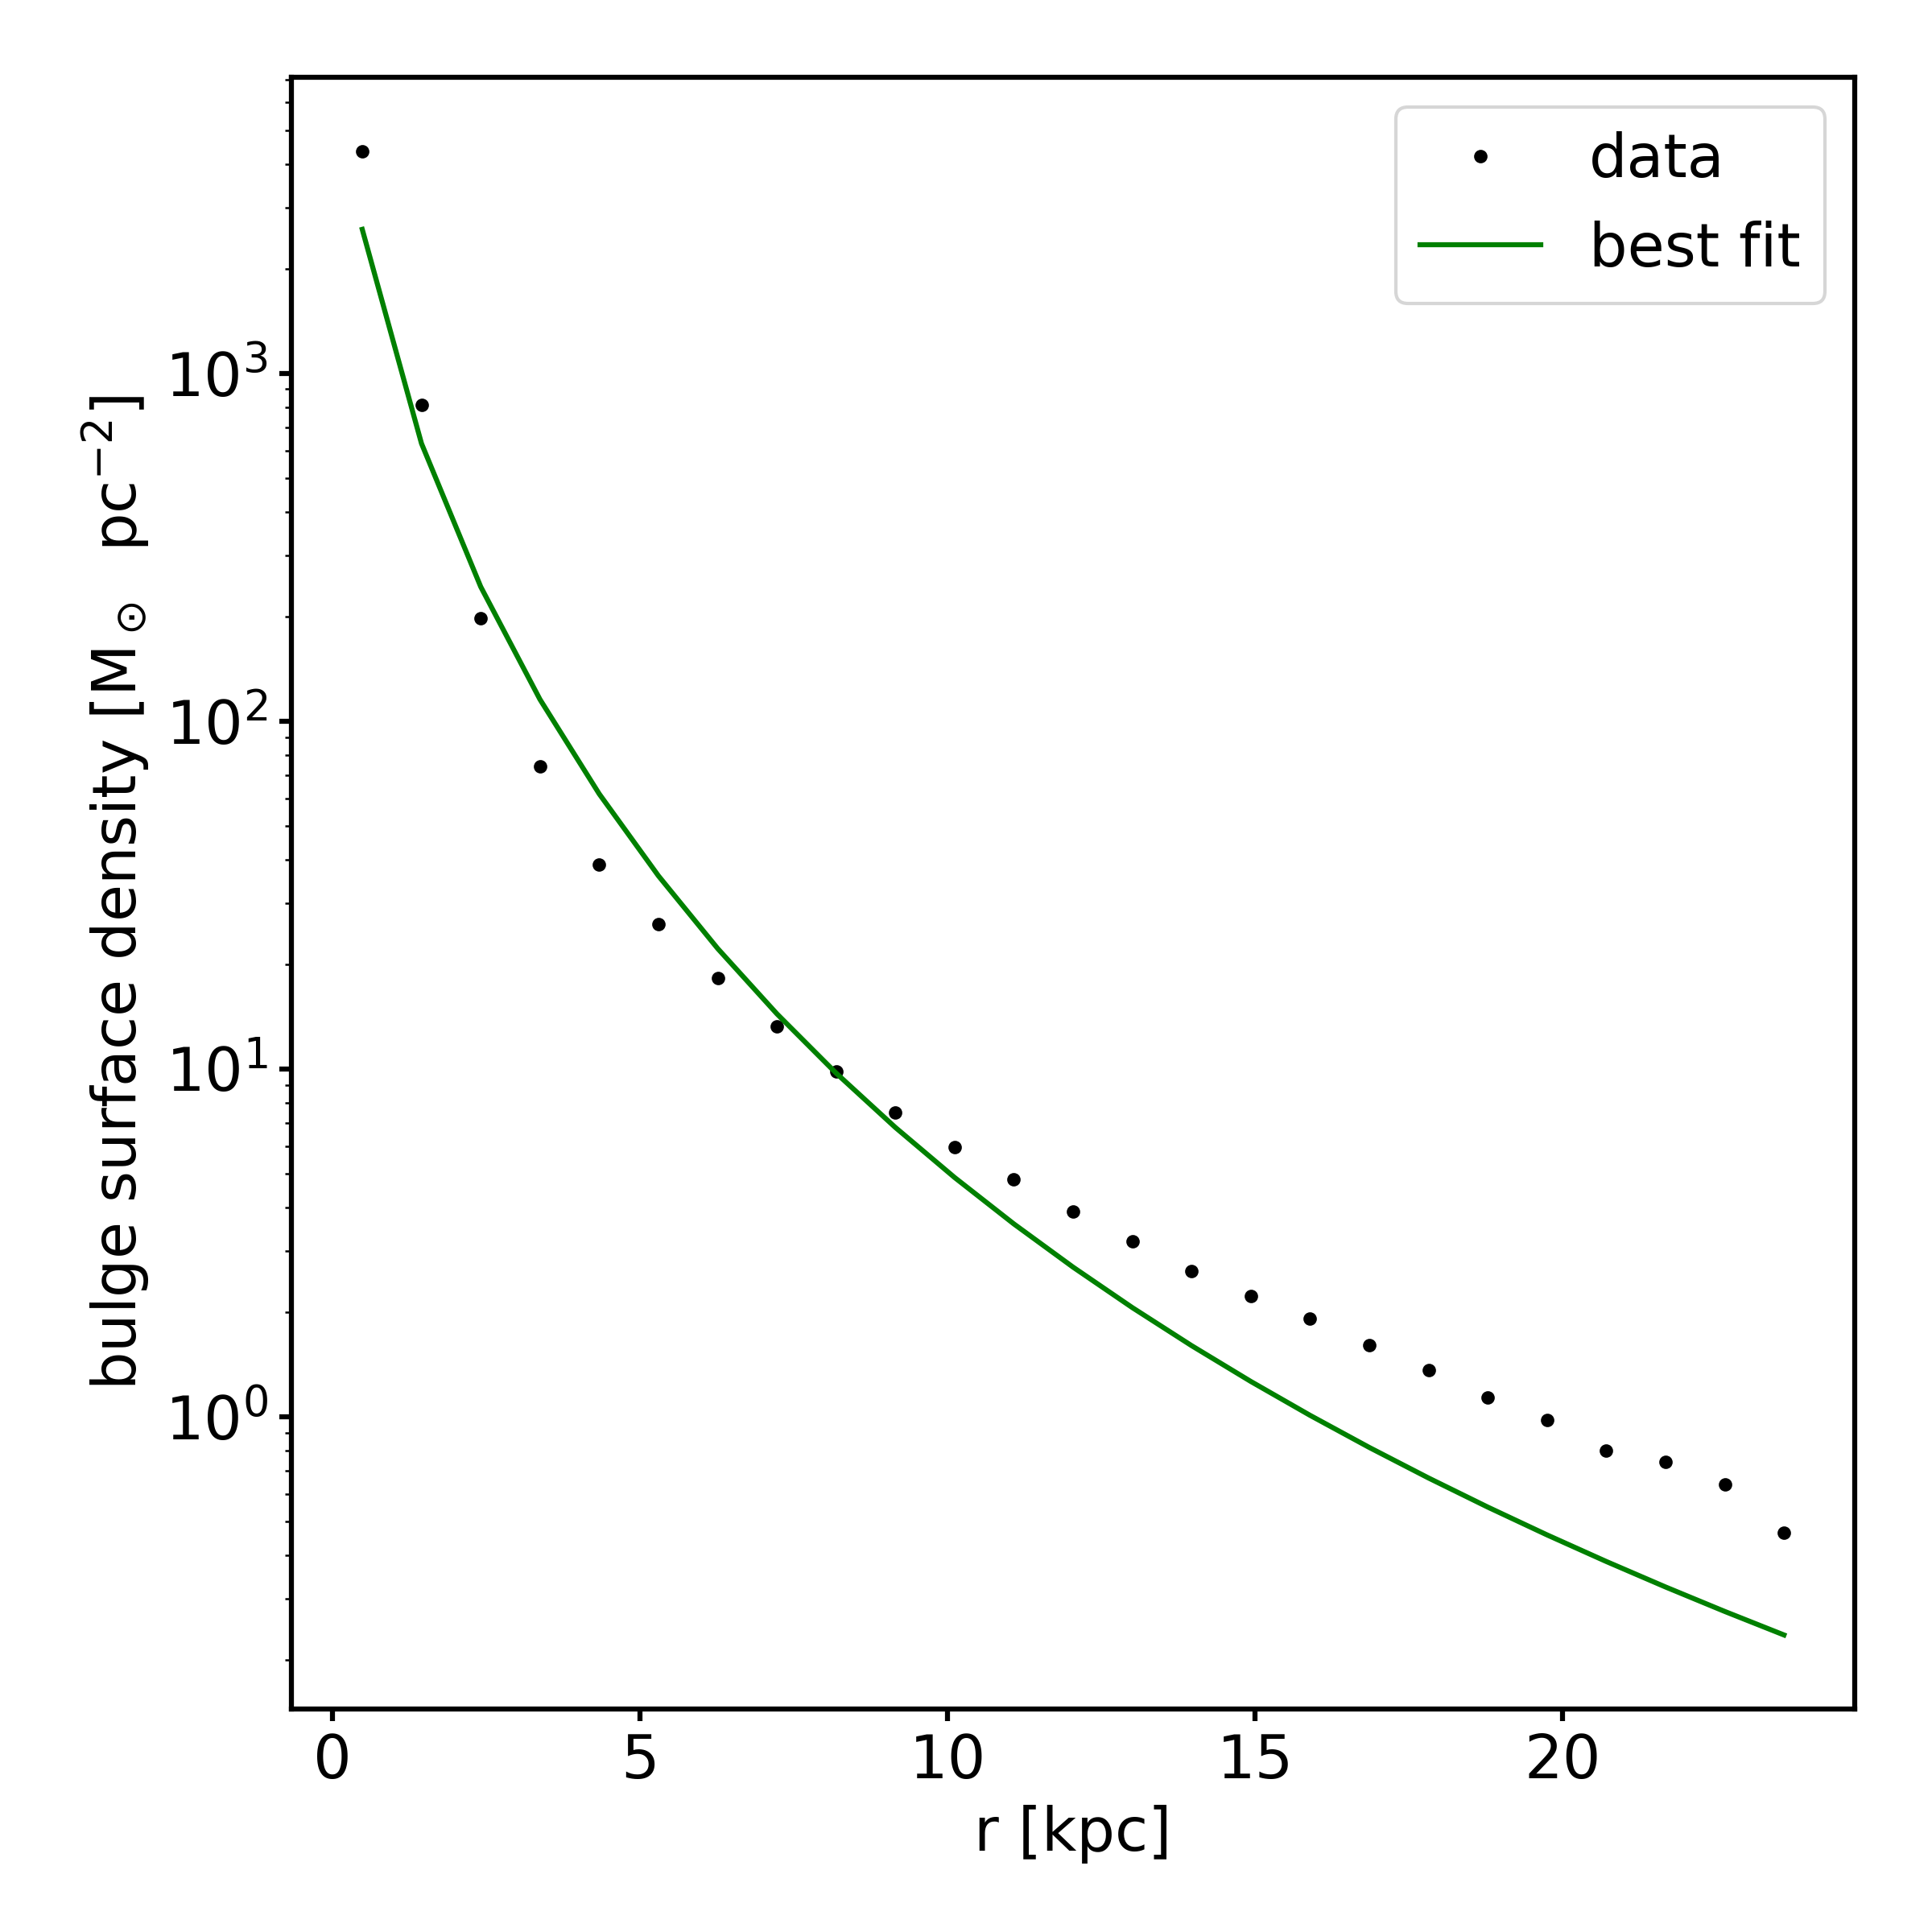
\includegraphics[width=\textwidth]{plots/Auriga/surface_dens_spher_fit_data.png}
    	\label{fig:spher_surfdens_fit}
    \end{subfigure}
    ~ %add desired spacing between images, e. g. ~, \quad, \qquad, \hfill etc. 
    %(or a blank line to force the subfigure onto a new line)
    \begin{subfigure}[b]{0.3\textwidth}
    \centering
    	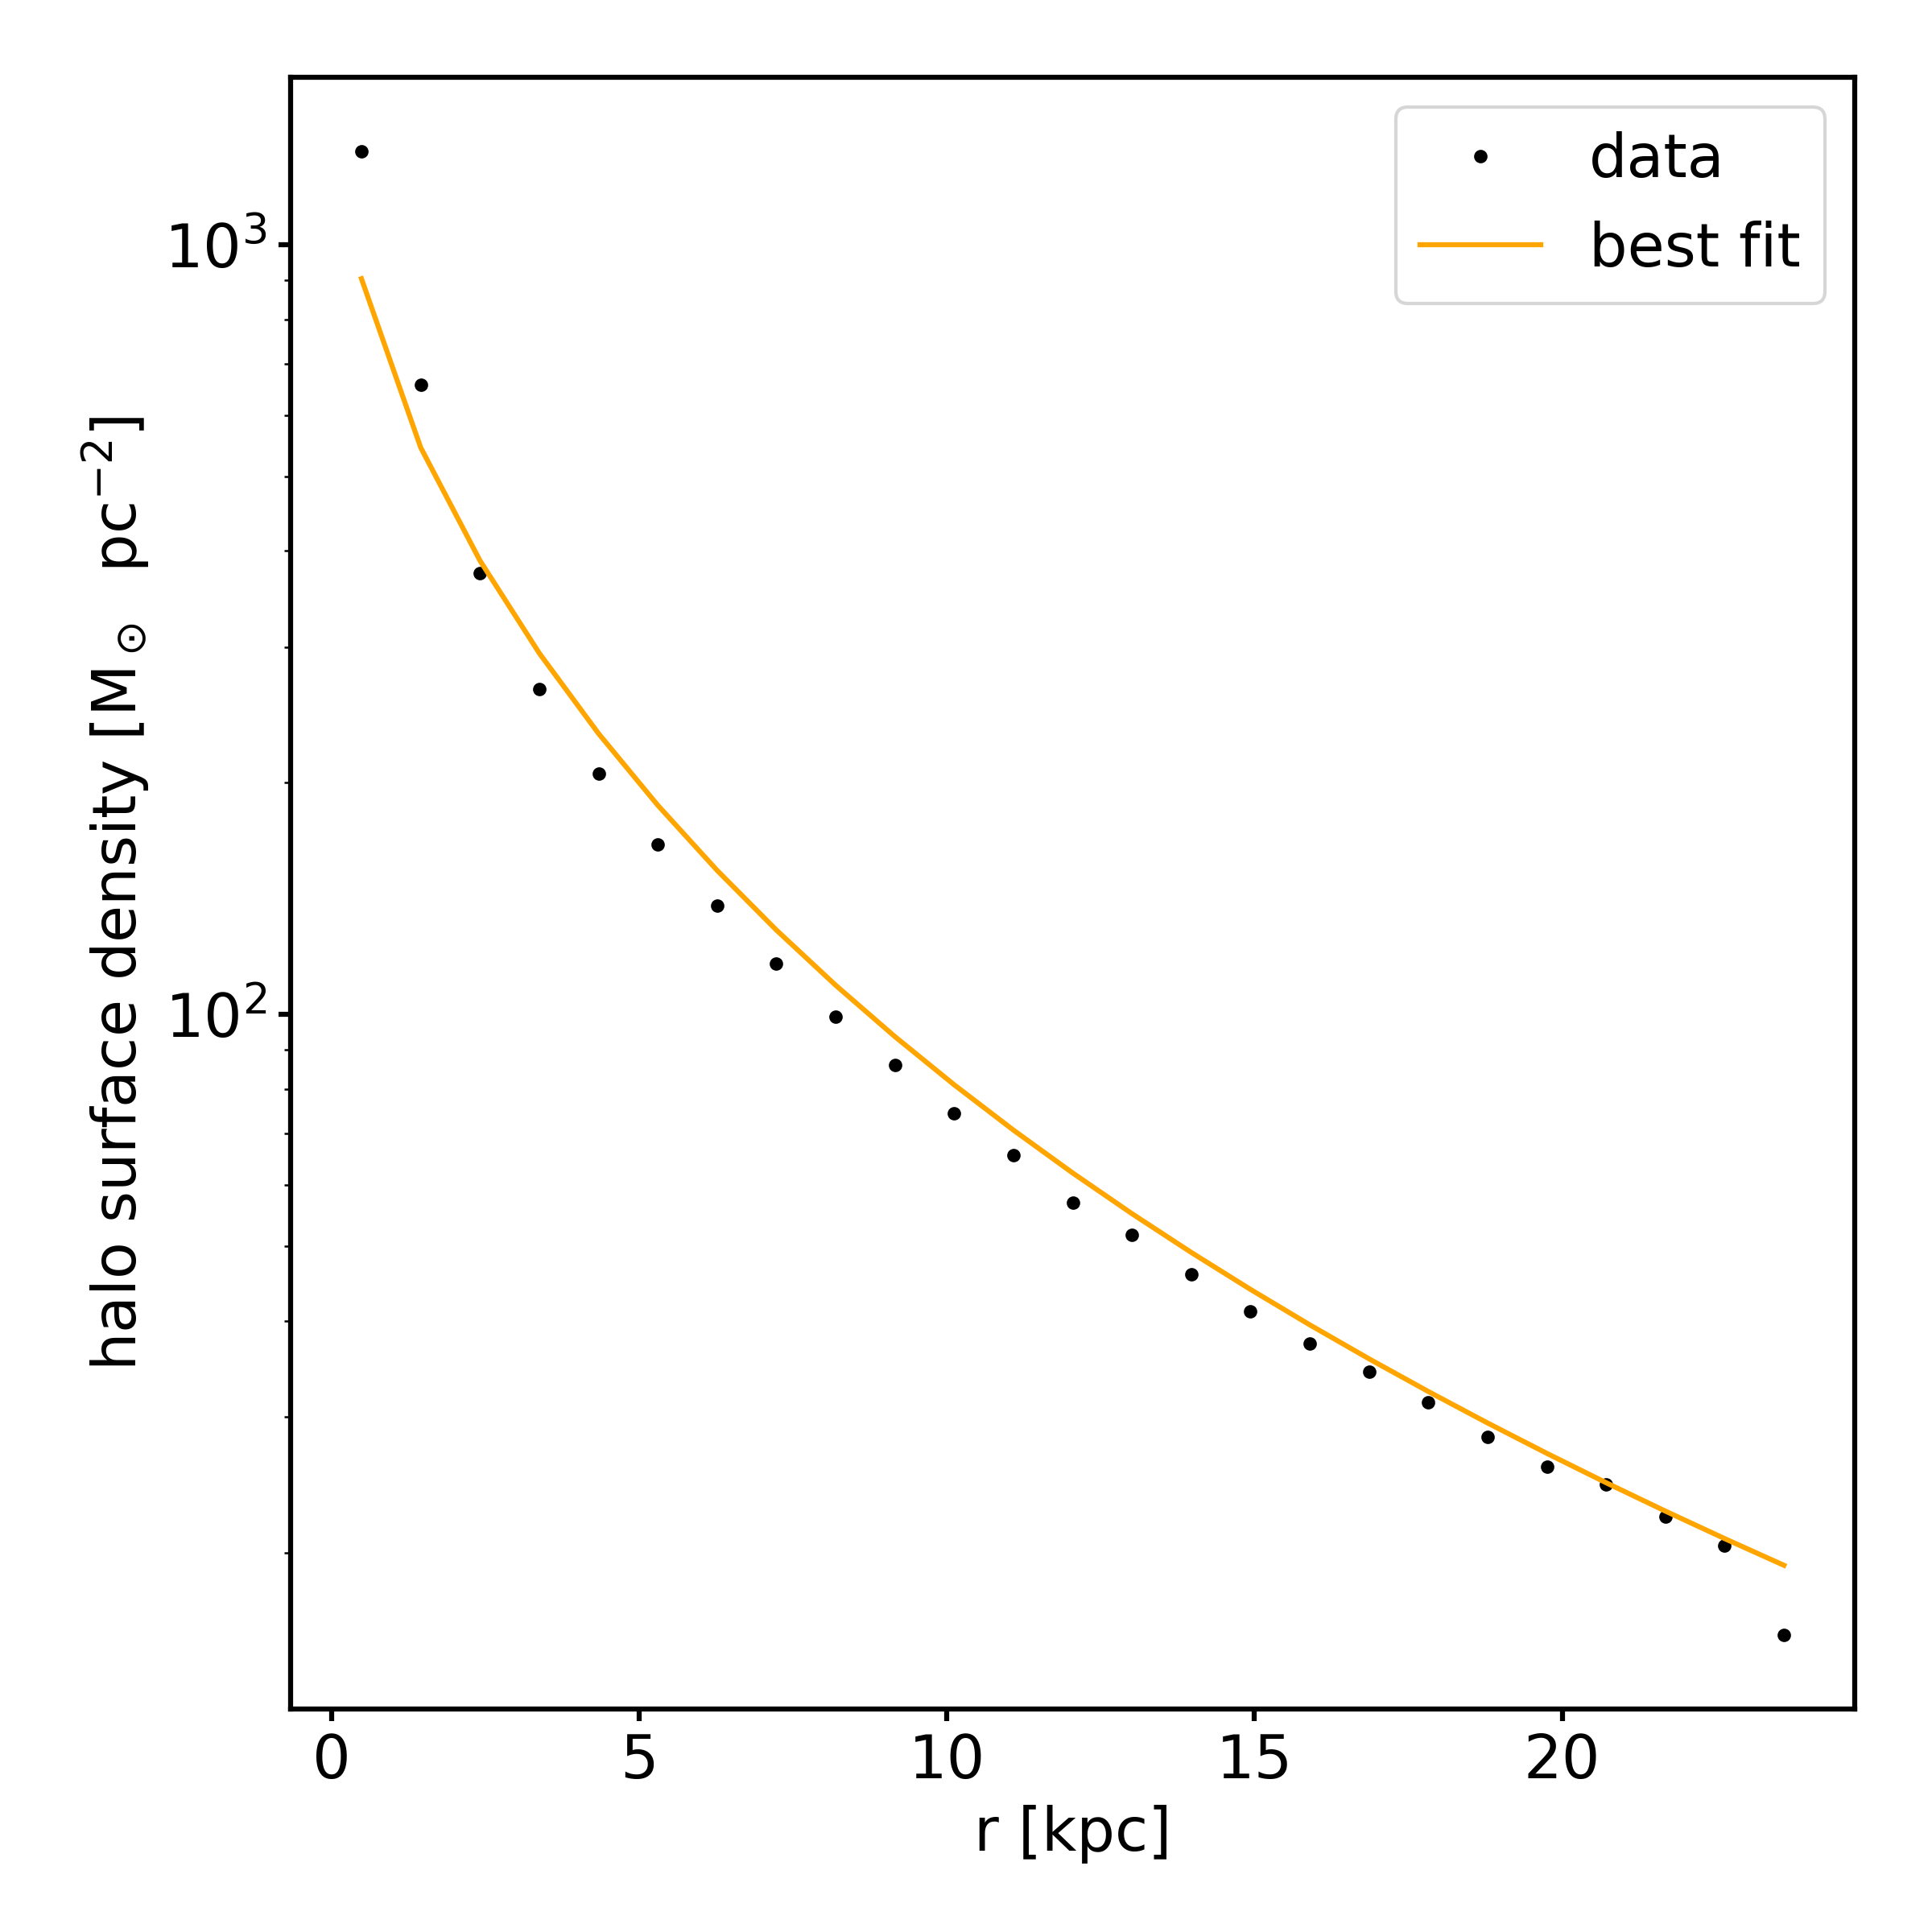
\includegraphics[width=\textwidth]{plots/Auriga/surface_dens_halo_fit_data.png}
    	\label{fig:halo_surfdens_fit}
    \end{subfigure}
    
    \begin{subfigure}[b]{0.3\textwidth}
        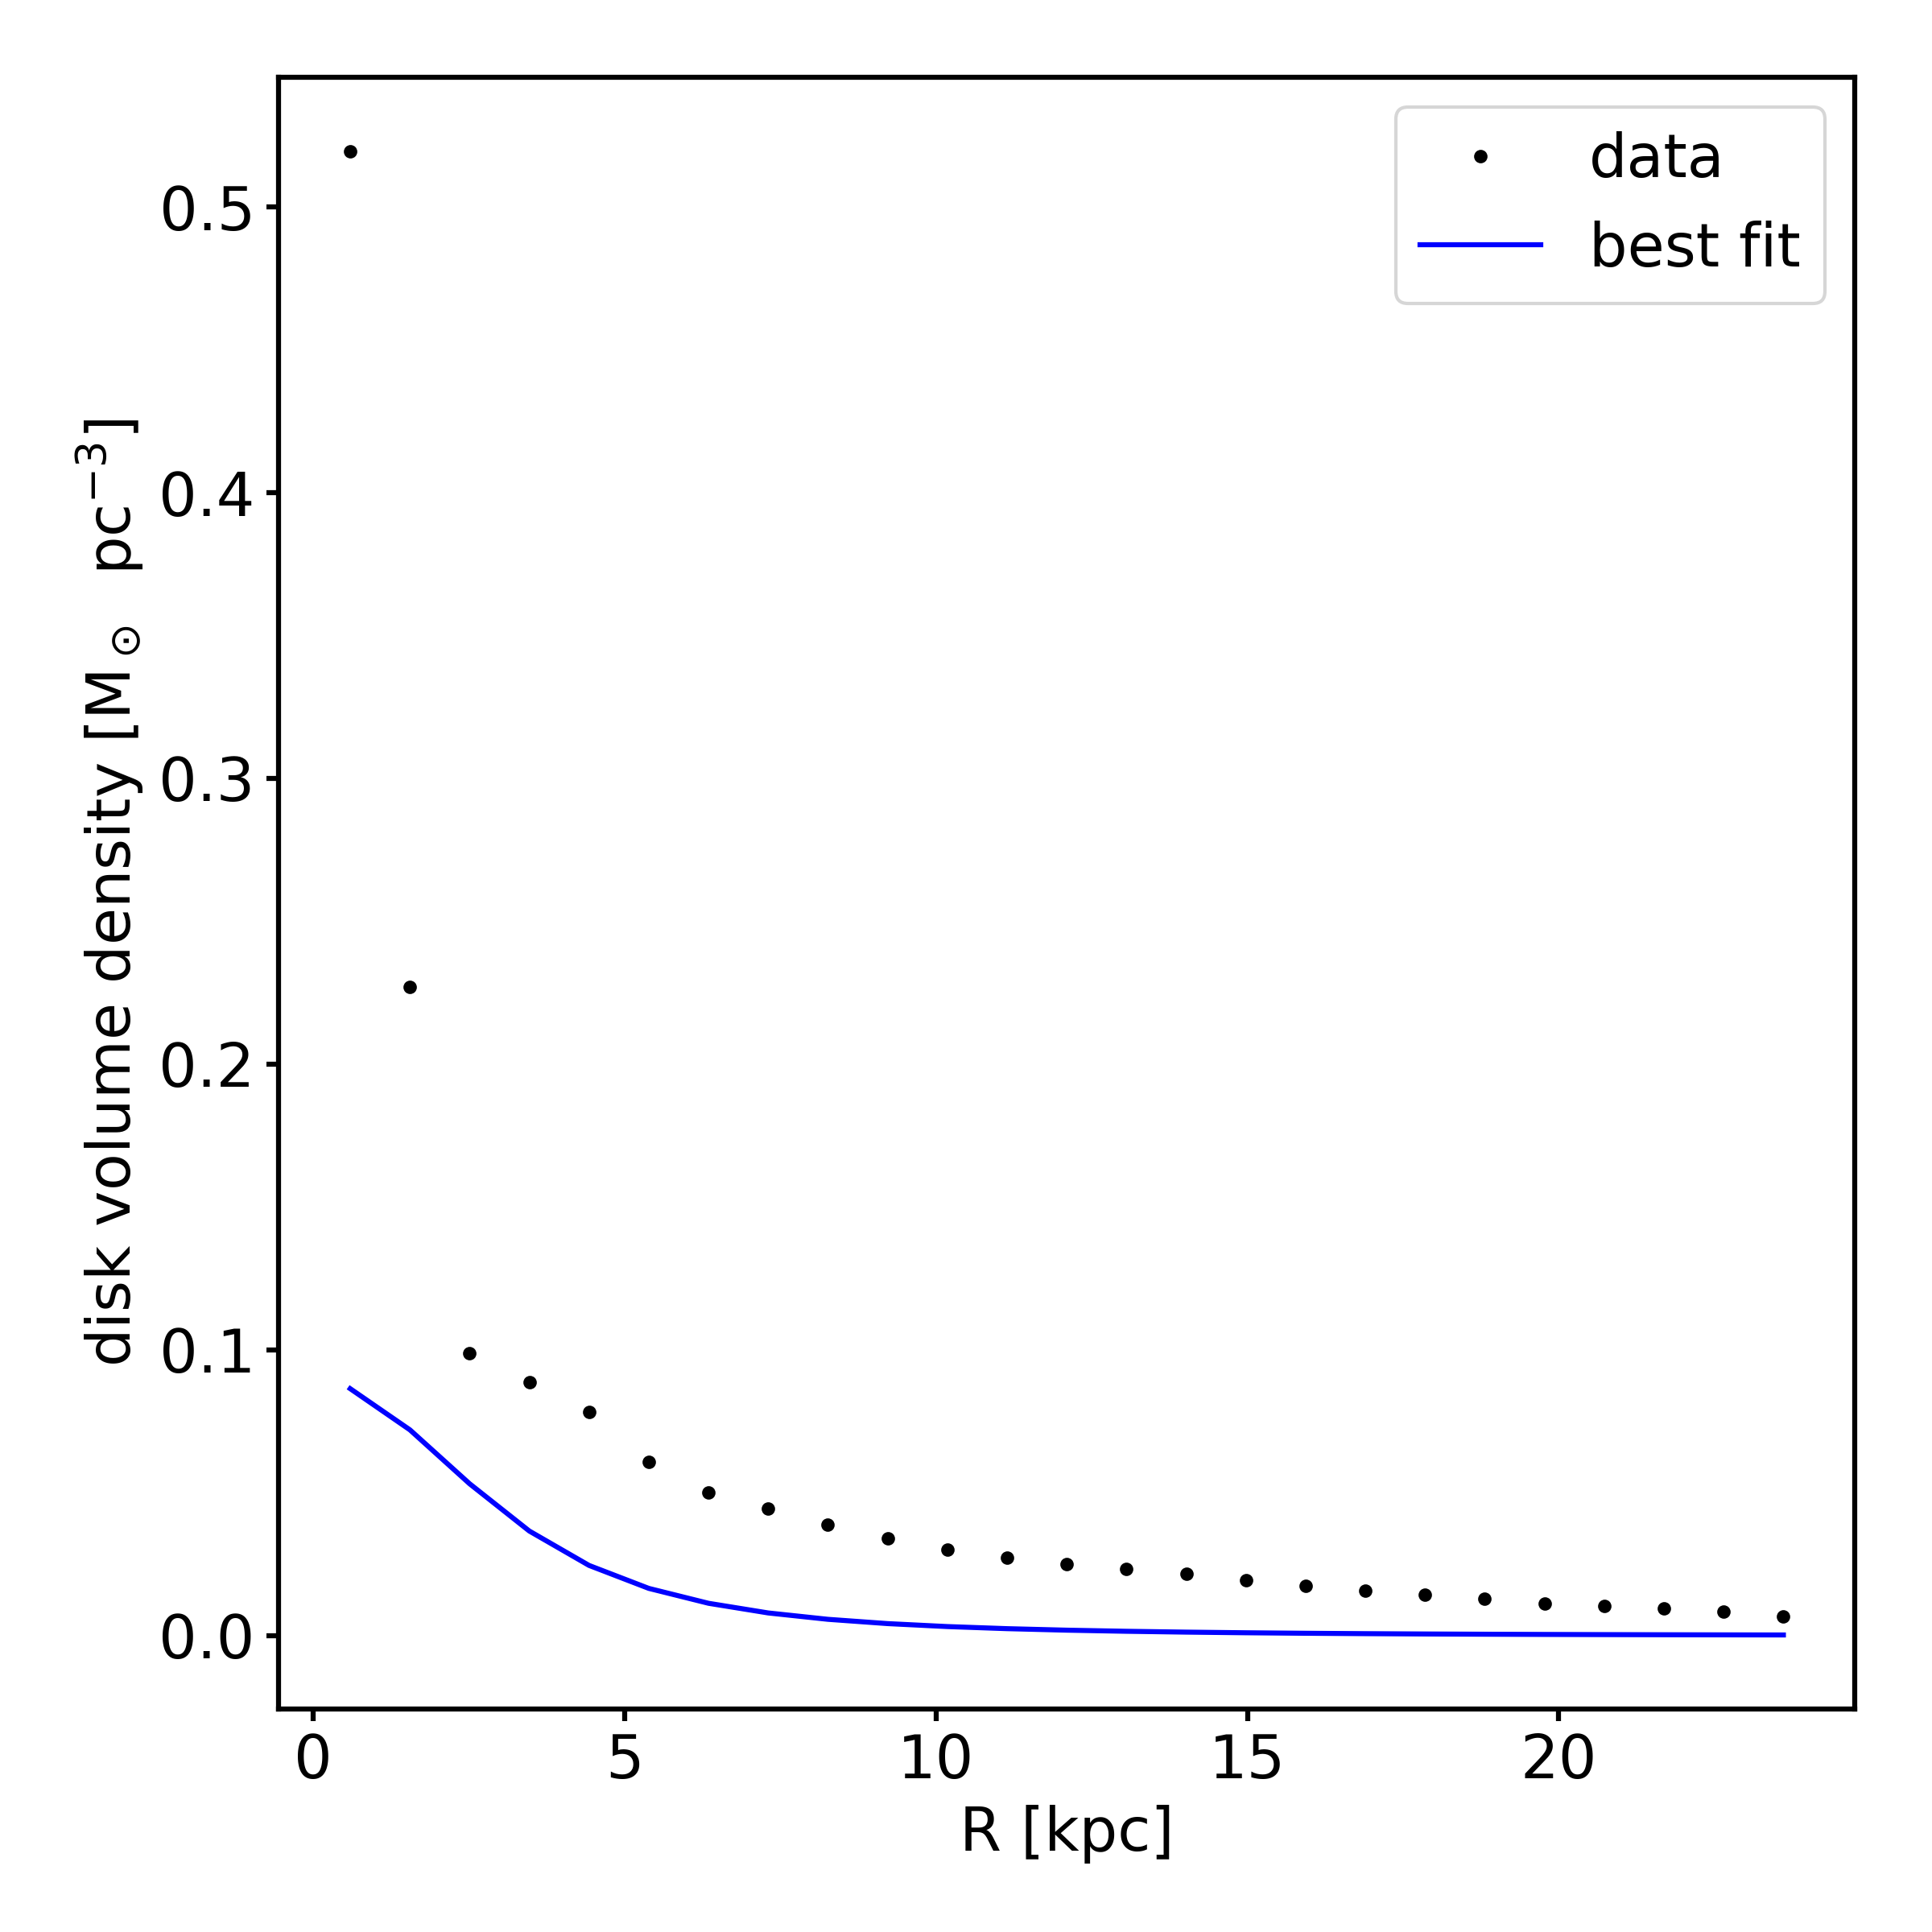
\includegraphics[width=\textwidth]{plots/Auriga/volume_dens_disk_fit_data.png}
	    \label{fig:disk_voldens_fit}
    \end{subfigure}
    ~ %add desired spacing between images, e. g. ~, \quad, \qquad, \hfill etc. 
    %(or a blank line to force the subfigure onto a new line)
    \begin{subfigure}[b]{0.3\textwidth}
    \centering
    	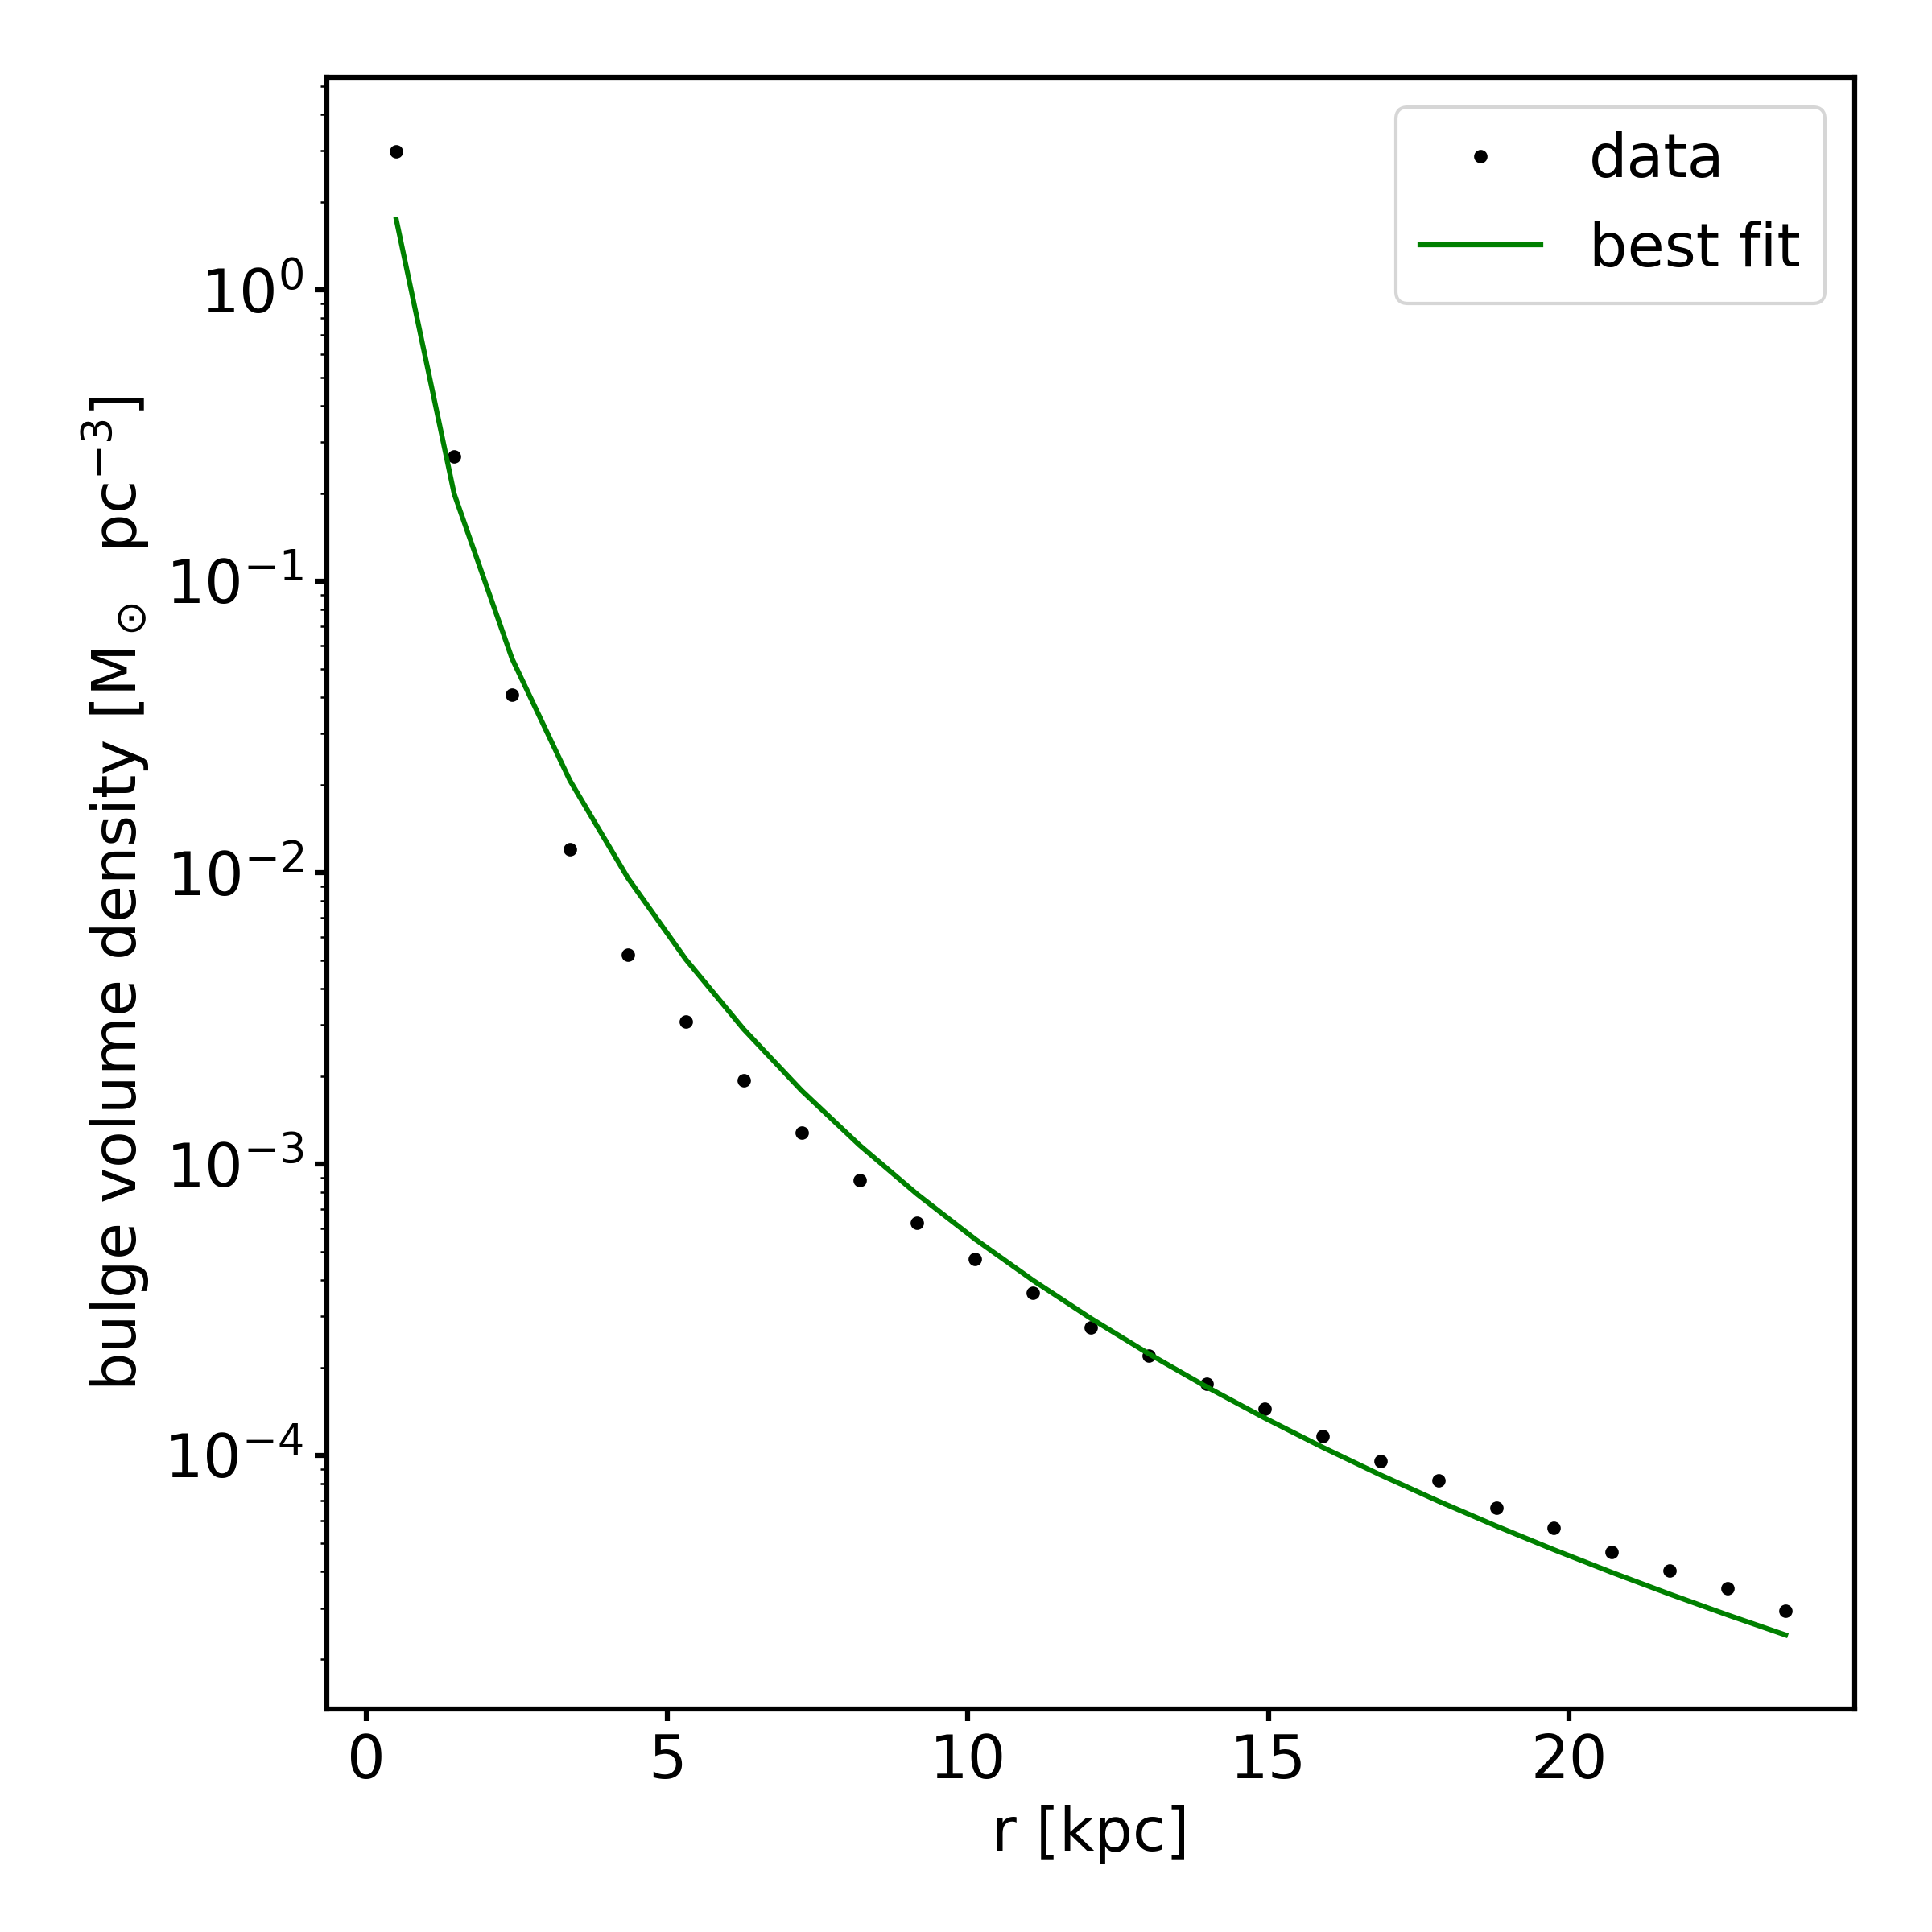
\includegraphics[width=\textwidth]{plots/Auriga/volume_dens_bulge_fit_data.png}
    	\label{fig:spher_voldens_fit}
    \end{subfigure}
    ~ %add desired spacing between images, e. g. ~, \quad, \qquad, \hfill etc. 
    %(or a blank line to force the subfigure onto a new line)
    \begin{subfigure}[b]{0.3\textwidth}
        \centering
    	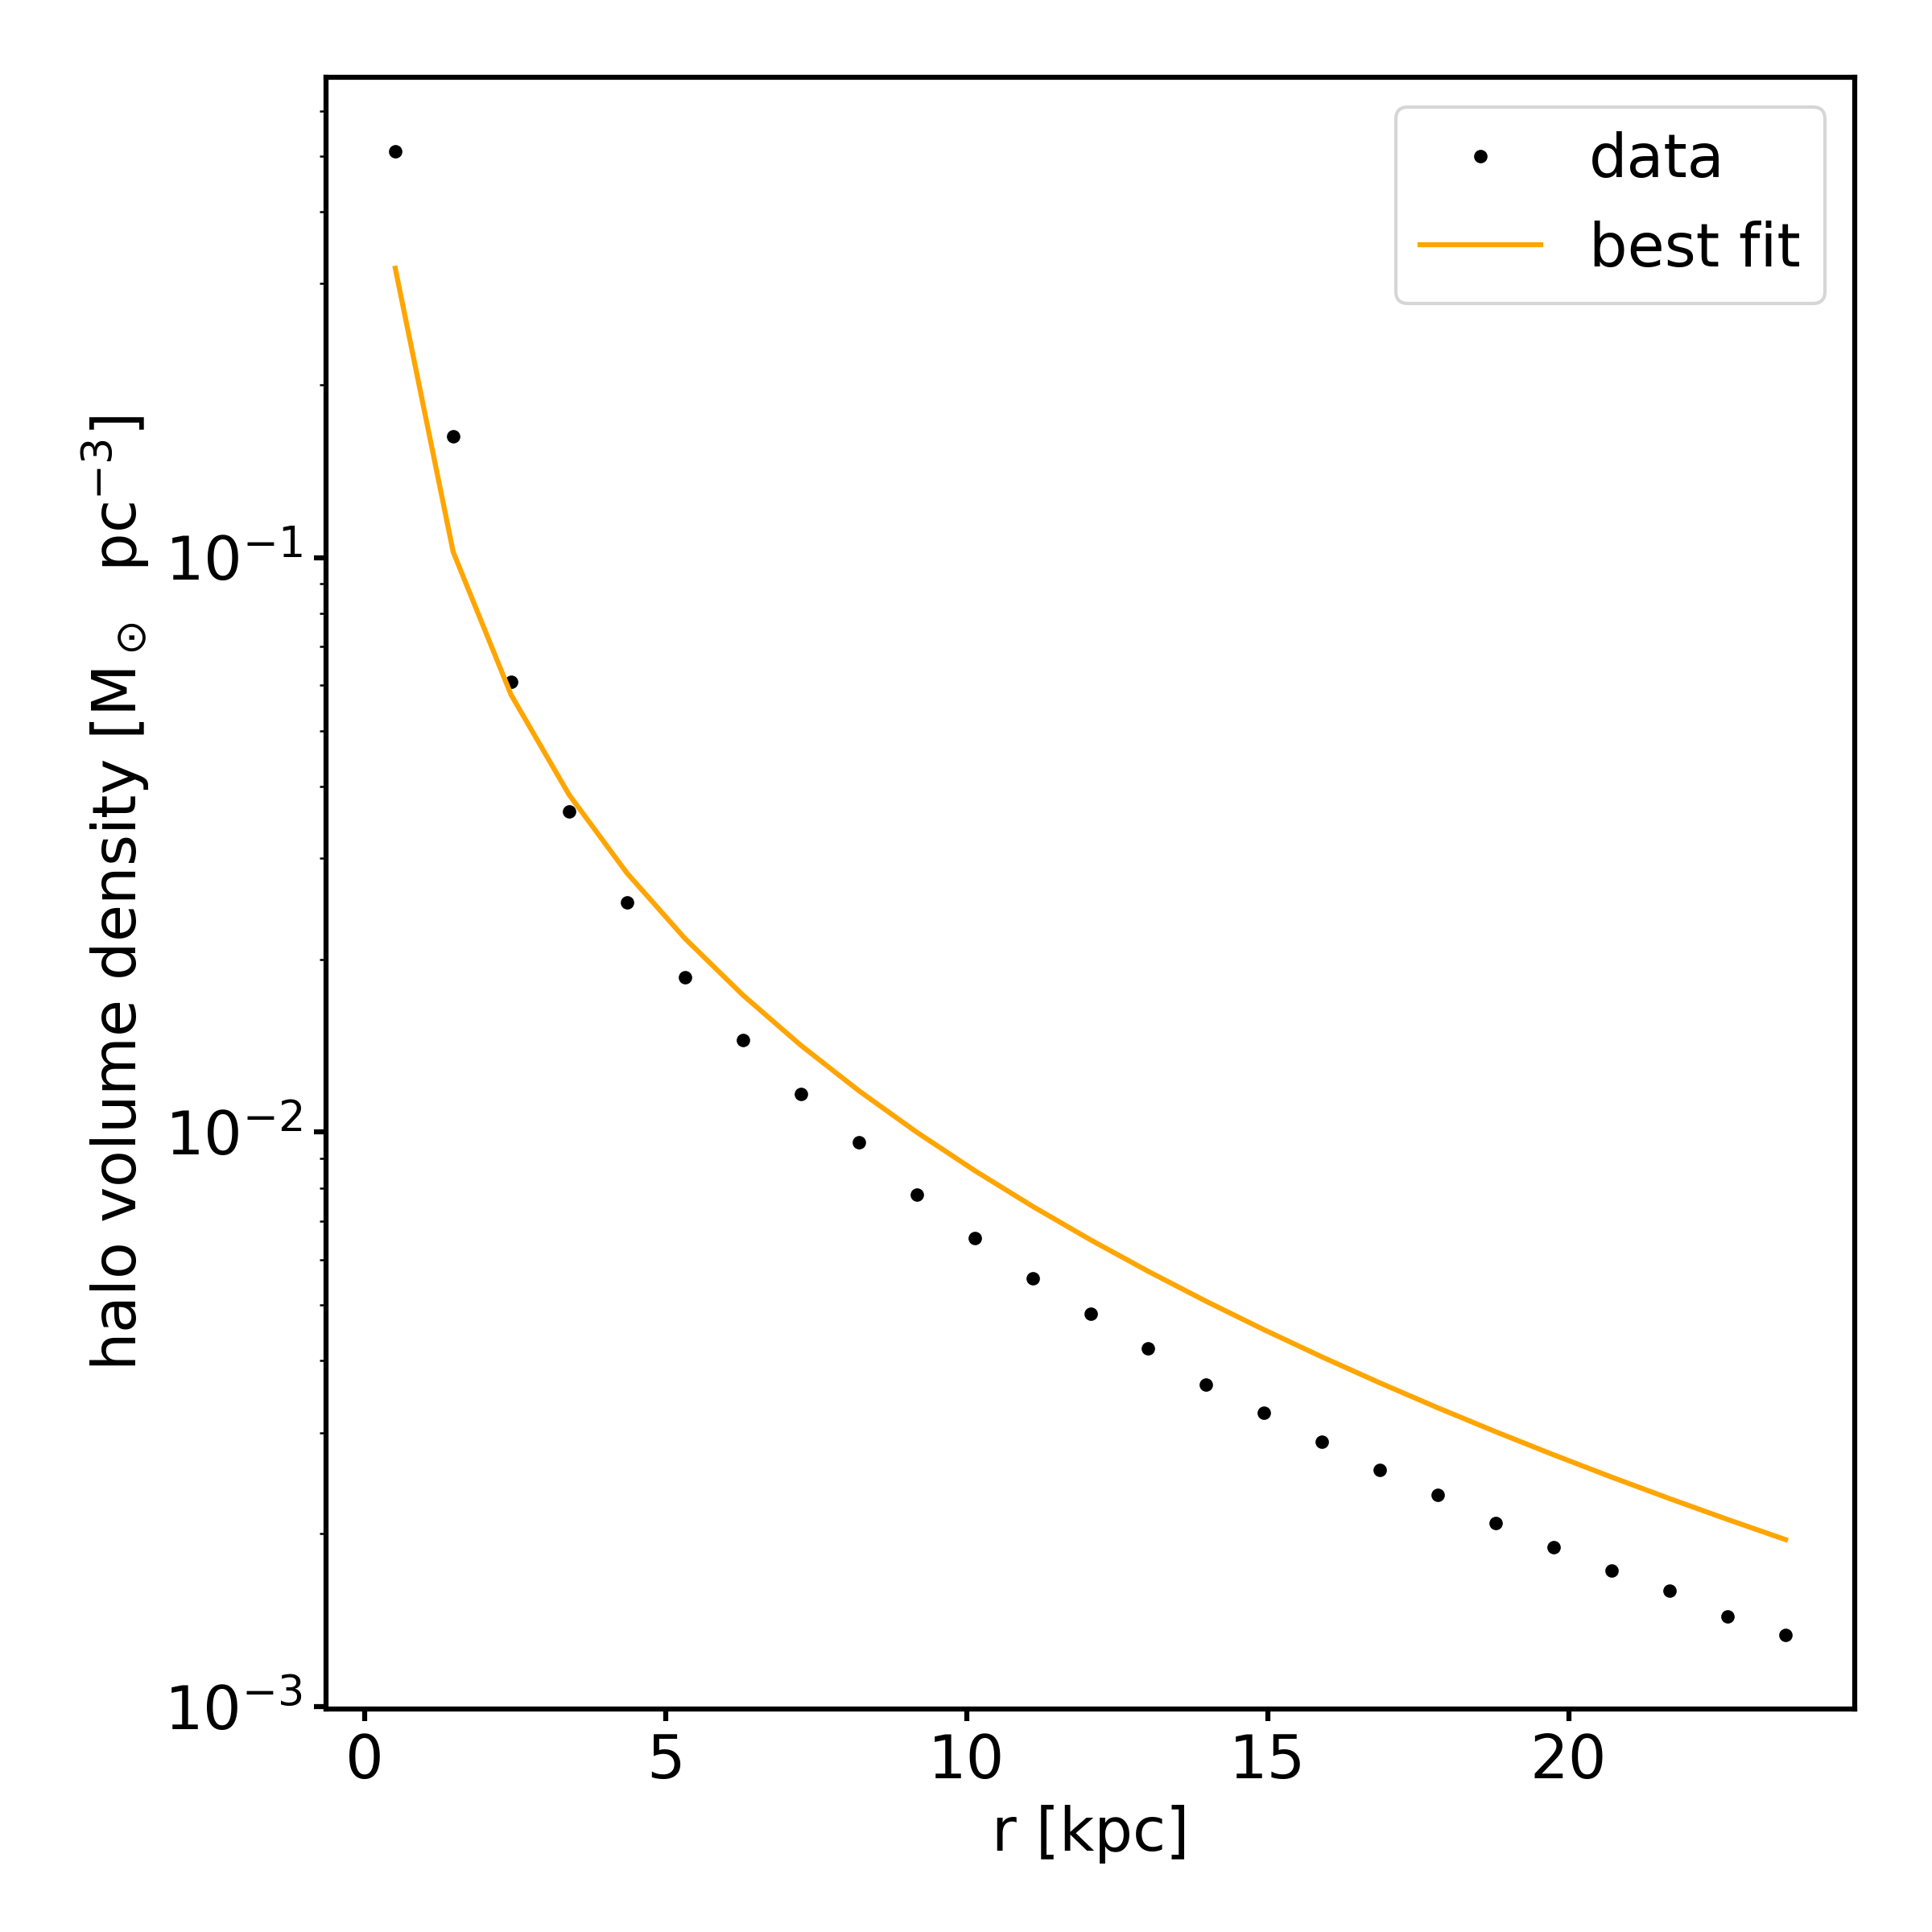
\includegraphics[width=\textwidth]{plots/Auriga/volume_dens_halo_fit_data.png}
	    \label{fig:halo_voldens_fit}
    \end{subfigure}
    \caption{Surface densities (upper row) and mass densities (lower row) of the components and their best fits at $\textit{z}=0$. Left (blue): stellar disk, middle (green): stellar spheroid, right (yellow): \ac{DM} halo.}\label{fig:single_pot_fits}
\end{figure}
\fi
\\
\begin{figure}[htbp]
\captionsetup{format=plain}
\centering
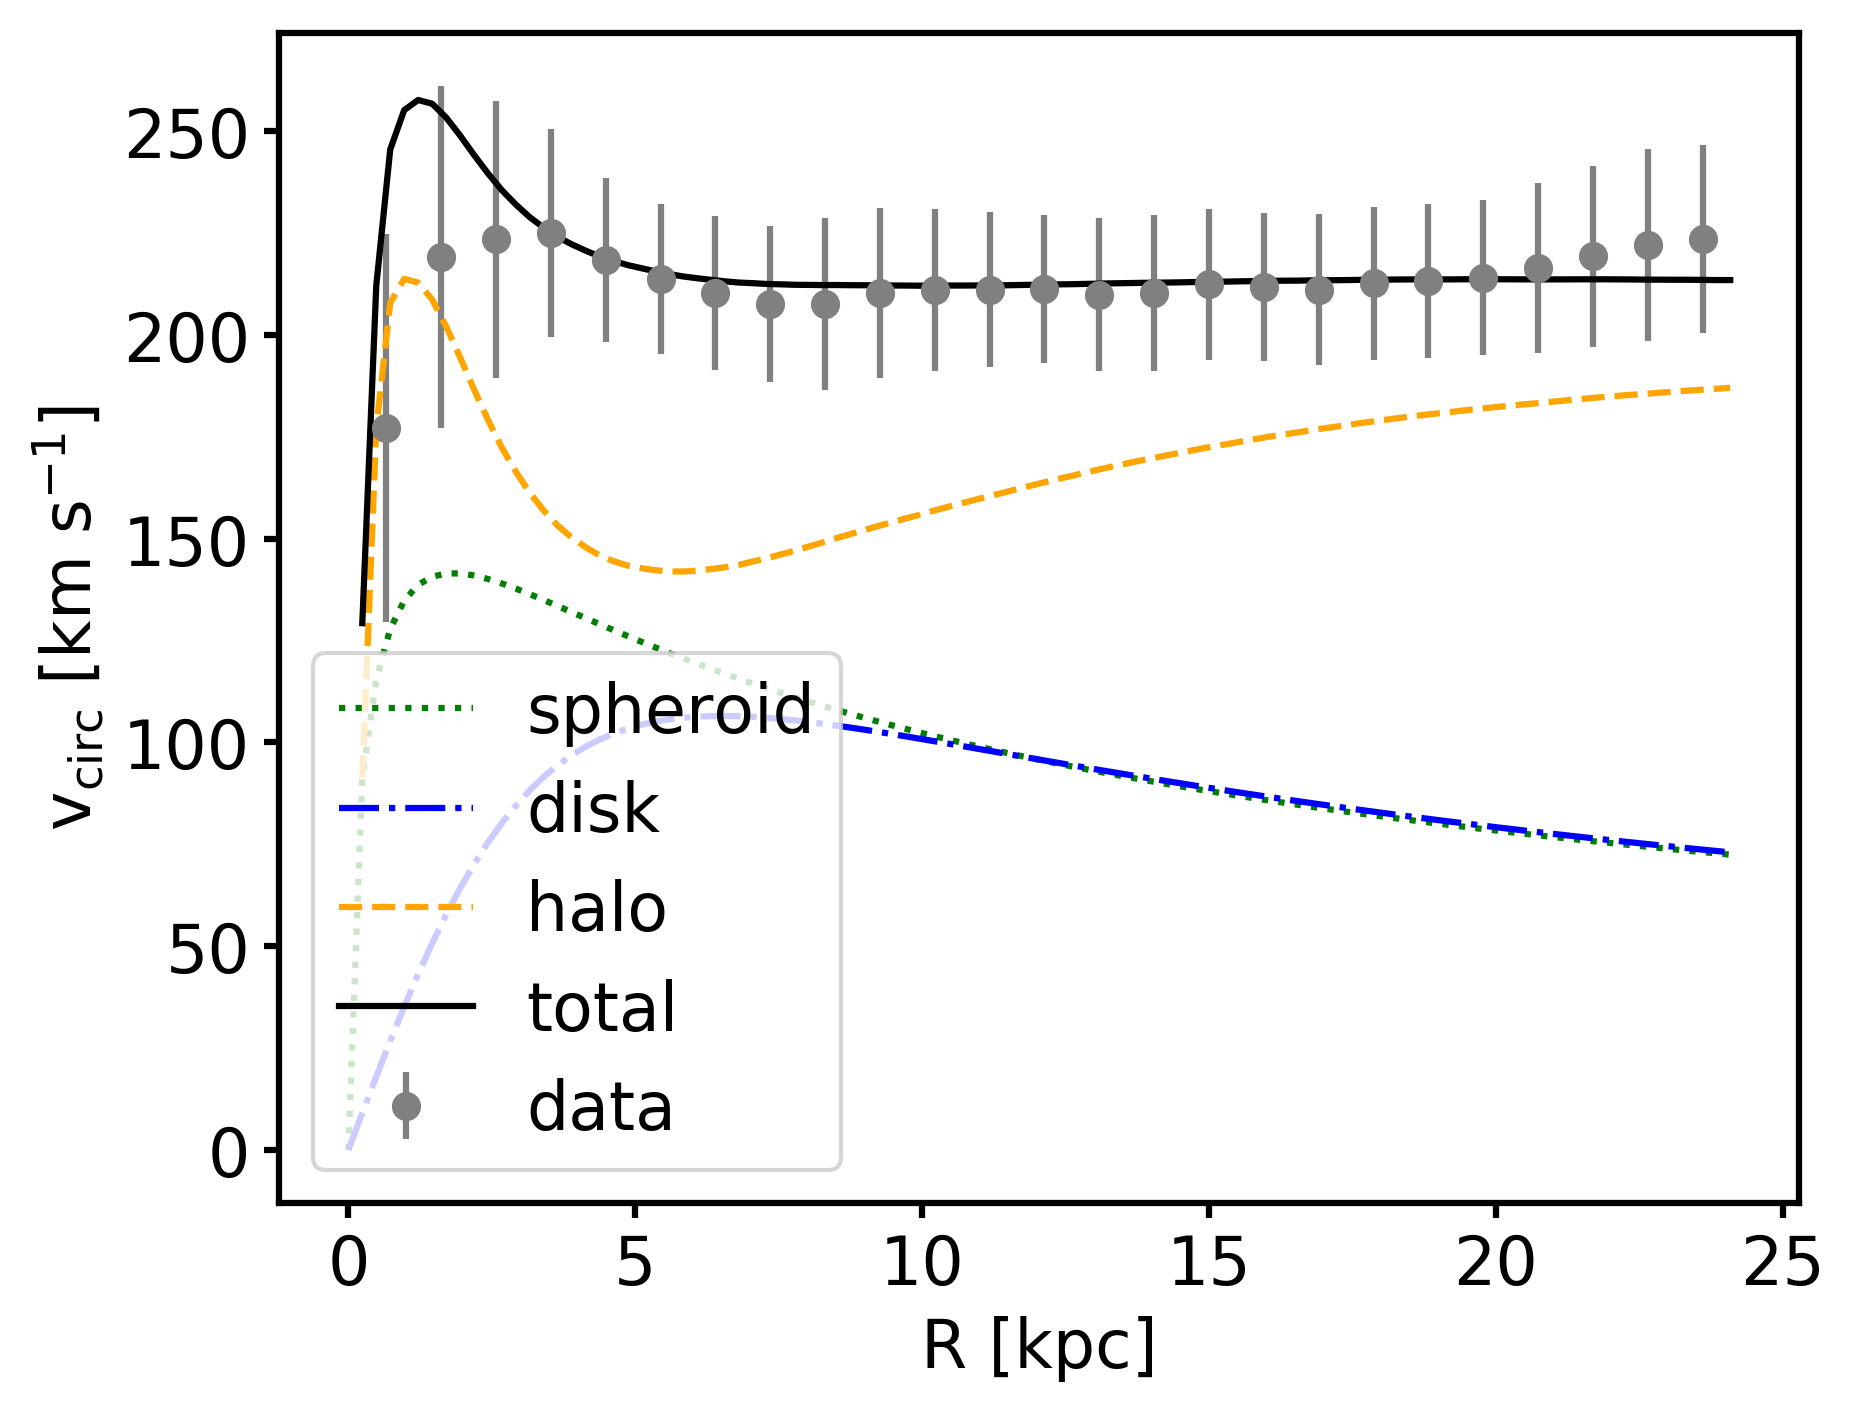
\includegraphics[width=0.8\textwidth]{plots/Auriga/best_fit_circular_velocity_via_formula_snap_127.png}
\caption{Circular velocity at \textit{z} = 0: data (grey circles), total (black solid line), disk (blue dashed dotted line), bulge (green dotted line) and halo (orange). The data is the mean tangential velocity of all stars which have $\epsilon > 0.95$. The other components and the total distribution are calculated analytically. The total curve matches the data within its errors. Disk and spheroid overlay in the outer parts which is due to the decomposition where their proportion is nearly $1:1$. The \ac{DM} distribution has a peak in the center. This is probably due to an underestimation of the spheroid component in the center which we can see find in the density fit in Figure \ref{fig:spheroid_fit}. In the outer parts ($R>R_0$), the curves behave as they are expected to do.}. \label{fig:circ_vel_fit}
\end{figure}
\\To verify the goodness of the total potential, we show the circular velocity curve in Figure \ref{fig:circ_vel_fit}. While in the innermost part the \ac{DM} proportion might be too high due to an underestimation of the stellar spheroid, the \ac{DM} proportion in the outer part seems correct. The disk is underestimated due to the sharp decomposition. In overall, the total circular velocity matches the data and the fit in the outer parts, where the particles we investigate in Section \ref{sec:Dynamics} are, is reliable.  

\subsubsection{Time evolution}
To make sure we can assume a slowly varying potential and to carry out investigations of e.g. the action evolution we need to know the potential for each snapshot. Using the fitting routine, we fit  a potential to each snapshot individually, without taking the results of the neighbouring snapshots into account, e.g. as a prior. Therefore, the fitting of the time evolution is unbiased in that sense. 
\begin{figure}%[htbp]
\captionsetup{format=plain}
\centering
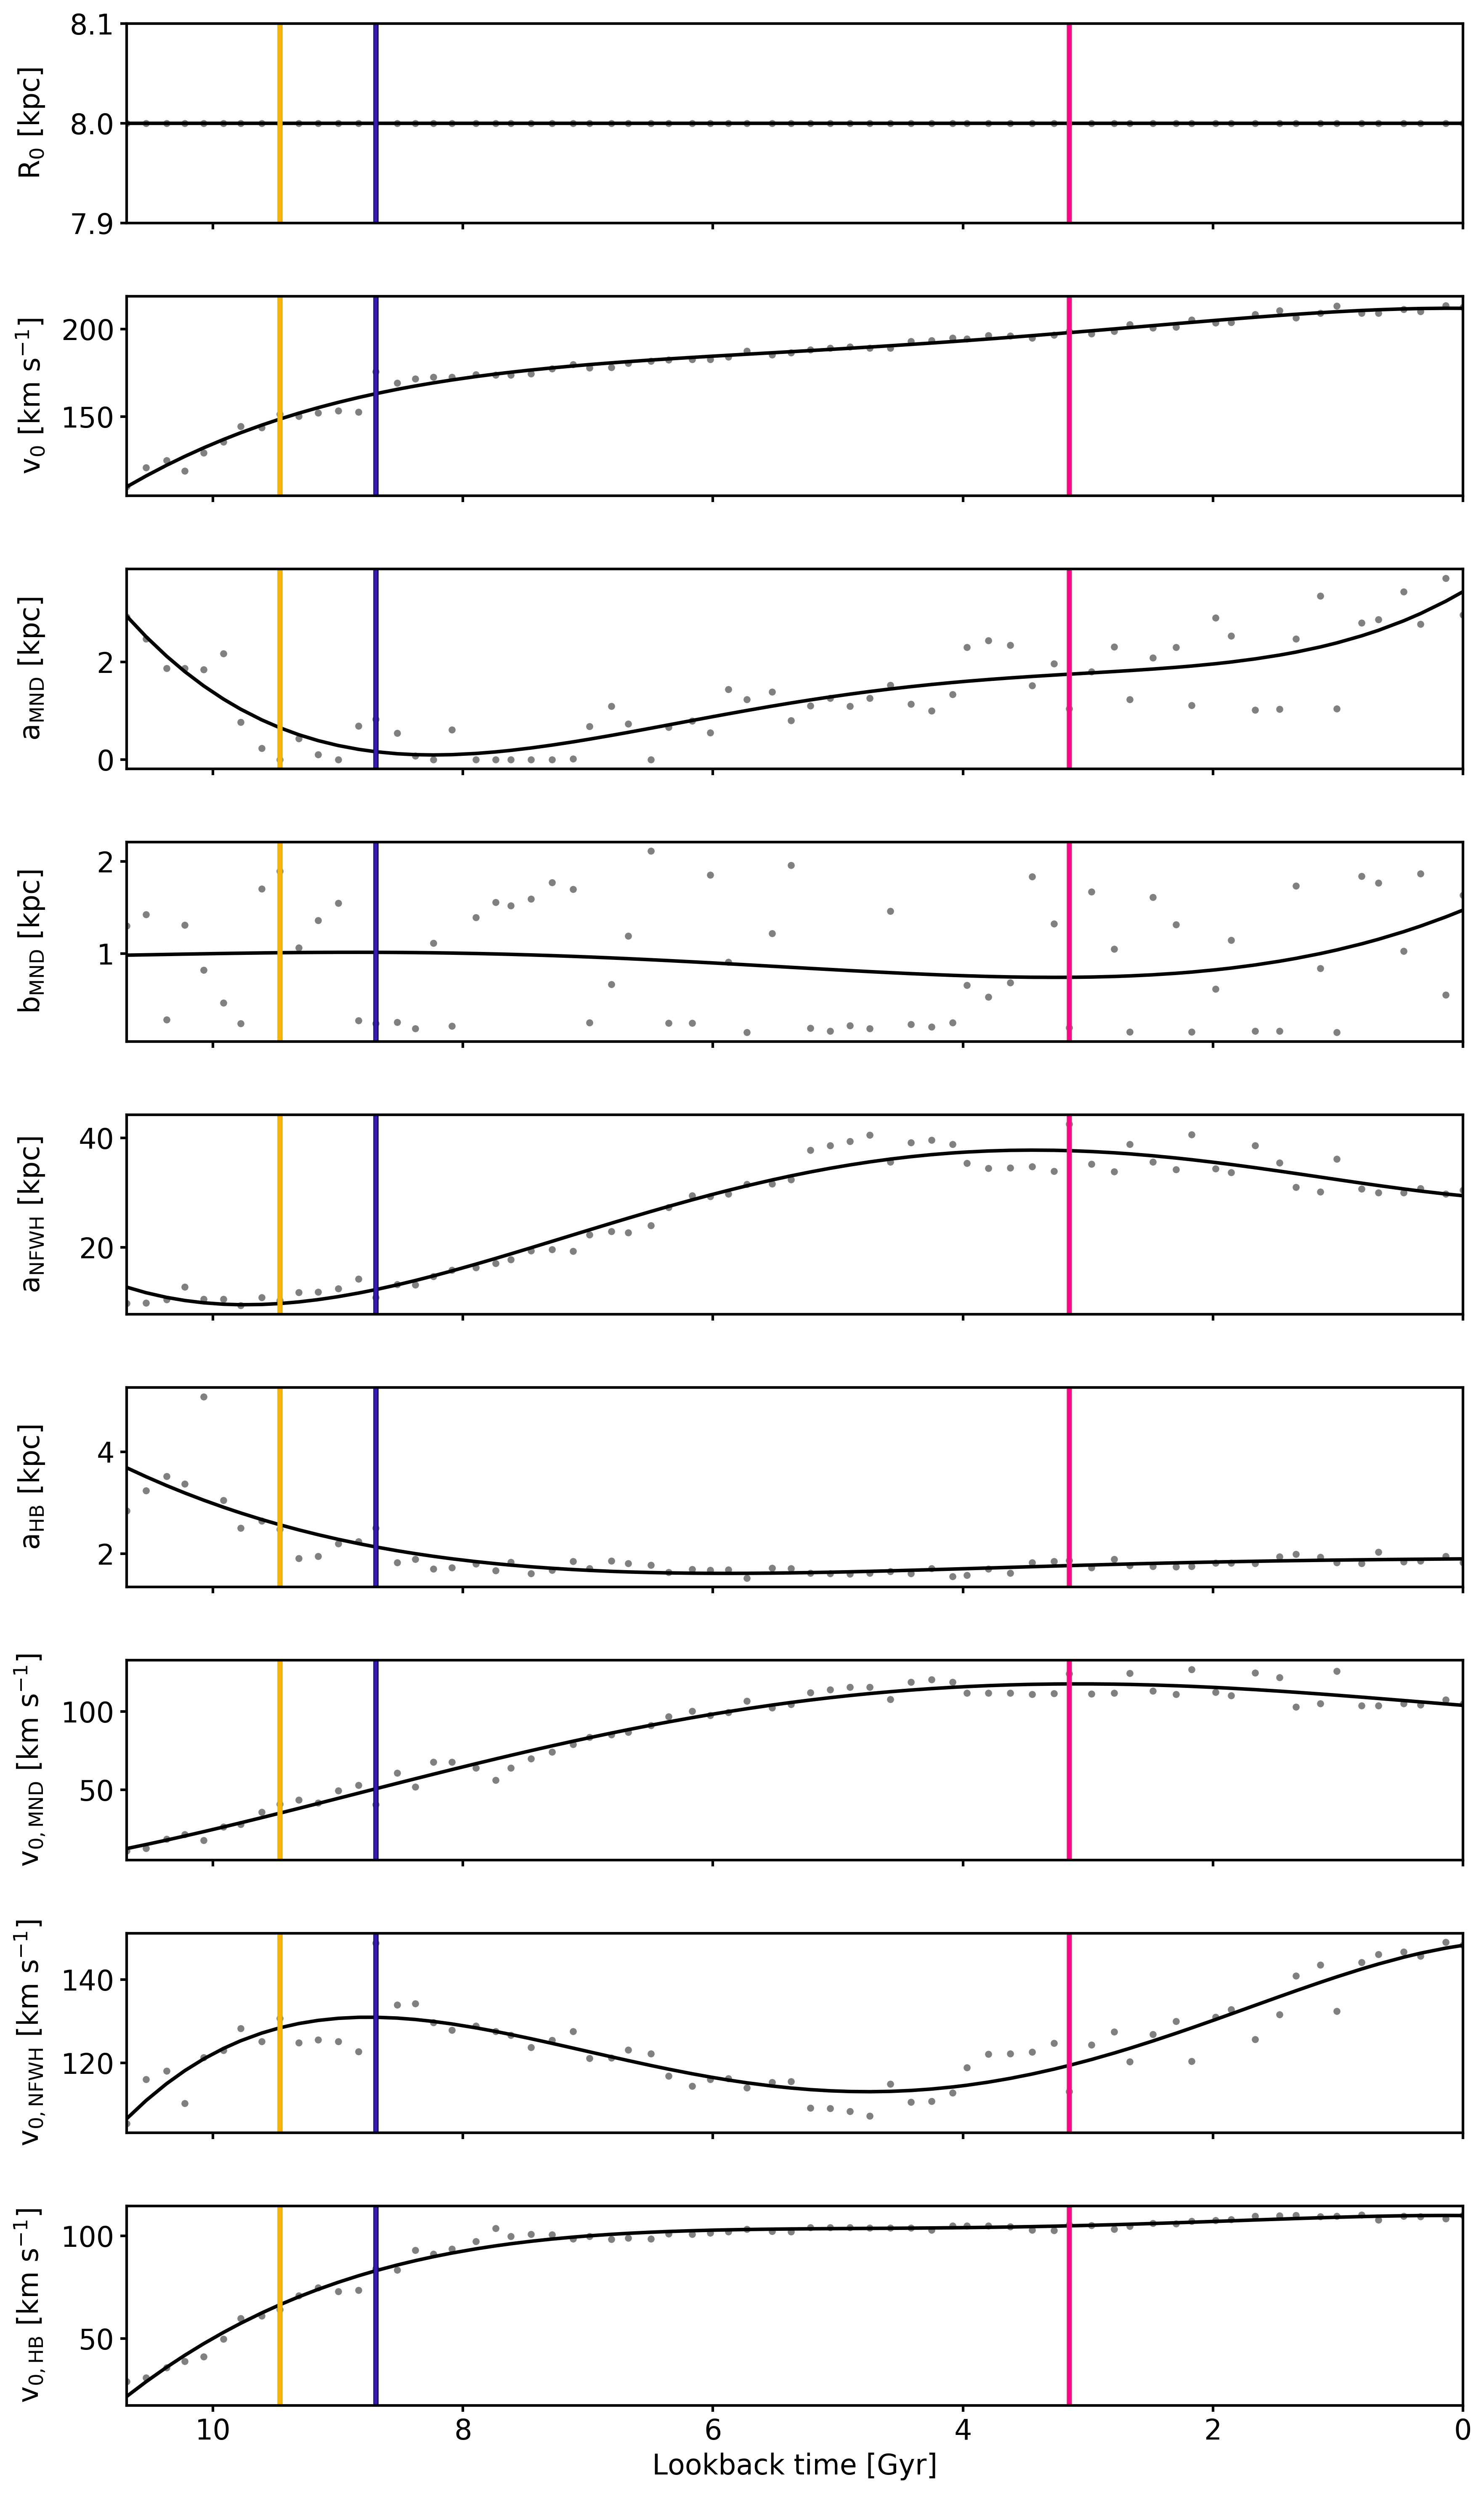
\includegraphics[width=0.7\textwidth]{plots/Auriga/fitted_potential_evolution_jan19.png}
\caption{Evolution of all fit parameters over time. $R_0$ and $v_0$ describe the overall evolution and the other parameters describe scale length - and height, if applicable - and their contribution to the circular velocity. The grey dots are the best fit values and the black lines are polynomial fits of 4th order for each parameter. The vertical lines mark the merger times of the three biggest merger events the main halo galaxy has experiences. The pink merger was the latest and biggest merger while the yellow merger contributed the least mass of these. In the first two panels, we see that the growth of the galaxy is continuous. The second merger flattened out the rise of the total circular velocity which is measured at $R_0 = \SI{8}{kpc}$. It is kept constant throughout the time evolution to see how within a constant radius the mass changes over time. The spheroid's parameters are very constant since the second merger, while the disk and the \ac{DM} halo are affected by the last merger. While the disk seems to grow in size, its contribution to the total circular velocity decreases. On the contrary, the \ac{DM} halo contracts but its contribution to the velocity rises more steeply. This shows, that these mergers have a strong impact on the evolution of the potential of this galaxy. Nevertheless, with the fits of the values we can still assume a slowly varying potential which is essential for the action evolution.}\label{fig:pot_val_evol}
\end{figure}
In Figure \ref{fig:pot_val_evol}, we show the time evolution of the potential parameters for the last \SI{10.5}{Gyr}. In the potential parameters, we see how the galaxy grows and how the growth is affected by mergers. The indicated mergers are described in more detail in the next Section and in Table \ref{tab:prog_overview}. The overall trend is very smooth and without any outliers. The spheroid remains very constant after the second biggest merger while the other components, especially the disk, have a larger scatter. The latest and biggest merger has a strong impact on the disk and the \ac{DM} halo. The fits of the values allow us to still carry out the action investigations (from Section \ref{subsec:GCs_action_space} on) under the assumption of a slowly varying potential (see also Section 3.6.1 in \citealp{Binney...Tremaine...2008}). 

\subsection{What not to do when fitting a gravitational potential to simulations}\label{subsec:wrong_pot_fit}
Even though the total circular velocity of our model matches the data the single component fits we carry out in Section \ref{subsec:best_fit_pot} have regions with large errors. We now explain some of the steps we took to develop this algorithm, what did not work and how we can deal with these errors.

\textbf{Fit the potential in one step}
In the first try, we worked with the three component analytic potential as well but we assumed that we can just fit the combined potential to the 'pot' value of a different amount of random particles (up to 1 million) of the simulation data. It resulted in a big overestimation of the halo and we had not control in giving each component its proportion.

\textbf{Decomposition}
To then fit a potential to each component we carried out a decomposition (Section \ref{subsubsec:decomp}). This decomposition only takes dynamically cold disk particles into account and does not set boundaries on the disk height. We therefore probably underestimated the disk while still having spheroid particles above and below the disk. Doing the decomposition kinematically is a good start but the recipe could expanded by some more complex disk characteristics. To get around the decomposition one could try to fit all stellar particles to a combination of disk and spheroid potential.

\textbf{Binning and weighting of the data}
Once we made a selection of disk and spheroid particles, we had to bin our densities to fit models to them. Depending on bin distances (e.g. linear or logarithmic), sizes and weights the focus of the fit is given to particular regions of the data. This has to be taken into account when preparing the data to be fitted.

\textbf{Fitting routines}
There are many methods of fitting models to data and these different methods offer a wide range of different implementations. We tried several for the different components. The first we used was scipy.optimize.minimize looking for the minimum of the relative error between data and model. This fitting routine find local minima. Therefore it sometimes ran into very unphysical parameters and found them to be the best fit. This routine was therefore to simple. We tried fitting the parameters with 'emcee' \textcolor{red}{reference} but this took very long and did not always converge so it was also not the best choice for us. Another scipy.optimize routine is 'differential\_evolution' which finds the global minima. So here again we minimized the relative error. This worked on the 1D models in the spherical potentials but did not in the 2D \ac{MN} potential as the algorithm just tried to set the model to 0 which would give in a small relative error but it resulted in extremely flat and elongated disks ($a_\mathrm{MND} = $ upper boundary and $b_\mathrm{MND} = 0$. The last fitting routine we then used on the \ac{MN} disk was scipy.optimize.curve\_fit which fits absolute differences between data and model but only requires the binned density and the model as input without the need to define how it minimizes the problem. This then worked for the disk the best. 

\textbf{Find proper fitting characteristics}
We fitted the stellar components to the stellar densities and the \ac{DM} profile to the potential value. We could also consider fitting all three components to their circular velocities which can also be calculated by the models. This would give us a constrain from the dynamical side and could make the fit better.

\\\\ Taking into account all these steps which we have to consider fitting a potential and getting still such a good circular velocity curve (Figure \ref{fig:circ_vel_fit} in the end, we are confident that this potential we got is good enough to carry out further investigations in this model but we also want to emphasize that this is a big component which can be improved.


%\textbf{Put in table with parameter comparison }